\documentclass[11pt]{article}
\usepackage{amsmath,amssymb,ctex}
\usepackage{tocloft}
\usepackage[a4paper, top=16mm, text={170mm, 248mm}, includehead, includefoot, hmarginratio=1:1, heightrounded]{geometry}
\def\pgfsysdriver{pgfsys-dvipdfm.def}
\usepackage{multido, pstricks,tikz} 
\usepackage[noautoscale]{youngtab} % for root/weight system and Young tableaux
\usepackage{amsthm}
\usepackage{hyperref}
	\hypersetup{
		pdftoolbar=true,  
		pdfmenubar=true,
		bookmarksnumbered=true,
	}

% \setCJKmainfont[
% 	ItalicFont = Adobe Kaiti Std ,
% 	BoldFont = SourceHanSerifSC-Bold ,
% 	]{Source Han Serif SC}

\theoremstyle{definition}
	\newtheorem{para}{}[section]
		\renewcommand{\thepara}{\thesection.\arabic{para}}
	\newtheorem{exa}[para]{Example}
\theoremstyle{plain}
	\newtheorem{lem}[para]{Lemma}
	\newtheorem{thm}[para]{Theorem}
	\newtheorem{pro}[para]{Proposition}
\renewcommand*{\proofname}{Proof}

\pagestyle{plain}

\title{Lie Algebra}
\author{buwailee}
% \date{}

\definecolor{shadecolor}{rgb}{0.92,0.92,0.92}

\newcommand{\no}[1]{{$(#1)$}}
% \renewcommand{\not}[1]{#1\!\!\!/}
\newcommand{\rr}{\mathbb{R}}
\newcommand{\zz}{\mathbb{Z}}
\newcommand{\aaa}{\mathfrak{a}}
\newcommand{\pp}{\mathfrak{p}}
\newcommand{\mm}{\mathfrak{m}}
\newcommand{\dd}{\mathrm{d}}
\newcommand{\oo}{\mathcal{O}}
\newcommand{\calf}{\mathcal{F}}
\newcommand{\calg}{\mathcal{G}}
\newcommand{\bbp}{\mathbb{P}}
\newcommand{\bba}{\mathbb{A}}
\newcommand{\osub}{\underset{\mathrm{open}}{\subset}}
\newcommand{\csub}{\underset{\mathrm{closed}}{\subset}}

\DeclareMathOperator{\im}{Im}
\DeclareMathOperator{\Hom}{Hom}
\DeclareMathOperator{\id}{id}
\DeclareMathOperator{\rank}{rank}
\DeclareMathOperator{\tr}{tr}
\DeclareMathOperator{\supp}{supp}
\DeclareMathOperator{\coker}{coker}
\DeclareMathOperator{\codim}{codim}
\DeclareMathOperator{\height}{height}
\DeclareMathOperator{\sign}{sign}

\DeclareMathOperator{\ann}{ann}
\DeclareMathOperator{\Ann}{Ann}
\DeclareMathOperator{\ev}{ev}
	\newcommand{\cc}{\mathbb{C}}
	\newcommand{\lag}{{\mathfrak{g}}}
	\DeclareMathOperator{\ad}{ad}
	\DeclareMathOperator{\Int}{int}
	\DeclareMathOperator{\sgn}{sgn}
	\DeclareMathOperator{\sym}{Sym}
	\DeclareMathOperator{\mult}{mult}
	\DeclareMathOperator{\lie}{Lie}

\begin{document}
	\maketitle
	\clearpage
	\tableofcontents
	\clearpage
	
	\section*{Outline}
\addcontentsline{toc}{section}{Outline}
\begin{itemize}

\item Lie群:具有微分流形结构的群。

因此左右平移是微分同胚,所以局部性质由单位元附近的那些元素决定。对于连通Lie群,则单位元附近的元素可以生成整个群的元素(即任意的群元都可以通过单位元附近的元素相乘组合得到)。

\item Lie群的Lie代数:Lie群单位元附近的局部线性化。

从前面的分析知道,Lie群的大部分性质由单位元附近的元素决定。由分析学的基本思想,在性质不算差的点,线性化后得到的切空间,将几乎完全能够(即两者之间存在微分同胚)反应那点附近的流形的结构。所以Lie代数能够确定Lie群的大部分性质。不过近似总归是近似,从Lie群到Lie代数,我们还是丢掉了不少东西,比如Lie群的拓扑结构。在半单Lie群的假设下,Lie代数和基本群能完全确定一个Lie群。

\item 为什么我们要研究Lie代数?

研究Lie代数的可行性来自于上述的Lie代数能够反应Lie群的许多性质。而研究Lie代数的动机很大程度在于Lie代数的代数结构比Lie群多,使得他比Lie群更方便研究。许多Lie群的性质(非代数的性质)在Lie代数中都表现为一些代数性质,这使得我们更方便操作。

\item 群表示:一个线性空间$V$,上面的可逆变换按复合构成一个群$\operatorname{GL}(V)$。而所谓的群表示,既是将已知的一个群$G$的元素看成某个空间$V$上的可逆的线性变换,并将群乘法变成线性变换的复合。换而言之,就是一个$G\to \operatorname{GL}(V)$群同态。

由于两个微分流形之间的光滑映射将诱导出切空间之间的映射,所以两个Lie群之间的光滑同态,将诱导出Lie代数的同态。而这就得到了Lie代数的表示的定义。

\item 为什么我们需要表示?

举个例子,狭义相对论的背景时空具有保持Minkowski内积的对称性,这个对称性对应的群是Poincar\'e群,如果不包含平移,则是Lorentz群$G$. 取$\Lambda \in G$,动量在$\Lambda$下进行如下变换
\[
	p^\mu \to \Lambda^\mu_{\phantom{\mu}\nu}p^\nu,
\]
在态矢量所处的空间来看,第一个惯性参考系来看的态矢量为$|p^\mu\rangle$,第二个惯性参考系来看的态矢量为$|\Lambda^\mu_{\phantom{\mu}\nu}p^\nu\rangle$,由于概率不依赖于参考系选取,两者之间应该靠某个线性幺正算符联系\footnote{这被称为Wigner定理:保持概率守恒的变换都将诱导出Hilbert空间上的一个幺正线性变换。},他依赖于$\Lambda$,记作$U(\Lambda)$,此时
\[
	U(\Lambda)|p^\mu\rangle = |\Lambda^\mu_{\phantom{\mu}\nu}p^\nu\rangle.
\]
现在再加上另一个$\bar\Lambda$,他应该将动量为$\Lambda^\mu_{\phantom{\mu}\nu}p^\nu$态的变成动量为$\bar{\Lambda}^\mu_{\phantom{\mu}\nu}\Lambda^\nu_{\phantom{\nu}\xi}p^\xi$的态,所以
\[
	U(\bar\Lambda)U(\Lambda)|p^\mu\rangle = U(\bar\Lambda)|\Lambda^\mu_{\phantom{\mu}\nu}p^\nu\rangle = \exp(i\theta(\Lambda,\bar\Lambda))|\bar{\Lambda}^\mu_{\phantom{\mu}\nu}\Lambda^\nu_{\phantom{\nu}\xi}p^\xi\rangle = \exp(i\theta(\Lambda,\bar\Lambda))U(\bar\Lambda \Lambda)|p^\mu\rangle,
\]
因此,
\[
	U(\bar\Lambda)U(\Lambda)= \exp(i\theta(\Lambda,\bar\Lambda)) U(\bar\Lambda \Lambda).
\]
有个相位是因为,相位不影响态。尽管这个相位在物理上是等价的,在数学上我们不能直接无视其存在。还好,如果群的性质不太差,或者我们选个性质更好的群来代替他,则关于任意的两个变换,这个相位我们可以全部搞成1。所以我们可以得到
\[
	U(\bar\Lambda)U(\Lambda) = U(\bar\Lambda \Lambda),
\]
此时$U$就是一个表示。因此,背景时空对称性能够诱导出态矢量上的对称性,利用的手段就是群表示。

那么,有了这个群表示,我们就有Lie代数的表示,Poincar\'e群的Lie代数,现在就变成了一些态矢量所处的Hilbert空间上的算符,而这些就是动力学算符。这就是说:对称性诱导出了动力学算符,而动力学量的不可约表示完成了单粒子分类。

\item 从Lie代数到Lie群:Ado定理,所有实Lie代数都同构于$\mathfrak{gl}(n,\rr)$的子代数。所以每一个实Lie代数都可以实现为某个Lie群的Lie代数的子代数。同时,对于任意的连通Lie群,他一定存在一个万有覆叠空间(单连通的覆叠空间),他有着Lie群结构,且和原来的Lie群有着相同的Lie代数。

从这里可以看到,Lie代数并不在意Lie群很细致的拓扑结构,这就是他丢失的东西。拓扑结构(作为整体结构)有时候很重要,比如对于无质量粒子,他的自旋(或者此时应该叫helicity)只能取整数或者半整数就来自于表征对称性的群的拓扑结构。

\item 从Lie代数同态到Lie群同态:如果$h$是$\lag_1\to \lag_2$之间的Lie代数同态,且$\lag_1$是一个单连通Lie群$G_1$的Lie代数,$\lag_2$是一个连通Lie群$G_2$的Lie代数,则存在唯一的Lie群同态$\bar{h}:G_1\to G_2$,使得$\bar{h}$诱导的Lie代数同态即$h$.

将其应用到表示,则有Lie代数的表示唯一确定单连通Lie群的表示。

\item 为什么要复表示?

其一,物理上的态所处的Hilbert空间是在复数域上面的,所以我们需要复表示。其二,比如最简单的$U(1)$群,他的非平凡表示,对于实数域上来说,是$2$维的,即$\mathrm{SO}(2)$,而在复数域上是一维的,即他本身。其三,复数域是代数闭的。

\item 为什么要研究半单复Lie代数?

半单性是紧性在代数上的合理推广。对于半单复Lie代数$\lag$,我们可以找到一个紧Lie群的Lie代数$\mathfrak{k}$(这样的Lie代数称为紧Lie代数),使得$\lag\cong \mathfrak{k}\otimes \cc$. 反过来,任意的紧Lie群的Lie代数$\mathfrak{k}$,他的复化$\mathfrak{k}_{\cc}:=\mathfrak{k}\otimes \cc$是一个半单复Lie代数。所以我们一旦完全分类了半单复Lie代数,也就完全分类了紧Lie代数。

前面说了,半单性是紧性在代数上的合理推广。这点的表现比如,对于半单复Lie代数来说,他的任意有限维表示都是完全分解的,即可以分解为不可约表示的直和。代数上,这被称为Weyl定理,整个半单复Lie代数以及半单实Lie代数的分类就是由Weyl完成的。

\item 如何分类半单复Lie代数呢?

靠表示论,Lie代数在自己身上有一个自然的表示,被称为伴随表示。Lie代数极大交换子代数的元素在伴随表示的时候作为线性算符的本征值将完全决定Lie代数的结构。

\item 如何分类半单复Lie代数的有限维复表示?

首先依靠于完全分解性,我们可以只关注不可约表示。对于不可约表示,我们只需要给出那些可以同时测量的量子数,即极大交换子代数中元素的所有本征值,这样的本征值我们称作权,所以我们只需要确定所有的权就可以了。在权之中,我们可以挑出一个最大的权,他确定了其他所有的权。举个例子,对于自旋的表示,他的极大交换子代数由$J^3$生成,对应一个量子数$j$,他的权为$\{-j,-j+1,\dots,j-1,j\}$,而最大权就是$j$.

\end{itemize}

	\section{一些基本的定义}

% \subsection*{群的定义}

% \para 一个集合$G$,上面有一个运算$*$满足结合率$a*(b*c)=(a*b)*c$,且存在唯一一个元素$e$使得$a*e=e*a=a$对任意的$a\in G$都成立,同时,任取$g\in G$都存在一个元素$h\in G$使得$g*h=h*g=e$,这个元素称为$g$的逆,通常写作$g^{-1}$. 下面写群运算的时候直接无视掉他的符号,即$g*h$写作$gh$. 

% 如果群$G$的一个子集$H$,按照继承于大的群上的运算,满足群的那些公理,则称$H$为群$G$的一个子群。显然,两个子群的交依然是一个子群。

% 简单来说,群就是一个集合,上面有一种存在单位元的满足结合律的运算,而且对每一个元素存在逆元。

% \para 考虑一个集合到自身的所有双射(一般我们称为变换),这自然构成一个群。反过来,群的每一个元素都可以通过左乘看作群到群的一个双射,自然这就是一个变换。因此,群也可以理解成变换构成的集合。

% 有人说,群就是对称,这不是很正确的说法。所谓对称,就是说某些变换下不变的某种性质。所以将对称与群联系起来的正确说法是:如果某种结构在群$G$的变换下不变,那么我们就称呼这是一个具有$G$对称性的结构。

\subsection*{Lie群和Lie代数的定义}

\para[Lie群] 若一个群$G$同时具有相容的群结构和微分流形结构,则群$G$是一个Lie群。所谓相容的,就是说,群运算是可微的,所谓的微分流形,就是广义的曲面。
\endpara

下面我们给出一些Lie群的例子,它们都属于矩阵群,即群元都是矩阵,且矩阵元的取值都是连续的。此时,对一个依赖于实参数$t$的矩阵$A(t)$来说,上面的求导定义为
\[
	\frac{\dd A(t)}{\dd t}=\lim_{t\to 0}\frac{A(t)-A(0)}{t}.
\]
求导运算很容易验证满足
\[
	\frac{\dd A(t)B(t)}{\dd t}=A'(t)B(t)+A(t)B'(t),
\]
或者更一般的,对于一个双线性型$K(*,*)$,成立
\[
	\frac{\dd }{\dd t}K(A(t),B(t))=K(A'(t),B(t))+K(A(t),B'(t)).
\]
这些都可以从求导的定义来直接检验。

\para[一般线性群和特殊线性群] 作为第一个例子,我们考虑一个矢量空间$V$,所有可逆线性变换(或者说矩阵)$A:V\to V$按照复合(或者说矩阵乘法)构成了一个群,他被记作$\operatorname{GL}(V)$,被称为一般线性群。当$V=\rr^n$的时候,一般线性群记作$\operatorname{GL}(n)$,当$V=\cc^n$的时候,一般线性群记作$\operatorname{GL}(n,\cc)$.

在$\operatorname{GL}(V)$中,那些行列式为$1$的矩阵构成了一个子群$\operatorname{SL}(V)$,因为行列式为1的矩阵的逆以及乘积的行列式都还是1. 从线性代数的几何直观,行列式为1的矩阵保持体积。
\endpara

\para[正交群和幺正群]  现在设$\rr^n$上面具有一个内积$(v,w)=\sum_{i=1}^n v_i w_i$,$\cc^n$上有一个内积$\langle v,w\rangle=\sum_{i=1}^n v^*_i w_i$,其中$v_i^*$是$v_i$的复共轭。从几何上面来看,内积给出了一个矢量的长度,以及两个实矢量之间的夹角。

考虑一个实矩阵$A:\rr^n \to \rr^n$,他将矢量$v$和$w$变成了$Av$和$Aw$,如果对任意的$v$和$w$都使得$(Av,Aw)=(v,w)$成立,则称$A$是一个正交矩阵。正交矩阵在这里表征的是保持内积的对称性,几何上来看,矢量的长度和两个矢量的夹角不变。下面要验证所有的正交矩阵构成一个群,这个群被记作$\mathrm{O}(n)$,称为正交群。

由于
\[(v,w)=(Av,Aw)=(A^TAv,w),\]
且内积非退化,所以$A^TA=I$,所以$\det (A^TA)=\det(A)^2=1$,于是$\det(A)\neq 0$,这也就推出$A$是可逆的,所以我们可以把正交矩阵的定义改成:$A^T=A^{-1}$.

随后,我们检验正交矩阵$A$和$B$的复合(或者说乘积)也是正交矩阵,$(AB)^T=B^TA^T=B^{-1}A^{-1}=(AB)^{-1}$,同时,由于$(A^{-1})^T=(A^T)^{-1}=(A^{-1})^{-1}=A$,因此$A$的逆也是一个正交矩阵。所以正交矩阵们按照矩阵乘法(或者说线性映射复合)成群。

类似地,考虑一个复矩阵$A:\cc^n \to \cc^n$,如果对任意的$v$和$w$都使得$\langle Av,Aw\rangle =\langle v,w\rangle $成立,则称$A$是一个幺正矩阵。由于$\langle Av,Aw\rangle=\langle A^{\dag}Av,w\rangle$,所以幺正矩阵也可以定义为满足$A^\dag A=I$的矩阵。同上可以类似验证所有的幺正矩阵构成一个群,这个群被记作$\mathrm{U}(n)$,称为幺正群。
\endpara

\para 已经看到$\operatorname{SL}(n)$,$\mathrm{O}(n)$是$\operatorname{GL}(n)$的子群,$\operatorname{SL}(n,\cc)$和$\mathrm{U}(n)$是$\operatorname{GL}(n,\cc)$的子群,那么
\[
	\mathrm{SO}(n)=\operatorname{SL}(n)\cap \mathrm{O}(n),\quad \mathrm{SU}(n)=\operatorname{SL}(n,\cc)\cap \mathrm{U}(n),
\]
也分别是$\operatorname{GL}(n)$和$\operatorname{GL}(n,\cc)$的子群。

\para[Lie群$\operatorname{SL}(2,\cc)$] 现在来看$\operatorname{SL}(2,\cc)$. 任何一个复可逆$2\times 2$矩阵都可以唯一分解(极分解)为$
\lambda=u\exp(h)$,其中$u$幺正而$h$是Hermite矩阵。现在假如$\det \lambda=1$,则
\[
\det(u)\exp(\tr(h))=1
\]
于是$\det(u)=1$而$\tr(h)=0$. $u$的一般形式为
\[
u=
\begin{pmatrix}
a+ib&c+id\\
-c+id&a-ib
\end{pmatrix},
\]
且满足$a^2+b^2+c^2+d^2=1$,因此其拓扑上等价为3-球面$\mathbb{S}^3$. 而$h$的一般形式为
\[
h=\begin{pmatrix}
e&f-ig\\
f+ig&-e
\end{pmatrix},
\]
拓扑上等价于$\rr^4$,因此$\operatorname{SL}(2,\cc)$在拓扑上等价于$\rr^4\times \mathbb{S}^3$. 
\endpara

\para[Lie代数] 所谓的Lie代数,就是Lie群在单位元处的切空间,是Lie群的局部近似。由于每一个群元左作用都是微分同胚,比如对于$g\in G$,$l_g:h\mapsto gh$是一个同胚,他的逆就是$l_{g^{-1}}$,这样一个映射,将$e$映射成$g$,并且同时,将$e$处的切矢量$v$,映射到了$g$出的一个切矢量$(l_g)_{*g}v$. 改变$g$,这样我们就得到了$G$上的一个矢量场,这样的矢量场被称为一个左不变矢量场$V$. 显然,一个Lie代数的元素对应一个左不变矢量场。
\endpara

\para[指数映射]
有了矢量场,我们就可以谈论其的积分曲线,换而言之,找一条曲线,使得他在每一点的切矢量刚好和矢量场在那点的矢量一样。积分曲线可以局部唯一存在,这是常微分方程告诉我们的结论。对于Lie群的左不变矢量场而言,由于每一点的切矢量都是同胚$l_g$复制过去的,所以每一点附近的积分曲线求解都差不多,这就意味着,先在一点附近求解出一条积分曲线,然后在这条积分曲线的接近末端,我们可以再求解一条新的积分曲线,他和原本那条部分重合,合起来就得到了一条更长的积分曲线,然后再慢慢一直延拓下去。

考虑$v$是一个Lie代数的元素,$V$是他的左不变矢量场,记$\exp(t,v)$是$V$的一条在$t=0$时刻经过$e$的一条$V$的积分曲线,由于上段的陈述,我们知道$t$可以从$-\infty$取到$\infty$. 我们可以发现$\exp(t,v)=\exp(1,tv)$,这是因为左不变矢量场每一点的切矢量都是同胚$l_g$复制过去的,所以如果初速度是$v$的$t$倍,那么处处速度是原本速度的$t$倍,因此,原本需要跑$t$时间的路,现在只需要$1$时间了。正规的证明只要用微分方程解的唯一性即可。因此,对于$\exp(t,v)$而言,我们可以将其写作$\exp(tv)$而并不丧失什么信息。

一个不那么显然的等式是$\exp(tv)\exp(sv)=\exp((t+s)v)$,注意到这和复数$\exp$函数的相似性,这也就是为什么我们称呼他为指数映射的原因。这个等式的证明只要考察$\exp(sv)$处开始的一条$V$的积分曲线,然后利用积分曲线的唯一性即可。

% 利用上面的等式以及$\exp(0v)=e$,我们得到$\exp(v)^{-1}=\exp(-v)$.
\endpara

对于矩阵群而言,
\[
	\exp(tA)=I+\sum_{n=1}^\infty \frac{(tA)^n}{n!}=\sum_{n=0}^\infty \frac{(tA)^n}{n!},
\]
更严格的证明可以参见附录,这里提供一种思路。我们考虑$\exp(tA)$,将其在$t=0$附近展开,有$\exp(tA)=I+tA+O(t^2)$,然后对于任意的正整数$n$和固定的$t$我们有
\[
	\exp(tA)=\left(\exp(tA/n)\right)^n=\left(I+\frac{t}{n}A+O\left(\frac{1}{n^2}\right)\right)^n,
\]
然后令$n\to\infty$,就有$\exp(tA)=\lim_{n\to\infty}\left(I+\frac{t}{n}A\right)^n$. 使用二项式展开,就可以得到其级数展开
\[
	\exp(tA)=1+\sum_{n=1}^\infty \frac{(tA)^n}{n!}=\sum_{n=0}^\infty \frac{(tA)^n}{n!},
\]
最后$t=1$即可。

\begin{pro}
矩阵的指数映射联系了行列式和迹,具体来说就是
\[
	\det(\exp(A))=\exp(\tr(A)).
\]
\end{pro}

\begin{proof}
证明见附录。
\end{proof}

\para 上面描述了从Lie代数到Lie群的手段,即利用积分曲线。每一个Lie代数都可以往上得到Lie群里面的元素。反过来,要得到Lie代数的元素只要求导即可。
\endpara 

$\operatorname{GL}(n,\cc)$的Lie代数$\mathfrak{gl}(n,\cc)$就是$\mathrm{M}(\cc^n)$,即$\cc^n\to \cc^n$的所有矩阵全体,因为任取$A\in \mathrm{M}(\cc^n)$,我们都有$\det(\exp(tA))=\exp(t \tr(A))\neq 0$,故$\exp(tA)\in \mathrm{M}(\cc^n)$.

$\operatorname{SL}(n,\cc)$的Lie代数$\mathfrak{sl}(n,\cc)$就是那些满足$\tr(A)$的矩阵,或者说,迹零矩阵构成的矢量空间。$\operatorname{SU}(n)$的Lie代数$\mathfrak{su}(n)$中的元素首先是迹零矩阵,然后也满足
\[
	0=\left.\frac{\dd}{\dd t}\right|_{t=0}\exp(tA)\exp(tA^{\dag})=A^\dag+A,
\]
或者引入一个$i$,将其写作$(iA)^\dag=iA$,所以$\operatorname{SU}(n)$的Lie代数$\mathfrak{su}(n)$就是那些满足$A=A^\dag$的迹零矩阵$A$构成的矢量空间。

对于$\mathrm{O}(n)$的Lie代数$\mathfrak{o}(n)$,利用
\[
	0=\left.\frac{\dd}{\dd t}\right|_{t=0}\exp(tA)\exp(tA^{T})=A^T+A,
\]
所以$\mathfrak{o}(n)$就是那些反对称的矩阵构成的矢量空间。由于反对称矩阵自然是迹零的,所以$\mathrm{SO}(n)$的Lie代数$\mathfrak{so}(n)$也是$\mathfrak{o}(n)$.

\para[Lie括号] 通过将矢量场看成Lie群上光滑函数的导数,我们可以定义Lie代数上的如下算符$[X,Y]=XY-YX$,对于矩阵群的Lie代数来说
\[
	[A,B]=AB-BA,
\]
其中$A$和$B$之间为矩阵乘法。证明可以参见附录。
\endpara

通过直接的计算,Lie代数上满足:
\begin{enumerate}
	\item[(1)] $[X,Y]=-[Y,X]$,
	\item[(2)] $[X,[Y,Z]]+[Y,[Z,X]]+[Z,[X,Y]]=0$.
\end{enumerate}
第一条反对称性从矢量场的$[X,Y]=XY-YX$来看是显然的。而第二条称为Jacobi恒等式,直接计算即可验证。可以如下记忆Jacobi恒等式,$X$, $Y$和$Z$的三种右手方向构成的置换和为$0$,或者说,$[X_i,[X_j,X_k]]$中$ijk$是$123$的偶置换。

\subsection*{表示的定义}

\para[表示] Lie群$G$的有限维表示是一个二元组$(\rho,V)$,其中$V$是一个有限维矢量空间\footnote{我们以后会一直默认有限维,所以就在以后略去有限维,除非特别声明。},前者$\rho:G\to \operatorname{GL}(V)$是一个群同态,即满足$\rho(gh)=\rho(g)\rho(h)$.

设Lie群$G$的Lie代数是$\lag$,那么他的表示是一个二元组$(\pi,V)$,前者$\pi:\lag \to \mathfrak{gl}(V)=\mathrm{M}(V)$,满足
\[
	\pi([A,B])=[\pi(A),\pi(B)].
\]
\endpara

粗略来说,表示就是将$G$或者$\lag$里面的元素看成$V$上的线性变换。Lie代数的表示的定义和Lie群的表示的定义是相容的,一旦有一个Lie群的表示,将其求导也就得到了其Lie代数的表示。为了避免微积分,所以我们这里就直接给出Lie代数表示的定义了。

\para[不可约表示] 如果对于群$G$一个表示$(\rho,V)$,存在$V$的一个子空间$W$使得$\rho(G)W\subset W$,则$(\rho,W)$也构成一个表示,他被称为$(\rho,V)$的一个子表示。每一个表示都存在两个平凡的子表示,一个是本身,一个是零表示,即$(\rho,\{0\})$. 除去这两个子表示,如果该表示没有其他子表示,则称这个表示为一个不可约表示。类似地,我们可以定义出什么叫Lie代数$\lag$的不可约表示。

\para 对于一个对象的两个表示$(\rho,V)$和$(\pi,W)$,我们可以定义直和表示,通过
\[
	(\rho(g),\pi(g))(v,w)=(\rho(g)v,\pi(g)w).
\]
如果一个表示可以分解成一些不可约表示的直和,则称该表示是完全可约的。

\para[伴随表示] 对于矩阵群$G$,他的Lie代数是$\lag$,考虑如下表示$(\mathrm{Ad},\lag)$
\[
	\mathrm{Ad}(U)B=UBU^{-1},
\]
他被称为伴随表示,对于一般的Lie群的伴随表示的定义,参见附录。
\endpara

我们令$U=\exp(tA)$,并将其在$t=0$处求导,得到
\[
	\left.\frac{\dd}{\dd t}\right|_{t=0}\mathrm{Ad}(\exp(tA))B=AB-BA=[A,B],
\]
我们将其记作$\ad(A)B:=[A,B]$,这是一个Lie代数的表示,满足
\[
	\ad([A,B])=[\ad(A),\ad(B)],
\]
以及成立
\[
	\ad(A)([B,C])=[\ad(A)B,C]+[B,\ad(A)C],
\]
这些证明都是直接的。最后两个式子和Jacobi恒等式等价。

\para 由于$\ad$是$\mathrm{Ad}$的导数,所以$\mathrm{Ad}(\exp(tA))$也往往记作$\exp(t \ad(A))$. 对于矩阵群的Lie代数而言,
\[
	[\exp(t \ad(A))X,\exp(t \ad(A))Y]=\exp(t \ad(A))([X,Y]),
\]
这个可以直接计算检验。对于一般的Lie群的Lie代数,这个也是成立的。

\section{Lie代数}

本节主要在于Lie代数本身的代数结构。

\para 设有一个域$k$上面的矢量空间$V$,他上面赋予了一个反对称的双线性映射$[\star,\star]:V\times V\to V$,且满足Jacobi恒等式
\[
[X,[Y,Z]]+[Y,[Z,X]]+[Z,[X,Y]]=0,
\]
则此时$V$以及上面的双线性映射构成一个$k$-代数,称为Lie代数。$\rr$上的Lie代数被称为实的Lie代数,$\cc$上的Lie代数被称为复的Lie代数。这个代数不是结合的,即不一定满足结合律。
\endpara

一个古典的例子,$(\rr^3,\times)$构成一个实Lie代数,其中$\times$是矢量的叉乘。

\para 如果对于Lie代数$\lag$的一个子集$\mathfrak{h}$,如果成立$[\mathfrak{h},\mathfrak{h}]\subset \mathfrak{h}$,则$\mathfrak{h}$就被称为Lie代数的子代数。如果子代数$\mathfrak{h}$还满足$[\lag,\mathfrak{h}]\subset \mathfrak{h}$,则称$\mathfrak{h}$是$\lag$的一个{\kaishu 理想}\footnote{可以搜一搜ring和ideal的笑话。}。
\endpara

一个代数$\lag$显然有两个理想(当然也是子代数),一个是$0$一个是$\lag$,我们称这两个为平凡理想。

% \para 因为Lie代数是矢量空间,所以作为矢量空间,两个Lie代数可以直积,如果有两个Lie代数$\lag_1$和$\lag_2$,我们在$\lag_1\otimes\lag_2$如下定义交换子:
% \[
% 	[a_1\otimes b_1,a_2\otimes b_2]=[a_1,b_1]\otimes [a_2,b_2],
% \]
% 那么很容易看到$\lag_1\otimes\lag_2$也变成了Lie代数,只要检验Jacobi恒等式就可以了。

% 同样,两个Lie代数也可以直和。如果有两个Lie代数$\lag_1$和$\lag_2$,那么直和的$\lag_1\oplus\lag_2$上的交换子写作
% \[
% 	[(X_1,X_2),(Y_1,Y_2)]=\bigl([X_1,Y_1],[X_2,Y_2]\bigr).
% \]

\para 设$\lag_1$是域$k$上的Lie代数,他和Lie代数$\lag_2$间的同态$f$首先是一个$k$-线性映射,其次满足$f([a,b]_1)=[fa,fb]_2$. Lie同构就是当$f$还是一个线性空间同构的时候。
\endpara

迄今为止,我们都只谈论了实数域上面的Lie代数,当然,我们可以直接拓展到复数域上面去,但是复化的手段也是常用的。复化是所谓的标量扩充或者base change的特例,所以我们直接来谈模(交换环上的双边模)的标量扩充。

\para 关于模的张量基,可以参看附录。如果$M$是$R$-模,$S$是$R$-代数,那么$M_S=S\otimes_R M$就是一个$S$-模,通过$s(t\otimes a)=(st)\otimes a$,我们称这个$S$-模$M_S$为$M$经过标量扩充而来的。

\begin{lem}有以下同构:

\no{1} $M_S\otimes_S N_S\cong (M\otimes_R N)_S$.

\no{2} 设$N$是一个$S$-模,有同构$\Hom_R(M,N)\cong \Hom_S(M_S,N)$
\end{lem}

\begin{proof} 第一个同构。实际上,$(s_1\otimes_R a,s_2\otimes_R b)\mapsto s_1s_2\otimes_R(a\otimes_R b)$是一个双线性映射,所以他唯一诱导了$\varphi:M_S\otimes_S N_S\to (M\otimes_R N)_S$.

反过来,映射$(s,a\otimes_R b)\mapsto (s\otimes_R a)\otimes_S (1\otimes_R b)=(1\otimes_R a)\otimes_S (a\otimes_R b)$也是一个双线性映射,所以他唯一诱导了$\psi:(M\otimes_R N)_S\to M_S\otimes_S N_S$.容易验证他们互逆。

第二个同构。设$\phi\in \Hom_R(M,N)$,我们可以通过$\Phi(s\otimes a)=s\phi(a)$定义$\Phi\in \Hom_S(M_S,N)$,反过来,已知$\Phi\in \Hom_S(M_S,N)$,我们可以通过$\phi(a)=\Phi(1\otimes a)$来定义$\phi\in \Hom_R(M,N)$.不难检验,这是一个同构。 
\end{proof}

对有限个$\{M_i\}_{i\in I}$,那么反复利用\no{1}我们就得到了同构
\[
\bigotimes_{i\in I} \left(S\otimes_RM_i\right)\cong S\otimes_R\bigotimes_{i\in I} M_i.
\]

\para 设$V$是一个$\rr$上的$n$维矢量空间,那么$V\cong \rr\oplus \cdots \oplus \rr$,所以$V_{\cc}\cong \rr_{\cc}\oplus \cdots \oplus \rr_{\cc}$,由于$\rr_{\cc}=\cc\otimes \rr=\cc$,所以$V_{\cc}\cong \cc\oplus \cdots \oplus \cc$,因此$V_{\cc}$这就被称为$V$的复化,同时因为$v\mapsto 1\otimes v$是单射,所以我们把$V$看成$V_\cc$的实的子空间,即$1\otimes V=V$.

\begin{lem}[复化扩张引理]

\no{1}设$V$是一个实矢量空间,$W$是一个复矢量空间,$f:V\to W$是实线性映射,则他可以唯一扩张为一个复线性映射$V_\cc\to W$.

\no{2}设$V$和$W$都是实矢量空间,$f:V\to W$是实线性映射,则他可以唯一扩张为一个复线性映射$V_\cc\to W_\cc$.

\no{3}设$V$和$W$都是实矢量空间,$f:V\times\cdots\times V\to W$是实多线性映射,则他可以唯一扩张为一个复多线性映射$V_\cc\times\cdots\times V_\cc\to W_\cc$.
\end{lem}

\begin{proof} 
	因为$\Hom_\rr(V,W)\cong \Hom_\cc(V_\cc,W)$,所以\no{1}得证。对于\no{2},我们有$i:W\hookrightarrow W_\cc$,那么$i\circ f:V\to W_\cc$就满足\no{1}题设,由\no{1}自然得证。对于\no{3},因为多线性映射他可以唯一分解出一个$V^k\to W$,然后由\no{2},可以唯一扩张为$(V^k)_\cc\to W_\cc$,因为$(V^k)_\cc=V_\cc\otimes_\cc \cdots\otimes_\cc V_\cc$,引理得证。
\end{proof}

对于\no{1}中的映射$f$,如果他被扩张为$f_\cc$,藏在同构里的对应为$f_\cc(c\otimes v)=cf(v)$.那么$f_\cc(1\otimes v+i\otimes w)=f_\cc(1\otimes v)+f_\cc(i\otimes w)=f(v)+if(w)$.

而且,如果$f_\cc$限制在$V$是零,那么$f_\cc$本身就是零。这是因为$f_\cc(c\otimes v)=cf(v)=0$对任意的$c\in \cc$和$v\in V$都成立,然后$V_\cc$中的元素都是$c\otimes v$们的线性组合,所以$f_\cc(w)=0$对任意$w\in V_\cc$都成立。同样,\no{2}和\no{3}中的扩张,也满足在没扩张的空间上限制为零则他本身为零。

\para 由于Lie代数也是矢量空间,我们可以对其复化,由于对易子$[\star,\star]:\lag\times \lag\to \lag$是一个双线性映射,由复化扩张引理,我们可以唯一扩张为双复线性映射$[\star,\star]:\lag_\cc\times \lag_\cc\to \lag_\cc$.至于Jacobi恒等式,他的左边是三线性映射$\lag_\cc\times \lag_\cc\times \lag_\cc\to\rr$,因为他限制在$\lag\times \lag\times \lag$是零,所以在整个$\lag_\cc\times \lag_\cc\times \lag_\cc$也是零。故实Lie代数复化后是一个复Lie代数。

\para 利用复化扩张引理,如果$\lag$是一个实的Lie代数,而$\mathfrak{h}$是一个复Lie代数,那么Lie代数同态$f:\lag\to \mathfrak{h}$可以唯一被扩张为线性映射$f_\cc:\lag_\cc\to \mathfrak{h}$.他还是一个Lie代数同态,因为$[f_\cc(v),f_\cc(w)]$和$f_\cc([v,w])$是复双线性映射$\lag_\cc\times \lag_\cc\to\mathfrak{h}$当$v$和$w$限制在$\lag$上的时候是相同的,所以当$v$和$w$在$\lag_\cc$上时候也相同。

设$f:\lag\to\mathfrak{h}$还是单的Lie代数同态,且$\mathfrak{h}=f(\lag)\oplus if(\lag)$,那么自然$f_\cc$是满射,因为任取$f(v)+if(w)$,他都可以写作$f_\cc(1\otimes v+i\otimes w)$,而且$f_\cc$还是一个单射,因为如果$f_\cc(1\otimes v+i\otimes w)=0$,则$f(v)+if(w)=0$,则$f(v)=f(w)=0$,因为$f$是单的,所以$v=w=0$,因此$1\otimes v+i\otimes w=0$.故$f_\cc$是一个矢量空间的同构,也是Lie代数的同构,即$\lag_\cc\cong \mathfrak{h}$. 

这就意味这,如果一个复Lie代数$\mathfrak{h}$能够分解成$\mathfrak{h}=\lag\oplus i\lag$,其中$\lag$是一个实Lie代数,那么$\mathfrak{h}$就是$\lag$的复化。

反过来,对于复化,我们直接将$1\otimes v+i\otimes w$记做$v+iw$,则复化中的每一个元素都可以唯一写成$v+iw$的形式。此时将$\lag\oplus \lag$中的元素$(v,w)$记做$v+iw$,则$\lag\oplus \lag$就是我们的复化,下面可以通过$f_\cc(v+iw)=f(v)+if(w)$以及
\[
	[v_1+iv_2,w_1+iw_2]=\bigl([v_1,w_1]-[v_2,w_2]\bigr)+i\bigl([v_1,w_2]+[v_2,w_1]\bigr),
\]
来定义线性映射和交换子。这个式子当然要比复化扩张引理实在很多,比如我们可以直接计算Jacobi恒等式成立。

\para 设$\lag_1$和$\lag_2$为Lie代数,我们可以定义通过$[(a,b),(c,d)]=\left([a,c],[b,d]\right)$来定义$\lag_1\oplus \lag_2$上的交换子,可以验证,他是一个Lie代数。这被称为Lie代数的直和。
\endpara

有了直和,我们就可以谈论Lie代数的分类和分解。

\para 一个Lie代数$\lag$如果没有非平凡理想,则称其为单的。一个Lie代数$\lag$如果其同构于单Lie代数的直和,就称呼其为半单的。

% 特别地,对于一维Lie代数来说,他没有非平凡的子代数,其中任意两个元素的交换子为0。

\para 设$A$是一个结合代数,那么我们定义$[a,b]=ab-ba$,那么自然$A$就构成了一个Lie代数,我们将其记做$\lie(A)$. 设$f:A\to B$是两个$k$-结合代数同态,则$f([a,b])=f(ab-ba)=f(a)f(b)-f(b)f(a)=[f(a),f(b)]$,所以$f:\lie(A)\to \lie(B)$也是Lie代数同态,为了明确,有时候我们会记做$\lie(f)$. 

\begin{lem} 设$\lag$是一个域$k$上的Lie代数,那么存在一个结合$k$-代数$U(\lag)$和Lie代数同态$i:\lag\to \lie(U(\lag))$,使得对任意的结合$k$-代数$A$,Lie代数同态$\varphi:\lag\to \lie(A)$都可以唯一分解为$\varphi:\lag \xrightarrow{i} \lie(U(\lag))\xrightarrow{\lie(f)}\lie(A)$,其中$f:U(\lag)\to A$是一个$k$-代数同态。
\end{lem}

\begin{proof}
因为这是一个泛性质,所以$U(\lag)$决定到一个$k$-代数同构上。其存在性我们通过张量代数直接构造$U(\lag)=\bigotimes \lag/I$,其中$I$由$[x,y]-(x\otimes y-y\otimes x)$生成。设$\varphi:\lag\to \lie(A)$是一个Lie代数同态,是一个$k$-线性映射,那么我们可以提升成一个$k$-代数同态$\Phi:\bigotimes\lag\to \lie(A)$,剩下的只要检验$\Phi(I)=0$即可,这样,我们就可以定义出一个$k$-代数同态$\Phi:U(\lag)=\bigotimes \lag/I\to \lie(A)$.而
\[
	\Phi\bigl([x,y]-(x\otimes y-y\otimes x)\bigr)=\varphi([x,y])-\bigl(\varphi(x)\varphi(y)-\varphi(y)\varphi(x)\bigr)=0,
\]
所以得证。
\end{proof}

\para 设$\lag$是Lie群$G$的一个Lie代数,则自然同态$i:\lag\hookrightarrow U(\lag)$是一个单同态。

\begin{proof} 考虑$X\in \lag$对应的左不变矢量场,依然记做$\varphi(X)$,显然$\varphi(X):\calf(G)\to \calf(G)$,令$A$是$\calf(G)$的自同态环,那么我们就有自然的Lie代数单同态$\varphi:\lag \to \mathrm{Lie}(A)$.

使用上面引理我们对$\varphi$分解$\varphi:\lag \xrightarrow{i} \lie(U(\lag))\xrightarrow{\lie(f)}\lie(A)$,如果$i(X)=0$,那么$\varphi(X)=0$,利用$\varphi$是单的,我们就可以断言$X=0$.
\end{proof}

\para 对于一个Lie代数$\lag$,$U(\lag)$的中心,即$\{X:XY=YX,$ $Y\in U(\lag)\}$是很重要的,一个原因是$U(\lag)$中的元素被理解成左不变矢量场,则他中心中的元素就是同时左不变且右不变的矢量场。
\endpara

下面的定理连接了紧矩阵Lie群以及半单Lie代数。

{\thm 一个复Lie代数是半单的当且仅当他同构于一个单连通的紧矩阵Lie群的Lie代数的复化。\endthm}

我们已经做过了从实Lie代数复化得到一个复Lie代数,那么自然地,我们可以问反问题,对一个复Lie代数是否可以寻找一个实Lie代数,那个实Lie代数的复化就是原本的复Lie代数。

\para 如果$\lag$是一个复的半单Lie代数,那么$\lag$的紧实形式(compact real form)是$\lag$的一个子代数$\mathfrak{l}$使得对任意的$X\in\lag$都可以找到两个$X_1,X_2\in\mathfrak{l}$满足$X=X_1+iX_2$.因此,存在一个单连通的紧矩阵Lie群$K_1$使得$K_1$的Lie代数同构于$\lag$的紧实形式。
\endpara

上面一个定理告诉我们上面这个反问题在半单Lie代数的情况下始终是有解的。

{\pro 如果$\lag$是一个实的Lie代数,那么他是半单的当且仅当他的复化$\lag_\cc$是半单的。\endpro}

从这个可以推知,紧的单连通矩阵Lie群的实Lie代数是半单的。当然,反过来,不是任何半单实Lie代数都可以找到紧的单连通矩阵Lie群。

\para 如果$\lag$是一个复的半单Lie代数,那么$\lag$的一个子空间$\mathfrak{h}$被称为$\lag$的Cartan子代数,如果满足:

\no{1} 对于任意的两个元素$H_1,H_2\in\mathfrak{h}$,都有$[H_1,H_2]=0$;

\no{2} 对于任意的$X\in \lag$,如果有$[X,H]=0$对全部$H\in\mathfrak{h}$都成立,则$X\in \mathfrak{h}$.

\no{3} 对于全部$H\in \mathfrak{h}$,$\ad(H)$作为Lie代数的表示是完全可约的。
\endpara

Cartan子代数的维度称为半单Lie代数的秩。

条件1说明了Cartan子代数是交换子代数,然后条件2就说明这个极大的交换子代数。

{\pro 令$\lag$是一个复的半单Lie代数,令$\mathfrak{l}$是$\lag$的紧实形式,再令$\mathfrak{t}$是$\mathfrak{l}$任意的极大交换子代数,定义$\mathfrak{h}\in\lag$为$\mathfrak{h}=\mathfrak{t}+i\mathfrak{t}$.然后,$\mathfrak{h}$就是$\lag$的Cartan子代数。\endpro}

我们以后下面要谈论Lie群和Lie代数的表示,但是却只限制在紧Lie群,特别是紧的矩阵群上面,从而根据上面的定理,我们也只要去研究半单Lie代数就可以了。


\section{半单Lie代数及其根系}

\para[Killing形式] 设$G$是一个Lie群,而$\lag$是他的Lie代数。我们定义$\lag$上的一个双线性型,
\[(X,Y)_K=N \tr(\ad(X)\circ \ad(Y)),\]
他被称为Killing形式,系数$N$是归一化系数,对于固定的Lie代数,只要我们固定确定的归一化系数即可。Killing形式显然是对称的,因为迹成立$\tr(AB)=\tr(BA)$.
\endpara

几何上,如果Lie代数上可以配备一个双不变的内积,则$G$是一个Riemann流形,利用Levi-Civita联络可以定义出一个合适的曲率算符$R_{XV}Y=\ad(Y)\circ \ad(X)(V)/4$,所以Killing形式实际上就是Lie群的Ricci曲率。

\begin{lem}
	设$\mu$是$\lag$上的一个自同构,则$(\mu X,\mu Y)_K=(X,Y)_K$.
\end{lem}

\begin{proof}
因为$\mu$是$\lag$上的一个自同构,他满足$[\mu X,\mu Y]=\mu([X,Y])$,所以$\ad(\mu X)(\mu Y)=\mu\ad(X)Y$,或者写作$\ad(\mu X)(Y)=\mu\ad(X)\mu^{-1}Y$,因此$\ad(\mu X)=\mu\circ \ad(X)\circ \mu^{-1}$. 所以
\begin{align*}
	(\mu X,\mu Y)_K & =\tr(\ad(\mu X)\circ \ad(\mu Y))                \\
	                & =\tr(\mu\circ \ad(X)\circ \ad(Y)\circ \mu^{-1}) \\&=\tr(\ad(X)\circ \ad(Y)\circ \mu^{-1}\circ \mu)\\&=\tr(\ad(X)\circ \ad(Y))\\&=(X,Y)_K.\qedhere
\end{align*}
\end{proof}

考虑$\mu=\exp(t\ad(Z))$,我们有
\[
	(X,Y)_K=(\exp(t\ad(Z))X,\exp(t\ad(Z))Y)_K,
\]
在$t=0$处做微分即得到了$(\ad(Z)X,Y)_K+(X,\ad(Z)Y)_K=0$,或者$([Z,X],Y)_K+(X,[Z,Y])_K=0$. 换句话说Killing形式是双不变的。

但是Killing形式却不一定是非退化的,如果$\lag$上的Killing形式是非退化的,则我们称呼这样的$\lag$是半单的。

{\pro 一个Lie代数是半单,则他没有非平凡交换理想。特别地,如果$[h,\lag]=0$则$h=0$.\endpro}

\begin{proof} 我们来证明逆否命题,如果$\lag$有一个非平凡交换理想$\mathfrak{a}$,使得$[\mathfrak{a},\lag]\subset \mathfrak{a}$,则若证明了$(x,y)_K=0$对任意的$x\in \mathfrak{a}$和$y\in \lag$都成立,其自然告诉我们Killing形式是退化的。

令$\sigma=\ad x\circ \ad y$,那么$\sigma:\lag\to \mathfrak{a}$以及$\sigma|_\mathfrak{a}:\mathfrak{a}\to 0$. 选择$\lag$这样的一组基$\{a_1,\cdots,a_k,a_{k+1},\cdots,a_{n}\}$,其中$\{a_i\}_{1\leq i \leq k}$是$\mathfrak{a}$的基。那么$\sigma(a_j)=\sum_i\sigma_{ij} a_i$,当$1\leq j\leq k$的时候,因为$\sigma(a_j)=0$,所以$\sigma_{jj}=0$. 当$k+1\leq j \leq n$的时候,因为$\sigma(a_j)=\sum_{i=1}^k\sigma_{ij} a_i\in\mathfrak{a}$,所以$\sigma_{jj}=0$,因此$(x,y)_K=\sum_{i=1}^n\sigma_{ii}=0$.
\end{proof}

不加证明地指出:

{{\thm 设$\lag$为一个有限维复半单Lie代数,则他是一个紧Lie群$H$的Lie代数的复化,即$\lag=\mathfrak{h}_{\cc}=\mathfrak{h}+i\mathfrak{h}$,其中$\mathfrak{h}$是$H$的Lie代数。\endthm}}

由于群$H$是紧的,所以$\mathfrak{h}$上面存在着内积$(\star,\star)$在表示$\mathrm{Ad}:H\to \operatorname{GL}(\mathfrak{h})$作用下不变,即
\[
	\bigl(\exp(t\ad(h))x,\exp(t\ad(h))y\bigr)=(x,y)
\]
对任意的$h\in\mathfrak{h}$和$t\in \rr$都成立,其中$x$, $y\in\mathfrak{h}$。

可以把这个内积唯一扩张为$\lag$内变成取复值的内积,让我们还是使用符号$(\star,\star)$来标记他,那么求导就有
\[
	(\ad(h)x,y)+(x,\ad(h)y)=0.
\]
所以表示$\ad$是反Hermit的,即
\[
	\ad(h)+\ad(h)^\dag=0.
\]
此时$i\ad(h)$就是Hermit的。根据有限维的谱定理,我们一定可以对角化$i\ad(h)$,也就是说可以对角化$\ad(h)$当$h\in \mathfrak{h}$,而且是对角元是纯虚的。

{\lem[一个技术引理]设一个$n\times n$的方阵族$\{A^1$, $\cdots$, $A^k\}$满足$[A^i,A^j]=0$对$1\leq i$, $j\leq k$都成立,且每一个$A^i$都是可以对角化的。则$\{A^1$, $\cdots$, $A^k\}$可以同时对角化。\endlem}

证明是容易的,只需对$k=2$的情况证明即可。

\para[Cartan子代数] 复半单Lie代数$\lag$的极大交换子代数称为他的Cartan子代数,由于$\lag=\mathfrak{h}+i\mathfrak{h}$,所以如果$\mathfrak{l}$是$\mathfrak{h}$的极大交换子代数,则$\lag$的Cartan子代数为$\mathfrak{l}+i\mathfrak{l}$.\endpara

如果$h_1$, $h_2\in\mathfrak{l}$,利用Jacobi恒等式就可以检验$\ad(h_1)$和$\ad(h_2)$是可交换的,因此他们可以同时对角化。当他们是同时对角化的时候,线性组合$h=h_1+ih_2$对应的$\ad(h)$也是对角化的。所以我们证明了,如果$h$在$\lag$的Cartan子代数里面,那么$\ad(h)$是可以对角化的。由于$[\ad(h),\ad(h')]=\ad([h,h'])=0$,由上面的引理,Cartan子代数的元素的伴随表示都可以同时对角化。

\para 设$\lag$的极大交换子代数为$\mathfrak{h}$,现在任取$h$, $h'\in \mathfrak{h}$,对于自同态$\ad(h):\lag\to \lag$,我们有本征方程$\ad(h)h'=0$,他对应的本征值为零,而本征矢量为$h'$。我们可以断言,所以对应于零本征值的本征空间就是$\mathfrak{h}$,因为如果有$g\in \lag$对任意的$h\in \mathfrak{h}$都成立$\ad(h)g=0$,则$g\in \mathfrak{h}$,因为Cartan子代数是极大交换子代数。我们将这个空间记作$\lag_0$,下面会看到这是方便的。

因之,由可对角化,我们可以分解有限维半单复Lie代数$\lag$为两个子空间的直和$\lag=\mathfrak{h}\oplus \lag'$,其中$\mathfrak{h}$是Cartan子代数。此时对于任意的$h\in \mathfrak{h}$,限制在$\lag'$上,他将表现为$\ad(h):\lag'\to\lag'$.
\endpara

前面我们用零本征空间粗略地分解了Lie代数,利用本征方程,我们继续分解。

\para 令$\mathfrak{h}$的维度为$r$,设Cartan子代数$\mathfrak{h}$的基为$\{H^1,H^2,\cdots,H^r\}$,由于可以对角化$\ad(H^i):\lag'\to\lag'$,我们可以找到$\lag'$的一组基$\{E^\alpha\}$使得如下本征方程
\[
	\ad(H^i)E^\alpha=[H^i,E^\alpha]=\alpha^iE^\alpha
\]
对每一个$i$和$\alpha$都成立,其中$\alpha^i$就是$\ad(H^i):\lag'\to \lag'$的本征值,本征矢量$E^\alpha$被称为阶梯算符。经常我们把上面的式子记作$H^i|\alpha\rangle=\alpha^i|\alpha\rangle$.

% 而Cartan子代数作为交换子代数,我们有交换子$[H^j,H^\alpha]=0$成立。但Cartan子代数又是极大的交换子代数,所以对任意的$\alpha$,我们总可以找到一个$j$使得$\alpha_{\alpha}(H^j)\neq 0$,否则$[H^j,E^\alpha]=0$就可以推出$E^\alpha$在Cartan子代数$\mathfrak{h}$里面了。

固定一个$\alpha$,设$h=\mu_jH^j$是任意的Cartan子代数里面的元素,则
\[
	h|\alpha\rangle=\mu_jH^j|\alpha\rangle=\mu_j\alpha^j|\alpha\rangle,
\]
我们定义Cartan子代数$\mathfrak{h}$上的线性函数$\alpha:\mathfrak{h}\to\cc$为$\alpha(h)=\mu_j\alpha^j$,则
\[
	h|\alpha\rangle=h|\alpha\rangle=\alpha(h)|\alpha\rangle.
\]
这样定义的线性函数$\alpha$被称为$\lag$的根(root),所有根的集合记做$\Delta$. 由于$\Delta$中的元素都是$\mathfrak{h}\to \cc$的线性函数,所以他是$\mathfrak{h}$的对偶空间$\mathfrak{h}^*$的子集,即$\Delta\subset h^*$。同时,利用$\mathfrak{h}^*$上面的加法和数乘,我们也可以在$\Delta$上通过$(k_1\alpha+k_2\beta)(h)=k_1\alpha(h)+k_2\beta(h)$定义加法和数乘,但是却无法断言$k_1\alpha+k_2\beta\in \Delta$. 下面我们的任务是搞清楚$\Delta$的结构,主要是通过Killing形式出根之间的内积。

\para 对有限维半单复Lie代数$\lag$的一个根$\alpha$,我们将满足方程的
\[
	[h,E^\alpha]=\alpha(h)E^\alpha\quad\text{or}\quad h|\alpha\rangle=\alpha(h)|\alpha\rangle
\]
阶梯算符$E^\alpha$张成的线性空间称为对应于根$\alpha$的根子空间,记作$\lag_{\alpha}$。于是把有限维半单复Lie代数的分解更加细化为
\[
	\lag=\mathfrak{h}\oplus \bigoplus_{\alpha\in\Delta} \lag_\alpha.
\]
其中$\lag_\alpha$是诸根子空间。

为了方便,我们通常认为$0$也是一个根,那么$\mathfrak{h}$也可以认为是一个根子空间$\lag_0$,我们以后默认这个假设,因此$0\in\Delta$.

\para 两个根子空间可以进行对易子运算,即$[\lag_\alpha,\lag_\beta]$,设$a\in\lag_\alpha$, $b\in\lag_\beta$,则
$[a,b]$也是在某个根子空间里面的,为了求他的根,我们用对任意的$h\in \mathfrak{h}$求$\ad(h)[a,b]$,从Jacobi恒等式,
\[
	\begin{split}
		\ad(h)[a,b]&=[\ad(h)a,b]+[a,\ad(h)b]\\
		&=[\alpha(h)a,b]+[a,\beta(h)b]\\
		&=(\alpha(h)+\beta(h))[a,b]
	\end{split}
\]
因此,如果$\alpha+\beta\in\Delta$,则$\ad(h)[a,b]\in \lag_{\alpha+\beta}$,于是$[\lag_\alpha,\lag_\beta]\subset \lag_{\alpha+\beta}$,否则$[\lag_\alpha,\lag_\beta]=\{0\}$.

{\pro $\Delta$张成了整个$\mathfrak{h}^*$.\endpro}

\begin{proof} 实际上,任取$h\in \mathfrak{h}$,如果$\alpha(h)=0$对任意的$\alpha\in \Delta$成立的话,$[h,\lag_{\alpha}]=0$对任意的$\alpha\in \Delta$成立,于是$[h,\lag]=0$,利用半单性这也就是说$h=0$.
\end{proof}

{\pro 设$E^\alpha\in\lag_\alpha$, $E^\beta\in\lag_\beta$,如果$\alpha(h)+\beta(h)\neq 0$对于某个$h\in \mathfrak{h}$成立(简单写作$\alpha+\beta\neq 0$),则$(E^\alpha,E^\beta)_K=0$. 如果$\alpha\in\Delta$,则$-\alpha\in\Delta$.\endpro}

\begin{proof} 前半句,因为存在$h\in\mathfrak{h}$成立
\[
	0=([h,E^\alpha],E^\beta)_K+(E^\alpha,[h,E^\beta])_K=(\alpha(h)+\beta(h))(E^\alpha,E^\beta)_K,
\]
且$\alpha(h)+\beta(h)\neq 0$,所以自然得证。

至于后半句,假若$-\alpha\notin\Delta$,那么对于任何$\beta\in\Delta$都有$\alpha+\beta\neq 0$,那么就是说,对于任何的$a\in \lag$都有$(E^\alpha,a)_K=0$,由Killing形式的非退化可以知道此时$E^\alpha=0$,这不可能。
\end{proof}

% 这样,我们顺便也推出了,对于任意的$a_\alpha\in\lag_{\alpha}$,一定存在一个$a_{-\alpha}\in\lag_{-\alpha}$使得$(a_\alpha,a_{-\alpha})_K\neq 0$.因为Killing形式是双线性的,调整系数我们可以使得$(a_\alpha,a_{-\alpha})_K$成为任意的复常数。

\para 特别地,我们考虑$h\in \mathfrak{h}$且$E^\alpha\in \lag_\alpha$,因为$0+\alpha=\alpha\neq 0$,所以$(h,E^\alpha)_K=0$. 以此和Killing形式在$\mathfrak{g}$上非退化可以推知,Killing形式在$\mathfrak{h}$上也是非退化的。这是因为,如果$(h,h')_K=0$对所有$h'\in \mathfrak{h}$都成立,利用$(h,E^\alpha)_K=0$,则他也对所有$g\in \lag$成立$(h,g)_K=0$.

那么我们就有可能用非退化的Killing形式来表示根,即对根$\alpha$存在唯一的$h_\alpha\in\mathfrak{h}$使得\footnote{使用类似定义对偶空间的方式。}
\[
	(h_\alpha,h)_K=\alpha(h),
\]
因此$h_{\alpha+\beta}=h_\alpha+h_\beta$。因为Killing形式是对称的,所以$(h_\alpha,h_\beta)_K=(h_\beta,h_\alpha)_K$可以推知$\alpha(h_\beta)=\beta(h_\alpha)$.

\para 我们定义$\Delta$上的一个二元线性运算$\langle \star|\star \rangle$如下:
\[
	\langle \alpha|\beta \rangle=(h_\alpha,h_\beta)_K.
\]
那么$\alpha(h_\beta)=\beta(h_\alpha)=\langle \alpha|\beta \rangle=\langle \beta|\alpha \rangle$.那么$\langle -\alpha|\beta \rangle=-\alpha(h_\beta)=-\langle \alpha|\beta \rangle$以及$[h_\beta,E^\alpha]=\alpha(h_\beta)E^\alpha=\langle \beta|\alpha \rangle E^\alpha$,或者我们写作
\[
	h_\beta|\alpha\rangle = \langle \beta|\alpha \rangle|\alpha\rangle=|\alpha\rangle \langle \alpha|\beta \rangle.
\]

\para 我们已知知道了,对于$h\in \mathfrak{h}$,$\ad(h)$是可以对角化的,且对角元素都是纯虚的,不妨记作$\ad(h)=(ia_1,\cdots,ia_n)$。所以$(h,h)_K=N\tr(\ad(h)^2)=-N\sum_i a_i^2$,选取负的归一化系数,则我们就得到了$\langle \star,\star \rangle$是正定的,让我们下面保持这个习惯。

考虑$\langle \alpha|\alpha\rangle = (h_\alpha,h_\alpha)_K\geq 0$,由于Killing形式在$\mathfrak{h}$上是非退化的,所以上式中等号只有在$\alpha=0$的时候取到。因此,在由根实线性组合而成的线性空间上,$\langle \star|\star\rangle$可以看成一个内积,使之构成一个Euclid空间。

{\pro 设$E^\alpha \in \lag_\alpha$和$E^{-\alpha} \in \lag_{-\alpha}$,则$[E^{\alpha},E^{-\alpha}]=(E^{\alpha},E^{-\alpha})_Kh_\alpha$. 这说明了$[\lag_{\alpha},\lag_{-\alpha}]$是一维的,他由$h_\alpha$张成。\endpro}

\begin{proof} 显然$[E^\alpha,E^{-\alpha}]\in \mathfrak{h}$,所以考虑
\[
	([E^\alpha,E^{-\alpha}],h)_K=-(E^{-\alpha},[E^\alpha,h])_K=(E^{-\alpha},\alpha(h)E^\alpha)_K=(E^{-\alpha},E^\alpha)_K(h_\alpha,h)_K,
\]
然后利用Killing形式的非退化性就得到了结论。
\end{proof}

\section{权和$\mathfrak{sl}(2,\cc)$子代数}

我们先来看看几个比较简单的Lie代数$\mathfrak{sl}(2,\cc)$, $\mathfrak{so}(3)$和$\mathfrak{su}(2)$,他们之间存在着紧密的联系。已知$\mathfrak{sl}(2,\cc)$, $\mathfrak{so}(3)$的基和相互的对易关系有
\[
[h,e]=2e,\quad[h,f]=-2f,\quad[e,f]=h,
\]
\[
	[\eta_1,\eta_2]=\eta_3,\quad [\eta_1,\eta_3]=-\eta_2,\quad [\eta_2,\eta_3]=\eta_1.
\]

现在我们来看$\mathfrak{su}(2)$的表现,他是所有满足$B+B^\dag=0$的复二阶零迹矩阵$B$的集合。我们选如下三个矩阵作为基:
\[
\mu_1=\frac{1}{2}\begin{pmatrix}
	0&i\\
	i&0\\
\end{pmatrix},\quad
\mu_2=\frac{1}{2}\begin{pmatrix}
	0&-1\\
	1&0\\
\end{pmatrix},\quad
\mu_3=\frac{1}{2}\begin{pmatrix}
	i&0\\
	0&-i\\
\end{pmatrix}.
\]
容易验证
\[
	[\mu_1,\mu_2]=\mu_3,\quad [\mu_1,\mu_3]=-\mu_2,\quad [\mu_2,\mu_3]=\mu_1.
\]
这和$\mathfrak{so}(3)$的对易关系一模一样,于是我们可以引入$\rr$-线性映射建立两者作为实Lie代数的同构,也就是$\mathfrak{so}(3)\cong \mathfrak{su}(2)$.

很容易证明$\mathfrak{sl}(2,\rr)$的复化即$\mathfrak{sl}(2,\cc)$,这就是说$\mathfrak{sl}(2,\rr)_\cc=\mathfrak{sl}(2,\cc)$. 为了分析$\mathfrak{sl}(2,\cc)$的结构,我们可以先看看
$\operatorname{SL}(2,\mathbb{C})$的结构。



这样来看$\operatorname{SL}(2,\cc)$的Lie代数$\mathfrak{sl}(2,\mathbb{C})$,在$\operatorname{SL}(2,\cc)$的极分解中,令$b=-ih$,则
\[
\tr(b)=0,\quad b^\dag+b=0,
\]
以及$u=\exp(a)$有
\[
\tr(a)=0,\quad a^\dag+a=0,
\]
所以$a$, $b\in\mathfrak{su}(2)$,且$\lambda=\exp(a+ib)$.

注意到任取一个实数$t$和$a\in\mathfrak{su}(2)$,还有$ta \in\mathfrak{su}(2)$,所以任意的一个$\lambda \in \operatorname{SL}(2,\cc)$都可以写成
\[
	\lambda=\exp(ta+itb),
\]
他在$t=0$的导数$a+ib$就构成$\mathfrak{sl}(2,\cc)$,那么任意的$c\in \mathfrak{sl}(2,\cc)$都可以写成$c=a+ib$,其中$a$, $b\in\mathfrak{su}(2)$,这就是说$\mathfrak{sl}(2,\cc)$是$\mathfrak{su}(2)$的复化。

单纯从Lie代数来看,我们在$\mathfrak{su}(2)_\cc$中引入$L_n=i\mu_n$,则
\[
	[L_1,L_2]=iL_3,\quad [L_1,L_3]=-iL_2,\quad [L_2,L_3]=iL_1.
\]
再引入$L_\pm=L_1\pm iL_2$,则
\[
	[L_+,L_-]=2L_3,\quad [L_3,L_+]=L_+,\quad [L_3,L_-]=-L_-.
\]
我们令$h'=2h$, $e'=2e$, $f'=2f$,则$\mathfrak{sl}(2,\cc)$的三个基的对易关系变成
\[
[e',f']=2h',\quad[h',e']=e',\quad[h',f']=-f'.
\]
可见一模一样。

这样,三个Lie代数之间的关系就清楚了
\[
	\mathfrak{su}(2)\cong\mathfrak{so}(3),\quad \mathfrak{su}(2)_\cc\cong \mathfrak{sl}(2,\mathbb{C}) \cong\mathfrak{sl}(2,\rr)_\cc.
\]

\para 我们考虑复半单Lie代数任意的不可约表示,因为$\{H^i\}$是两两可交换,所以总可以找到一个共同本征矢量\footnote{这只要说明他们有一个共同本征空间即可,这也顺便说明了权的存在性。设Lie代数的表示为$\rho$,因为在复数域上,任取$h\in\mathfrak{h}$,$\rho(h)$至少有一个本征值$a$,对应的本征空间为$V$,任取$v\in V$以及$h'\in \mathfrak{h}$,利用$[\rho(h),\rho(h')]=0$,我们有$\rho(h)\rho(h')v=a\rho(h')v$,因此$\rho(h')(V)\subset V$,将$\rho(h')$限制在$V$,他至少有一个本征值,因此有一个本征空间,这个本征空间也是$\rho(h')$和$\rho(h)$的共同本征空间。有限归纳后,就知道对于$\mathfrak{h}$内所有的$h$,他们有一个共同的本征空间。}$|\lambda\rangle$使得$H^i|\lambda\rangle=\lambda^i|\lambda\rangle$,则矢量$(\lambda^1,\cdots,\lambda^r)$被称为权。权通过$\lambda(\mu_iH^i)=\mu_i\lambda^i$,则我们可以将权看做$\mathfrak{h}^*$中的一个线性函数。因此,在伴随表示里面,权就是根。同样可以类比定义
\[
	(h_\lambda,h)_K=\lambda(h),\quad h|\lambda\rangle=\lambda(h)|\lambda\rangle,
\]
以及
\[
	\langle \lambda|\mu\rangle=(h_\lambda,h_\mu)_K,
\]
同时我们记$\lambda^2=\langle \lambda|\lambda\rangle$.

利用$[H^i,E^\alpha]=\alpha^iE^\alpha$,我们有
\[
	H^iE^\alpha|\lambda\rangle=[H^i,E^\alpha]|\lambda\rangle+E^\alpha H^i|\lambda\rangle=(\lambda^i+\alpha^i)E^\alpha |\lambda\rangle.
\]
如果$E^\alpha |\lambda\rangle$不为零,那么他一定正比于$|\lambda+\alpha\rangle$,这就是为什么我们称呼$E^\alpha$为阶梯算符,不妨记$E^\alpha |\lambda\rangle\sim |\lambda+\alpha\rangle$表示他们至多差一个非零标量。按照上一节里面的知识,我们知道,如果$\alpha\in \Delta$,则$-\alpha\in\Delta$,所以$E^{-\alpha} |\lambda\rangle\sim |\lambda-\alpha\rangle$.

所以我们可以进行有限归纳了,因为我们考虑的总是有限维的表示,所以对任意的$\alpha\in \Delta$,存在正整数$p$和$q$使得
\[
	(E^{-\alpha})^q |\lambda\rangle\sim |\lambda-q\alpha\rangle =0.
\]
\[
	(E^{\alpha})^p |\lambda\rangle\sim |\lambda+p\alpha\rangle =0,
\]

\para 如果我们选$E_\alpha\in\lag_\alpha$, $F_\alpha\in\lag_{-\alpha}$满足$(E_\alpha,F_{\alpha})_K=2/\alpha^2$,再选$H_\alpha=\frac{1}{\alpha^2}h_\alpha$,那么计算对易关系
\[
	\begin{split}
	&[H_\alpha,E_\alpha]=\frac{1}{\alpha^2}[h_\alpha,E_\alpha]=\frac{1}{\alpha^2}\alpha^2 E_\alpha=E_\alpha,\\
	&[H_\alpha,F_\alpha]=\frac{1}{\alpha^2}[h_\alpha,F_\alpha]=\frac{1}{\alpha^2}\langle \alpha,-\alpha \rangle F_\alpha=-F_\alpha,\\
	&[E_\alpha,F_\alpha]=\frac{2}{\alpha^2}h_\alpha=2H_\alpha.
	\end{split}
\]
总结一下就是
\[
	[H_\alpha,E_\alpha]=E_\alpha,\quad[H_\alpha,F_\alpha]=-F_\alpha,\quad[E_\alpha,F_\alpha]=2H_\alpha.
\]
这其实就是$\mathfrak{sl}(2,\cc)$的对易关系,所以呢,这三个基$E_\alpha$, $F_\alpha$, $H_\alpha$生成了一个同构于$\mathfrak{sl}(2,\cc)$的子代数,记作$\mathfrak{s}^\alpha$.

\para 现在来看$\mathfrak{sl}(2,\cc)$的有限维不可约表示,每一个Lie代数的元素$a$都变成了有限维矢量空间$V$上面的线性映射$\pi(a)$,复数域的代数完备性可以推知$\pi(H)$有一个特征值,即$H|v\rangle=\lambda |v\rangle$.

使用前面的讨论,不断使用$E_\alpha$就可以得到一族本征值和本征矢量,而且存在一个$N\geq 0$使得
\[
	E^N|v\rangle\neq 0,\quad E^{N+1}|v\rangle =0,
\]
这就是说存在一个$|0\rangle$使得
\[
	H|0\rangle =\lambda_M |0\rangle,\quad E|0\rangle =0.
\]
$\lambda_M$是$H$的最大的本征值,下面依旧以$\lambda$记$\lambda_M$.

我们再定义$|k\rangle=F^k|0\rangle$,那么$H|k\rangle=(\lambda-k) |k\rangle$,当然这也不可能无限地进行下去,就是说存在一个$m\in \mathbb{N}$使得$k\leq m$满足$|k\rangle\neq 0$但$|m+1\rangle=0$. 使用归纳法和对易关系$[E,F]=2H$可以算得
\[
E|k\rangle=(2k\lambda -k(k-1)) |k-1\rangle\quad (k>0).
\]
假如$|m+1\rangle =0$,那么
\[
0=E|m+1\rangle=(2(m+1)\lambda -m(m+1)) |m\rangle =(m+1)(2\lambda-m)|m\rangle.
\]
这就是说$2\lambda=m$. 那么$H$的最大本征值为正整数或者半整数$\lambda=m/2$,其他的本征值可以通过$\lambda-n=m/2-n$得到,所以也是整数或者半整数。这是一个$m+1$维的不可约表示,适当将$|0\rangle$重新编号成$|m/2\rangle$这就推出了:

{\pro $\mathfrak{sl}(2,\cc)$的$2j+1$维不可约表示中$H$的本征值或者是整数或者是半整数,且可以对角化为$\mathrm{diag}(-j,-j+1,\cdots,j-1,j)$. \endpro}

利用这个子代数,甚至我们可以证明下面这一个结构性命题:

{\pro 如果$\alpha$是一个根,对任意的非零标量$k\in \cc$,除了$k=0$或者$\pm 1$,$k\alpha$都不是一个根。此外$\dim \lag_{\alpha}=1$,这意味着本征方程$H^i|\alpha\rangle = \alpha^i|\alpha\rangle$的解并不存在简并。\endpro}

证明的思路来自于$\mathfrak{s}^\alpha$在$\mathfrak{h} \oplus \bigoplus_k \lag_{k\alpha}$的伴随表示,这里就不说了。

\para 因为$\ad(h)$是对角的,且对角元素为$\{\alpha(h)\}$,其中$\alpha\in\Delta$,那么直接根据Killing形式的定义,就有
\[
	(h,h')_K=\sum_{\gamma \in \Delta}(\dim \lag_\gamma)\gamma(h)\gamma(h'),
\]
特别地,我们有
\[
	\langle \alpha|\beta \rangle=(h_\alpha,h_\beta)_K=\sum_{\gamma \in \Delta}(\dim \lag_\gamma)\gamma(h_\alpha)\gamma(h_\beta)=\sum_{\gamma \in \Delta}(\dim \lag_\gamma)\langle \gamma|\alpha\rangle\langle \gamma|\beta\rangle.
\]

由于$\dim \lag_{\alpha}=1$,所以上面的式子被简化为
\[
	(h,h')_K=\sum_{\gamma \in \Delta}\gamma(h)\gamma(h'),\quad \langle \alpha|\beta \rangle=\sum_{\gamma \in \Delta}\langle \alpha|\gamma\rangle\langle \gamma|\beta\rangle,
\]
后者告诉了我们完备性关系$\sum_{\gamma\in \Delta}|\gamma\rangle\langle \gamma|=1$.

% \para 设$\alpha$是一个根,而$\ker\alpha=\{H\in \mathfrak{h}\,:\, H|\alpha\rangle=\alpha(H)=0\}$,由于$(h_\alpha,h)_K=\alpha(h)$又$H_\alpha$正比于$h_\alpha$,所以$\ker\alpha=\{H\in \mathfrak{h}\,:\, (H_\alpha,H)_K=0\}$. 令$(\ker\alpha)^\perp$是$\ker\alpha$在$\mathfrak{h}$的正交补,内积即Killing形式。% 如果$\dim \mathfrak{h}=r$,则$\dim \ker\alpha=r-1$以及$\dim (\ker\alpha)^\perp=1$.

% 考虑$\mathfrak{s}^\alpha$通过伴随表示作用在子代数$\mathfrak{m}=(\ker \alpha)^\perp \oplus \bigoplus_k \lag_{k\alpha}$. 由于$(\ker \alpha)^\perp$是一维的,以及$H_\alpha$是一个非零元。

% 我们要证明$\mathfrak{m}$在$\mathfrak{s}^\alpha$的伴随作用下不变,则$(\mathfrak{s}^\alpha,\mathfrak{m})$构成一个表示。首先证明他在$\ad(H_\alpha)$作用下不变,这是因为$(\ker \alpha)^\perp$以及$\lag_{k\alpha}$都是$H_\alpha$的本征空间。设$X\in \lag_\beta$,则$\ad(E_\alpha)X\in \lag_{\alpha+\beta}$,如果$\alpha+\beta$非零,则$\lag_{\alpha+\beta}=0$或者$\alpha+\beta=k\alpha$. 如果$\alpha+\beta=0$,则$\ad(E_\alpha)X\in (\ker \alpha)^\perp$,因此$\mathfrak{m}$在$\ad(E_\alpha)$作用下不变。同理$F_\alpha$. 

% 现在考虑$X\in \mathfrak{g}_{k\alpha}$,我们有$\ad(H_\alpha)X = \beta(H_\alpha)X = k\alpha(H_\alpha)X =kX $,由于这是$\mathfrak{sl}(2,\cc)$的一个表示,因此$k$必须是一个整数或者半整数。

% \para 如果$\alpha$是根,则$2\alpha$不是根。

% 这来自于半单Lie代数的有限维表示总可以分解为不可约表示。所以我们可以把$\mathfrak{m}$分解为几个不变子空间,分别对应一些不可约表示。如果$\lag_{2\alpha}$非零,则$X\in\lag_{2\alpha}$都满足$\ad(H_\alpha)X=2\alpha(H_\alpha)X=2X$,即本征值为$2$. 这个本征值为2的表示应该对应这上面的某个不变子空间$U_k$。对于这个表示,$0$也是$H_\alpha$在$U_k$的本征值(我们都知道,此时$H$的本征值能取$(-2,1,0,1,2)$这五个值)。这意味着我们有一个非零的$Y\in U_k$是的$\ad(H_\alpha)Y=0$,这就是说$Y\in (\ker \alpha)^\perp\subet \mathfrak{h}$,因为$\mathfrak{m}$是$(\ker \alpha)^\perp$和$\ad(H_\alpha)$的非零本征值的本征空间。然而,我们已经知道$(\ker \alpha)^\perp$是一维的,所以$\mathfrak{s}^\alpha$和$U_k$没有非零交集,矛盾,因为$\mathfrak{m}$是$\mathfrak{s}^\alpha$和其他不变子空间的直和。

\para 设有一个Lie代数的不可约有限维表示,则他限制在子代数$\mathfrak{s}^\alpha$上的表示也是不可约有限维表示。令$\lambda$是这个表示的一个权,而$\alpha$是一个根,以及$\mathfrak{s}^\alpha$的表示的维度为$2j+1$。对$|\lambda\rangle$,他的本征值为
\[
	H_\alpha|\lambda\rangle = \frac{1}{\alpha^2}h_\alpha|\lambda\rangle=\frac{\langle\alpha|\lambda\rangle}{\alpha^2}|\lambda\rangle.
\]

利用$p$次$E_\alpha$和$q$次的$F_\alpha$,我们分别可以到达最高和最低的本征值,即
\[
	j =\frac{\langle\alpha|\lambda\rangle}{\alpha^2}+p,\quad -j=\frac{\langle\alpha|\lambda\rangle}{\alpha^2}-q,
\]
换而言之
\[
	2\frac{\langle\alpha|\lambda\rangle}{\alpha^2}=q-p
\]
是一个整数。特别地,对任意的$\alpha$, $\beta\in \Delta$,$2\langle \alpha|\beta \rangle/\alpha^2$是一个整数。

如果把$\langle \star|\star \rangle$当成内积,那么$\langle \alpha|\lambda \rangle/\alpha^2$就是$\lambda$往$\alpha$方向的投影,可以看到投影只能是整数和半整数。

\para 考虑子代数$\mathfrak{k}=\bigoplus_j\lag_{\beta+j\alpha}$,其中$\beta\neq \pm \alpha$,每一个非零的加项都是一维的,以及$(\mathfrak{s}^\alpha,\mathfrak{k})$构成一个表示。对于$\beta+j\alpha\neq 0$的$j$,他们对应$H_\alpha|\beta+j\alpha\rangle =(\beta(H_\alpha)+j)|\beta+j\alpha\rangle$的本征空间,由于每一个权都差$1$,所以这是一个不可约有限维表示。因此存在两个自然数$p$和$q$使得
\[
	\beta-q\alpha,\,\beta-(q-1)\alpha,\,\cdots,\,\beta+p\alpha
\]
是一列根,在这列根之中,$\beta$是正数第$q$个根,那么倒数第$q$个应该也是一个根,即$\beta-(q-p)\alpha$也是一个根,即
\[
	\beta-2\frac{\langle \alpha|\beta \rangle}{\alpha^2}\alpha
\]
是一个根。几何上来看,$\alpha$确定了一个法平面,那么$\beta-2\alpha\langle \alpha|\beta \rangle/\alpha^2$就是$\beta$对着这个法平面反射得到的矢量。

\section{单根与Cartan矩阵}

\para 前面谈到了分解$\lag=\mathfrak{h}\oplus \lag'$,如果$\lag$的维度是$n$而$\mathfrak{h}$的维度是$r$,则$\lag'$的维度是$n-r$,对于$\lag'$,我们知道,他是由阶梯算符$\{E^\alpha\}$张成的,这就意味着根的数量其实是$n-r$个。由于$\Delta$张成$\mathfrak{h}^*$,所以$n-r\geq\dim \mathfrak{h}^*=\dim \mathfrak{h}=r$. 所以$\Delta\subset \mathfrak{h}^*$的元素个数大于等于$\mathfrak{h}^*$的维度,因此$\Delta$的元素们多半是线性相关的。固定$\mathfrak{h}^*$的一组基$\{\beta_1,\cdots,\beta_r\}$,任意一个根可以表示为$\alpha=n^i_\alpha\beta_i$.

我们将根分类如下:如果$(n^1_\alpha,\cdots,n^l_\alpha)$的第一个非零系数是正(负)的,就将其分类为$\alpha\in \Delta_+$($\alpha\in \Delta_-$),称作正根(负根)。由于$\alpha\in \Delta$总有$-\alpha\in \Delta$,则$\Delta_-=-\Delta_+$. 如果一个正根没法写成两个正根的和,则称其为一个单根。单根是一定存在的,考察有限集$\{n^1_\alpha\}_{\alpha\in \Delta_+}$,他里面最小的那个$n^1_\alpha$对应的就是第一个单根,记作$\alpha_1$。去掉其他正根里面的$\alpha_1$分量,我们在这些正根里面可以找到最小的那个$n^1_\alpha$对应的就是第二个单根,如是进行下去(至多有限步),就找到了一族单根。

\para 可以断言,任意两个单根的差不是根。设$\alpha$和$\beta$是单根,以及$\alpha-\beta$是根。如果$\alpha-\beta$是正根,则$\alpha=\beta+(\alpha-\beta)$,反之,如果$\alpha-\beta$是负根,则$\beta=\alpha+(\beta-\alpha)$,都矛盾。

同时可以断言,任意根都是单根的整系数线性组合。这是因为所有正根都是单根之和,而每一个负根都可以由正根得到。因此,单根是一族足够合适的矢量族用来展开根。因为$\mathfrak{h}^*$被$\Delta$张成,所以也被单根张成,故而单根的个数不可能少于$r$. 

\para 定义$\alpha^\vee=2\alpha/\alpha^2$,称为根$\alpha$的伴随根(coroot),从上一节,可以看到任意的$\langle \alpha^\vee|\beta\rangle$都是整数。对于单根族$\{\alpha_i\}$,定义矩阵$A_{ij}=\langle \alpha_i|\alpha^\vee_j\rangle$,称为Cartran矩阵。这是一个整数矩阵,他的对角元素都是$2$.

从Schwarz不等式,$\langle \alpha_i|\alpha_j\rangle^2\leq \alpha_i^2\alpha_j^2$,所以如果$i\neq j$,则
\[
	A_{ij}A_{ji}=4\frac{\langle \alpha_i|\alpha_j\rangle\langle \alpha_j|\alpha_i\rangle}{\alpha_i^2\alpha_j^2}<4.
\]
因为$\alpha_i-\alpha_j$不是一个根,所以$E^{-\alpha_j}|\alpha_i\rangle =0$,这就意味着在
\[
	\langle \lambda|\alpha^\vee\rangle =2\frac{\langle\alpha|\lambda\rangle}{\alpha^2}=q-p
\]
中的$q=0$,因此$A_{ij}\leq 0$当$i\neq j$。综上,$A_{ij}=0$, $-1$, $-2$, $-3$,且如果$A_{ij}\neq 0$,则至少有一个$A_{ij}$或者$A_{ij}$中有一个是$-1$,否则$A_{ij}A_{ji}>4$.

% \para $\Delta$中的最大根$\theta$是很关键的,他写成单根的整系数线性组合$\sum_i a_i\alpha_i$,其中$\sum_i m_i$最大。所有的根都可以用最大根减去一些单根得到。系数$\{a_i\}$被称为最大根的标记,而如果用单根的伴随来展开,就有伴随标记$\{a^\vee_i\}$,通过
% \[
% 	\theta=\sum_i a_i\alpha_i=\sum_i a^\vee_i\alpha^\vee_i
% \]
% 联系,即$a_i=2a_i^\vee/\alpha_i^2$.

\para 现在,我们可以完全描述整个Lie代数了,对每一个单根$\alpha_i$,选取相应的$e^i=E_{\alpha_i}$, $f^{i}=F_{\alpha_i}$以及$h^i=2H_{\alpha_i}$,全部的交换关系为
\[
	[h^i,h^j]=0,\quad [h^i,e^j]=A_{ji}e^j,\quad [h^i,f^j]=-A_{ji}f^j,\quad [e^i,f^j]=-\delta_{ij}h^j.
\]

所以Cartran矩阵正表示了全部的对易关系中的系数。我们可以用图示来表示Cartran矩阵,对每一个单根$\alpha_i$,我们赋予一个点$i$,在每一对$i$和$j$之中,我们连接$A_{ij}A_{ji}$根线,所以对于根系的分类,就变成了对于这样一种图的分类,这种图称为Dynkin图。

\para 由于单根张成$\mathfrak{h}^*$,所以我们也可以用它来展开权。类似于所有的根都可以有单根整系数线性组合而成,我们希望找到一组基,他们可以用来整系数线性组合成所有的权,注意到
\[
	\langle\lambda|\alpha^\vee\rangle=2\frac{\langle\alpha|\lambda\rangle}{\alpha^2}=q-p
\]
是一个整数,所以我们选取$\{\alpha_i^\vee\}$的对偶基$\{\omega_i\}$来展开,其中$\langle \omega_i|\alpha_j^\vee\rangle=\delta_{ij}$,这样,任意的权$\lambda$都可以如下展开
\[
	\lambda=\sum_i \langle \lambda|\alpha_i^\vee\rangle \omega_i=\sum_i \lambda_i \omega_i,
\]
其中每一个$\lambda_i$都是整数,被称为Dynkin标记,而$\omega_i$被称为基本权。

\para Dynkin标记其实是$h^i$对权$|\lambda \rangle$的本征值,即
\begin{equation}
\label{dynkin}
	h^i|\lambda \rangle=\lambda(h^i)|\lambda \rangle=\langle\lambda|\alpha_i^\vee\rangle|\lambda \rangle=\lambda_i|\lambda \rangle.
\end{equation}
这个方程很重要,在我们已知表示的具体构造的时候,就可以用它来计算Dynkin标记。

对于Cartan矩阵,$A_{ij}=\langle \alpha_i|\alpha^\vee_j\rangle$,所以我们有
\[
	\alpha_i=\sum_j A_{ij}\omega_j,
\]
因此$A$的第$i$行就是单根$\alpha_i$的Dynkin标记。

\para 考虑两个权$\lambda$和$\mu$的内积
\[
	\langle \lambda|\mu\rangle=\sum_{i,j}\lambda_i\mu_j\langle \omega_i|\omega_j\rangle=\sum_{i,j}\lambda_i\mu_j F_{ij}.
\]
其中的系数$F_{ij}$可以如下计算:注意到
\[
	\omega_i=\sum_j F_{ij} \alpha_j^\vee,\quad \alpha_i^\vee=\frac{2}{\alpha_i^2}\sum_j A_{ij}\omega_j,
\]
所以$F_{ij}$就是如下矩阵
\[
	F_{ij}=\frac{1}{2}(A^{-1})_{ij}\alpha_j^2.
\]

\section{$\star$ Weyl群}

这节来研究$\mathfrak{h}^*$上可能的对称性。

\para 在一列权
\[
	\lambda-q\alpha,\lambda-(q-1)\alpha,\cdots,\lambda-\alpha,\lambda,\lambda+\alpha,\cdots,\lambda+(p-1)\alpha,\lambda+p\alpha,
\]
中,$q$代表的是最高下降次数,而$p$代表的是最高上升次数。同时我们已知结论
\[
	\langle \lambda | \alpha^\vee\rangle = q-p.
\]
在这列权之中,正着数(从零开始计数)第$q$个就是$\lambda$,倒着数依然从(从零开始计数)第$q$个应该也在这列权之中,通过
\[
	\lambda+p\alpha-(\langle \lambda | \alpha^\vee\rangle+p)\alpha =\lambda-\langle \lambda|\alpha^\vee\rangle\alpha
\]
得到,这是一个权。

\para 定义线性变换
\[
	s_\alpha:v\mapsto v-\langle v|\alpha^\vee\rangle\alpha,
\]
其中$v\in \mathfrak{h}^*$, $\alpha\in\Delta$,按照上面所言,这个变换把权变成权。根是特殊的权,所以这种变换也将根变成根。

这样的变换保持$\mathfrak{h}$上面的内积:
\begin{align*}
	\langle s_\alpha v|s_\alpha w\rangle &= \langle v-\langle v|\alpha^\vee\rangle\alpha|w-\langle w|\alpha^\vee\rangle\alpha\rangle\\ &=\langle v|w\rangle - \langle w|\alpha^\vee\rangle \langle v| \alpha\rangle - \langle v|\alpha^\vee\rangle \langle w| \alpha\rangle +\langle v|\alpha^\vee\rangle\langle w|\alpha^\vee\rangle \alpha^2\\
	&= \langle v|w\rangle - \langle w|\alpha^\vee\rangle \langle v| \alpha\rangle - \langle w|\alpha^\vee\rangle \langle v| \alpha\rangle +2\langle w|\alpha^\vee\rangle\langle v|\alpha\rangle\\
	&= \langle v|w\rangle,
\end{align*}
所以根张成的实线性空间,$s_\alpha$属于他的正交群。几何来看,任意的$s_\alpha$不过就是按$\alpha$的法超平面反射,故而肯定属于正交群。

\para 类似地可以去计算
\begin{align*}
	s_\alpha^2(v)=s_\alpha\left(v-\langle v|\alpha^\vee\rangle\alpha\right)&=v-\langle v|\alpha^\vee\rangle\alpha-\left\langle v-\langle v|\alpha^\vee\rangle\alpha\large|\alpha^\vee\right\rangle\alpha\\
	&=v-\langle v|\alpha^\vee\rangle\alpha-\left\langle v\large|\alpha^\vee\right\rangle\alpha+\langle v|\alpha^\vee\rangle\langle\alpha|\alpha^\vee\rangle\alpha\\
	&=v-2\langle v|\alpha^\vee\rangle\alpha+2\langle v|\alpha^\vee\rangle\alpha\\
	&=v.
\end{align*}
所以$s_\alpha^2=1$或者$s_\alpha^{-1}=s_\alpha$.

同样可以直接计算得到:如果$\langle \alpha|\beta\rangle=0$,则$s_\alpha s_\beta=s_\beta s_\alpha$.

\para 所以$\{s_\alpha\,:\, \alpha\in \Delta\}$的任意复合构成一个群,单位元$e=s_0$,逆元的存在性来自于$s_\alpha=s_\alpha^{-1}$,这个群我们称为Weyl群,记作$W$.

考虑单根$\alpha_i$,我们简记$s_i=s_{\alpha_i}$,可以断言,任意Weyl群的元素都可以分解为$w=s_is_j\cdots s_k$,几何上来看这是比较清楚的(反射能由一些基本的反射生成,可以参考$\mathrm{SO}(3)$的Gauss分解),但是具体证明不算太容易。

\para 设$w\in W$,由于$w$保持内积,所以它的行列式为$\pm 1$,我们记$\epsilon(w)=\det(w)$. 又由于$w=s_is_j\cdots s_k$,且$\det s_i=-1$,所以$\epsilon(w)=(-1)^l$,$l$是分解的长度。

{\pro Weyl群是有限群。\endpro}

To be continued.

\section{有限维不可约复表示}

\begin{thm}[Weyl定理]
复半单Lie代数的任意有限维表示,都可以拆成一些不可约表示的直和。
\end{thm}

因此我们现在开始考虑复半单Lie代数的任意不可约表示$\rho:\lag\to \mathfrak{gl}(V)$,其中$V$是一个有限维复矢量空间。下面先复习一下定义。

\para 因为$\{H^i\}$是两两可交换的,所以可以找到一个共同的本征矢量$|\lambda\rangle$使得$H^i|\lambda\rangle=\lambda^i|\lambda\rangle$,则矢量$(\lambda^1,\cdots,\lambda^r)$被称为权。通过$\lambda(\mu_iH^i)=\mu_i\lambda^i$,则我们可以将权看做$\mathfrak{h}^*$中的一个线性函数。伴随表示的权就是根。同样可以通过Killing形式,我们把$\mathfrak{h}$等同于$\mathfrak{h}^*$,即通过$(h_\lambda,h)_K=\lambda(h)$,把一个权$\lambda$对应到唯一的$h_\lambda$,因此我们记
\[
	h|\lambda\rangle=\lambda(h)|\lambda\rangle,
\]
以及定义
\[
	\langle \lambda|\mu\rangle=(h_\lambda,h_\mu)_K,
\]
同时还有$\lambda^2=\langle \lambda|\lambda\rangle$,正如以前我们知道的,$\lambda^2<0$对任意的非零权都成立。

对于阶梯算符,他的对易关系为$[H^i,E^\alpha]=\alpha^iE^\alpha$,我们有
\[
	H^iE^\alpha|\lambda\rangle=[H^i,E^\alpha]|\lambda\rangle+E^\alpha H^i|\lambda\rangle=(\lambda^i+\alpha^i)E^\alpha |\lambda\rangle.
\]
如果$E^\alpha |\lambda\rangle$不为零,那么他一定正比于$|\lambda+\alpha\rangle$,这将成为一个新的权。类似地,使用$F^\alpha$,我们可以得到$|\lambda-\alpha\rangle$. 反复使用$E^\alpha$和$F^\alpha$,以及$\mathfrak{s}^\alpha\cong \mathfrak{sl}(2,\cc)$的不可约表示的分类,我们做出了断言
\[
	2\frac{\langle\alpha|\lambda\rangle}{\alpha^2}=q-p
\]
是一个整数。

同一个表示当然可以有不同的权,我们将所有的权的集合记作$\Omega_\rho$,如果表示是固定的或者是清楚的,我们就略去他。显然,权的个数不多于$\dim V$。

\para 由于对于同一个权$\lambda$,他的本征空间可能存在简并\footnote{对于伴随表示,有命题断言他的本征空间没有简并。},所以最好多加个下标,即用$|\lambda_a\rangle$来表示$\lambda$的本征矢量族,我们有时候也用$V_{\lambda}$来表示这个本征空间。

{\pro 对于任意半单复Lie代数的复不可约表示$\rho:\lag\to \mathfrak{gl}(V)$,我们有分解
\[
	V=\bigoplus_{\lambda\in\Omega} V_\lambda.
\]
\endpro}

\begin{proof} 令$W=\bigoplus_{\lambda\in\Omega} V_\lambda$,则$W\subset V$. 显然$\rho(H^\alpha)V_\lambda\subset V_\lambda$,以及任取$v\in V_\lambda$,有$\rho(E^{\pm\alpha})v \in V_{\lambda\pm\alpha}$或者$\rho(E^{\pm\alpha})v=0$,所以$\rho(\lag)W\subset W$,由表示的不可约性,我们有$W=V$. 
\end{proof}

类似的手段,固定一个权$\lambda$,考虑所有形如$\lambda+\sum_{\alpha\in\Delta} n_\alpha\alpha$的权,其中$n_a$是整数而$\alpha$是根(重复根算一个),他们的权子空间的直和为$V'$,则$\rho(\lag)V'\subset V'$,由于$(\rho,V)$是一个不可约表示,所以$V'=V$。这样我们就得到了如下命题:

{\pro 对于同一个不可约表示的两个权,他们之差是根的一个整系数线性组合。如果选定单根,则他们之差是单根的一个整系数线性组合。\endpro}

\para 考虑同一个表示的两个权$\lambda$和$\mu$,他们的差写作$\lambda-\mu=n^i \alpha_i$,其中$\alpha_i$是单根。定义$\mu \leq \lambda$如果对每一个$i$都有$n^i\geq 0$,等号只在$\lambda=\mu$时候取到。

$\Omega$在上述偏序下,我们感兴趣的是他的最大元,即那个$\lambda_m\in \Omega$,使得$\lambda\leq \lambda_m$对任意的$\lambda\in \Omega$都成立。这样的权被称为该不可约表示的最高权。从最大性,如果存在最高权,则其他权将由最高权减去一个单根的非负整数线性组合给出。由最大性,这个权唯一。

举个例子,在$\mathfrak{sl}(2,\cc)$中,对应于量子数为$j$的不可约表示的最高权由$m=j$给出。

{\thm 复半单Lie代数的不可约表示的最高权存在,且权子空间的维度是$1$.\endthm}

\begin{proof} 考虑一个权$\lambda$使得$\rho(E^\alpha)V_\lambda=\{0\}$对任意的正根$\alpha$都成立,这个权一定存在,因为如果不存在,$V$就是无限维的了。我们分步证明这个定理。

\begin{itemize}
\item 任取一个非零矢量$v\in V_\lambda$,令$W$由$\bigl\{\rho(F^{\alpha_1})^{i_1}\cdots \rho(F^{\alpha_n})^{i_n}v\,:\, \forall 1\leq j\leq n,\, i_n\in \mathbb{N}\bigr\}$线性组合而成,其中$\{\alpha_i\}$是单根,则$(\rho,W)$是一个表示。

显然由$\rho(F^{\alpha_i})W\subset W$,对于$\rho(E^{\alpha_i})$和$\rho(H^{\alpha_i})$,我们不断利用对易关系往右移动,直到碰到$v$,然后利用$\rho(E^\alpha)v=0$和$\rho(H^\alpha)v=\lambda(H^\alpha)v$,我们就可以说$\rho(E^{\alpha_i})W\subset W$和$\rho(H^{\alpha_i})W\subset W$,继而$\rho(\lag)W\subset W$.

\item 利用$W$的确切构造,我们可以断言,$(\rho,W)$的权都可以写作$\lambda-n^i\alpha_i$,其中$\{n^i\}$是一组自然数。并且,$\dim(E_\lambda)=1$,这是因为$\lambda-n^i\alpha_i=\lambda$当且仅当所有$n^i=0$.

\item (在这个证明里这点实际上是用不到的,他在下面一个定理中起到效果。)如果$(\rho,W)$是完全可约的,则他是一个不可约表示。

分解成不可约表示$(\bigoplus_{i=1}^n\rho_i,\bigoplus_{i=1}^n W_i)$,设$(W_i)_\lambda$分别是权$\lambda$的权子空间,我们先证明$(\bigoplus W_i)_\lambda=\bigoplus_{i=1}^n (W_i)_\lambda$.

任取$x\in (\bigoplus W_i)_\lambda$我们可以分解成$x=\sum_{i=1}^nw_i$,其中$w_i\in W_i$,于是
\[
	\sum_{i=1}^n\lambda(h)w_i=\lambda(h)\sum_{i=1}^nw_i=\left(\bigoplus_{i=1}^n\rho_i\right)(h)\left(\sum_{i=1}^nw_i\right)=\sum_{i=1}^n\rho_i(h)w_i,
\]
由于$\rho_i(h)w_i\in W_i$以及$\lambda(h)w_i\in W_i$,所以$\rho_i(h)w_i=\lambda(h)w_i$. 

现在因为$\dim((\bigoplus W_i)_\lambda)=\dim(W_\lambda)=1$,所以只可能存在一个$i$使得$(W_i)_\lambda\neq 0$. 此时$W_\lambda=(W_i)_\lambda$,由于$v\in W_\lambda=(W_i)_\lambda$,而$W$由$v$生成,所以$W=W_i$,故而他是不可约的。
\end{itemize}

由于$(\rho,V)$是不可约表示,所以$W=V$. 因此由第二点,$\lambda$就是我们需要的最高权,以及$\dim V_\lambda=\dim W_\lambda=1$.
\end{proof} 

上述证明中选取的$v$被称为最高权矢量。

{\thm 两个不可约表示$(\rho,V)$和$(\pi,W)$等价当且仅当他们的最高权相同。\endthm}

\begin{proof} 如果等价,存在一个线性同构$T:V\to W$使得对于任意的$g\in\lag$成立$T\circ \rho(g)=\pi(g)\circ T$,或者写成$\pi(g)=T\rho(g)T^{-1}$,这是一个相似变换,他们的本征空间和本征矢量都是不变的。这点我们可以看作选取不同的基来将两个表示的矩阵调整成一个,显然,他们的本征值相同,最高权亦然。

反过来,考虑直和表示$(\rho\oplus\pi,V\oplus W)$,设$v$和$w$分别是两个表示的最高权矢量,考虑$V\oplus W$包含$v+w$的最小不变子空间$U$,即类似于上个定理中的构造,在$v+w$上不断使用下降算符。由于$(\rho\oplus\pi,V_\lambda\oplus W_\lambda)$是完全可约的,所以$(\rho\oplus\pi,U)$也是完全可约的,进而是不可约的。然后考虑投影算符$p_V:V\oplus W\to V$以及$p_W:V\oplus W\to W$,显然,$p_i\circ (\rho\oplus\pi)=(\rho\oplus\pi)\circ p_i$,将其限制在$U$上,由Schur引理,推知$p_i$是同构,所以$V\cong U\cong W$. 
\end{proof}

\para 反问题的研究几乎永远是重要的。固定了一个不可约表示,我们得到了最高权。那么反过来,我们怎么确定所有的不可约表示,即所有的最高权?

来看看最高权有什么性质。对于任意的权$\lambda$都可以如下展开
\[
	\lambda=\sum_i \langle \lambda|\alpha_i^\vee\rangle \omega_i=\sum_i \lambda_i \omega_i,
\]
其中每一个$\lambda_i$都是整数,被称为Dynkin标记。可以看到,如果$\lambda$是最高权,则他的Dyklin指标都是非负整数,写作基本权的非负整数线性组合。所以,自然,我们可以猜测,是否每一个基本权的非负整数线性组合都构成一个不可约表示的最高权。很幸运,对于复半单Lie代数,确实如此。基本权的非负整数线性组合称为一个dominant weight.

% \para 固定单根$\{\alpha_i\}$,$\mathfrak{h}^*$的子群$\bigoplus_i \zz\langle \alpha_i\rangle$是一个格点群,记作$\Lambda$. 对于每一个Weyl群的群元$w$,我们对这个赋予一个腔
% \[
% C_w=\{\lambda\in \Lambda \,:\, \forall i,\,\langle w\lambda|\alpha_i\rangle \geq 0\}.
% \]
% 注意到这并不是一个划分,因为同一个元素可以同时出现在两个腔中,形象一点,就是在两个腔的墙上。特别地,对于Weyl群的单位元$1$,我们有$C_1$,任意其中的元素被称为dominant weight.

% 显然,一个最高权是一个dominant weight.

{\thm 每一个dominant weight将确定唯一一个以他为最高权的不可约表示。\endthm}

这是一个深刻的定理,最简单的方法是引入Verma模,这里就不去证了。Verma模是Daya-Nand Verma博士生论文的工作。

\para 最后我们来谈论一下复半单Lie代数不可约表示的维度的内容。这是Weyl利用特征标理论求出来的,这里并不打算重复了,直接列出一些结果。

定义$\rho=\sum_i \omega_i$,称为Weyl矢量,则不可约表示$(\pi,V)$的维度由下面的公式表示
\[
	\dim(V)=\prod_{\alpha>0}\frac{\langle \rho+\lambda,\alpha\rangle}{\langle \rho,\alpha\rangle},
\]
其中$\lambda$为这个不可约表示的最高权。

\para 考虑Dynkin标记
\[
	\lambda=(\lambda_1,\cdots,\lambda_n),
\]
其中$\lambda_i$都是整数。特别地,对于最高权$\lambda$,他的Dynkin标记全是非负的,这时候我们可以考虑另一个整数组$\{l_1,\cdots,l_n\}$,其中$\lambda_i=\sum_{j=i}^n\lambda_j$。这两种表示是显然等价的。但是一般来说我们还会略去$\{l_1,\cdots,l_n\}$中的零。在最高权的情况下,这种简略的表示其实还是等价于Dynkin标记的。

举个例子,对于$\mathfrak{su}(5)_\cc=\mathfrak{sl}(5,\cc)$,我们有一个最高权
\[
	\lambda=(2,0,2,0)=\{4,2,2\},
\]
此时我们可以使用如下图表示$\lambda=\{4,2,2\}$,
\[
	\yng(4,2,2)
\]
他被称为Young图。一个Young图唯一确定了一个最高权,继而唯一确定了一个不可约表示。

在后面谈论$\mathfrak{sl}(N,\cc)$的表示的时候,可以通过往Young图里面填充数字得到一些关于不可约表示维度的内容。

\para 这节我们最后的任务是,在给出最高权$\lambda$的情况下,找出所有的权。任取一个权$\mu$以及单根$\alpha_i$,我们有$\langle\mu|\alpha^\vee_i\rangle=\mu_i=q_i-p_i$是一个整数,其中$q_i$是最高下降次数,而$p_i$是最高上升次数。所以如果我们依次下降,$\mu-\alpha_i$对应的$q$如果不为零,则这就是一个权。

对于最高权$\lambda$,我们有$\langle\lambda|\alpha^\vee_i\rangle=\lambda_i=q_i$,所以为了求出所有的权,我们先计算出全部的
\[
	\lambda-\alpha_i,\,\,\lambda-2\alpha_i,\,\,\cdots,\,\,\lambda-q_i\alpha_i,
\]
然后再从这些权往下降,如此迭代,直到Dynkin标记全都为负数。对于任意的权,它都可以从最高权下降得到,而下降的次数被称为这个权的层,我们通常是从最高权开始,将层从低往高去寻找权。

\para 虽然可以用上面的方法确定所有的权,但是权的简并是不能确定的,正确的方法是,将最高权矢量按照所有可能的路径计算。为了以后方面,如果表示$(\rho,V)$的最高权为$\lambda$,它可能的一个权是$\mu$,那么对应于$\mu$的权子空间的维度我们记作$\mult_\lambda(\mu)$.

一个好用的结论是,Weyl群并不改变简并度,即任取$w\in W$
\[
	\mult_\lambda(w\mu)=\mult_\lambda(\mu).
\]
所以对称性在确定简并度的时候会很方便。这点下节引入特征标方法后会有证明。

\section{ $\star$ Weyl特征标公式}

\para 群的特征标是表示的迹,准确地说,设$(\rho,V)$是一个表示,则它的特征标$\chi_{\rho}$如下定义:
\[
	\chi_\rho(g)=\tr (\rho(g)),
\]
有限群的特征标理论在附录有叙述。一个简单的推论是$\chi_\rho(e)=\dim V$.

考虑半单Lie代数不可约表示的情况,最高权是$\lambda$. 设$\exp(H)$是Lie群里面的元素,$H$是Cartan子代数里面的一个元素,则
\[
	\chi_\rho(\exp(H))=\tr (\rho(\exp(H))),
\]
由于$\rho(\exp(H))=\exp(\rho(H))$,对于半单Lie代数不可约表示而言,$\rho(H)$是可以对角化的,所以
\[
	\tr (\rho(\exp(H)))=\sum_{\mu\in \Omega}\mult_\lambda(\mu)\exp(\mu(H)),
\]
因此我们定义这样一个函数
\[
	\chi_\lambda :H\mapsto \sum_{\mu\in \Omega}\mult_\lambda(\mu)\exp(\mu(H)),
\]
或者记作
\[
	\chi_\lambda=\sum_{\mu\in \Omega}\mult_\lambda(\mu)e^\mu,
\]
其中的指数$e^\mu$是一个形式记号,代表的是函数$e^\mu:H\mapsto \exp(\mu(H))$.

我们顺便定义
\[
	e^\mu e^\nu=e^{\mu+\nu},\quad e^\mu(\nu)=\exp(\langle \mu |\nu\rangle).
\]
这里定义的乘法绝不是复合,定义域都对不上,依然只是形式上的。

{\thm Weyl特征标公式:
\[
	\chi_\lambda=\frac{\sum_{w\in W}\epsilon(w)e^{w(\lambda+\rho)}}{\sum_{w\in W} \epsilon(w)e^{w\rho}},
\]
其中$\rho$是Weyl矢量。\endthm}

To be continued.

\section{$\mathfrak{su}(N)$及其复化$\mathfrak{sl}(N,\cc)$}

记$E_{ij}$是$N\times N$矩阵,只有$(i,j)$位置的矩阵元是$1$,其他都是零。一个有用的公式是
\[
	E_{ij}AE_{kl}=A_{jk}E_{il}.
\]
特别地,$E_{ij}E_{kl}=\delta_{jk}E_{il}$,以及
\[
	[E_{ij},E_{kl}]=\delta_{jk}E_{il}-\delta_{li}E_{kj},
\]
这在后面的计算中经常用到。

利用这个式子,可以证明
\begin{equation}
	\tr(\ad(A)\ad(B))=2N\tr(AB)-2\tr(A)\tr(B).
\end{equation}
详细的证明可以参见附录。

\para $\mathfrak{su}(N)$是所有迹零的满足$A=A^\dag$的所有复矩阵$A$构成的代数。这是一个实Lie代数,因为如果$A$满足$A=A^\dag$,则$iA$一般不满足$iA=(iA)^\dag$. 他的生成元可以选成
\[
	E_{ij}+E_{ji},\quad iE_{ij}-iE_{ji},\quad E_{11}-E_{ii},
\]
所以这个Lie代数的维数是$(N^2-N)+(N-1)=N^2-1$.

$\mathfrak{su}(N)_\cc$是$\mathfrak{su}(N)$的复化,生成元可以选作
\[
	E_{ij},\quad E_{11}-E_{ii},
\]
其中$i\neq j$,复维度依旧是$N^2-N+N-1=N^2-1$. 实际上,他就同构于$\mathfrak{sl}(N,\cc)$,我们记$e_i=E_{ii}-E_{i+1,i+1}$.

$\mathfrak{sl}(N,\cc)$的Cartan子代数$\mathfrak{h}$即全部的矩阵
\[
	\sum_{i=1}^N a_i E_{ii}, \quad \text{ where } \quad \sum_{i=1}^N  a_i=0,
\]
他的复维度是$N-1$,因为他被$\{e_i=E_{ii}-E_{(i+1),(i+1)}\,:\, 1\leq i \leq N-1\}$生成。

\para 对于$A$, $B\in \mathfrak{sl}(N,\cc)$,此时$\tr(A)=\tr(B)=0$,所以利用式$(\theequation)$可以得到$\tr(\ad (A)\ad(B))=2N\tr(AB)$,所以我们选取Killing形式为$(A,B)_K=\tr(AB)$. 可以计算得到这个Killing形式非退化,详见附录,所以$\mathfrak{sl}(N,\cc)$是一个复半单Lie代数。

\para 我们记$\epsilon_i \in \mathfrak{h}^*$为如下的线性函数
\[
	 \epsilon_i\left(\sum_{j=1}^N a_j E_{jj}\right)=a_i,
\]
则$\epsilon_i-\epsilon_{i+1}$构成了$\mathfrak{h}^*$的一组基。

通过计算
\[
	\left [\sum_{i=1}^N a_i E_{ii},E_{jk}\right ]=\sum_{i=1}^N  a_i(\delta_{ij}E_{ik}-\delta_{ik}E_{ji})=(a_j-a_k)E_{jk},
\]
可以得知$E_{ij}$构成了全部的升降算符,而对应于$E_{ij}$的根就是$\epsilon_i-\epsilon_j$,对应的$H_{ij}=E_{i i}-E_{j j}$.

所以,我们可以总结所有$\mathfrak{sl}(N,\cc)$的生成元如下,他们以$\{i,j\,:\,1\leq i< j\leq N\}$为标记:
\[
	\begin{cases}
		H_{ij}=E_{ii}-E_{jj},\\
		E_{ij}=E_{ij},\\
		F_{ij}=E_{ji},
	\end{cases}
\]
以及他们的对易关系
\[
	[H_{ij},E_{ij}]=2 E_{ij},\quad [H_{ij},F_{ij}]=-2 F_{ij},\quad [E_{ij},F_{ij}]=H_{ij}.
\]
稍作系数的调整(即引入$H'_{ij}=H_{ij}/2$),就可以看到这是一个$\mathfrak{sl}(2,\cc)$子代数。个数为
\[
\binom{N}{2}=\frac{N(N-1)}{2},
\]
特别地,$N=2$的时候,只有一组,$N=3$的时候,有三组。由于在$N> 2$的时候成立$\tbinom{N}{2}>N-1$,所以一般我们用不着那么多的根,只需要单根即可。

\para 单根可以选作$\alpha_i = \epsilon_i-\epsilon_{i+1}$,对应的本征矢量为$E_{i,i+1}$,他对应的负根为$E_{i+1,i}$,以及相应的$h^i$可以如下计算:
\[
	h^i=\frac{[E_{i,i+1},E_{i+1,i}]}{(E_{i,i+1},E_{i+1,i})_K}=e_i.
\]
然后可以计算内积如下
\[
	\langle \alpha_i|\alpha_j\rangle = (h^i,h^j)_K=(e_i,e_j)_K=2\delta_{ij}-\delta_{i,(j+1)}-\delta_{(i+1),j},
\]
所以就得到了$\alpha^\vee_i=\alpha_i$,以及Cartan矩阵$A_{ij}=2\delta_{ij}-\delta_{i,(j+1)}-\delta_{(i+1),j}$. 

求解Cartan矩阵的逆矩阵,容易得到在$i\leq j$的时候$\langle \omega_i|\omega_j\rangle=F_{ij}=i(N-j)/N$,剩下的靠这个矩阵是对称的,我们就可以计算得到
\[
	\omega_i=\sum_j F_{ij}\alpha_j.
\]

\para 我们来计算$s_i(\epsilon_j)$,
\[
	s_i(\omega_j)=\omega_j-\langle \omega_j|\alpha^\vee_i\rangle\alpha_i=\omega_j-\delta_{ij}\alpha_i,
\]
利用$\alpha_{i}=\sum_j A_{ij}\omega_j$,我们可以求出
\[
	s_i(\omega_j)=
	\begin{cases}
	\omega_j, & j\neq i;\\
	\gamma_{i+1}-\gamma_{i}+\omega_{i}, & j=i;\\
	\end{cases}
\]
其中$\gamma_{1}=\omega_1$, $\gamma_N=-\omega_{N-1}$以及除此之外$\gamma_i=\omega_{i}-\omega_{i-1}$. 于是可以计算
\[
	s_i(\gamma_{j})=
	\begin{cases}
	\gamma_{j}, & i\neq j,j-1;\\
	\gamma_{j+1}, & i=j;\\
	\gamma_{j-1}, & i=j-1;\\
	\end{cases}
\]
换而言之,他将$\gamma_i$和$\gamma_{i+1}$互换了,用循环群的记法就是$(i,i+1)$. 由于指标一共是$N$个,而且循环群总可以通过两两对换生成,所以$s_i$构成循环群$S_n$的生成元,也就是说$\mathfrak{sl}(N,\cc)$的Weyl群是$S_n$.

\para 比如对于$\mathfrak{sl}(3,\cc)$,我们有
\[
	A=\begin{pmatrix}
	2&-1\\
	-1&2\\
	\end{pmatrix}.
\]
所以如果以平面上的向量$v_1=(\sqrt{2},0)$和$v_2=(-\sqrt{2}/2,\sqrt{6}/2)$分别看作$\alpha_1$和$\alpha_2$,则$v_i\cdot v_j=\langle \alpha_i|\alpha_j\rangle$,这就是一种直观化根系的一种方式。

利用定义$\langle \omega_i|\alpha_j^\vee\rangle=\delta_{ij}$,我们来求上述单根的基本权,设$\omega_i=\sum_j F_{ij} \alpha_j$,那么
\[
	\sum_k\langle F_{ik} \alpha_k|\alpha_j\rangle=\delta_{ij},
\]
也即求矩阵方程$FA=I$,所以$F=A^{-1}$. 对于$\mathfrak{sl}(3,\cc)$的例子,
\[
	A^{-1}=\frac{1}{3}\begin{pmatrix}
	2&1\\
	1&2\\
	\end{pmatrix}.
\]
所以
\begin{align*}
\omega_1&=\frac{2}{3}(\sqrt{2},0)+\frac{1}{3}(-\sqrt{2}/2,\sqrt{6}/2)=(\sqrt{2}/2,\sqrt{6}/6),\\
\omega_2&=\frac{1}{3}(\sqrt{2},0)+\frac{2}{3}(-\sqrt{2}/2,\sqrt{6}/2)=(0,\sqrt{6}/3).
\end{align*}
所以可以求得$\langle \omega_i|\omega_i\rangle=2/3$以及$\langle \omega_1|\omega_2\rangle=1/3$. 

这样,我们画出所有的根以及其基本权:图中虚线即Weyl群所需要的反射轴,而阴影部分为$W_1$.
\vspace{2em}
\begin{center}
        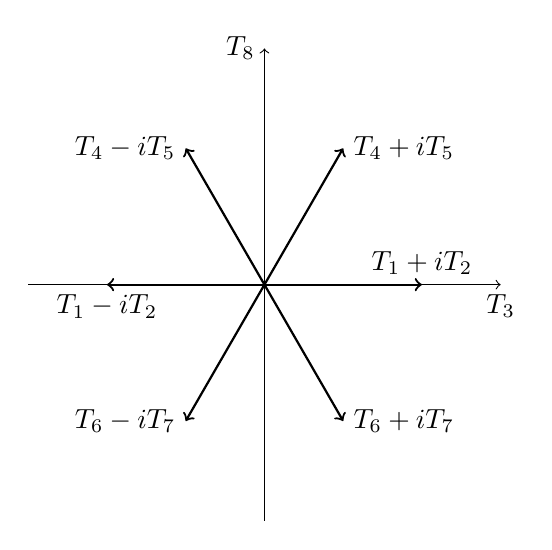
\begin{tikzpicture}
            \draw[->] (-3,0) -- (3,0) node[below] {$T_3$};
            \draw[->] (0,-3) -- (0,3) node[left] {$T_8$};
            \draw[thick,->] (0,0) -- (2,0) node[above] {$T_1+iT_2$};
            \draw[thick,->] (0,0) -- (-2,0) node[below] {$T_1-iT_2$};
            \draw[thick,->] (0,0) -- (1,1.732) node[right] {$T_4+iT_5$};
            \draw[thick,->] (0,0) -- (1,-1.732) node[right] {$T_6+iT_7$};
            \draw[thick,->] (0,0) -- (-1,1.732) node[left] {$T_4-iT_5$};
            \draw[thick,->] (0,0) -- (-1,-1.732) node[left] {$T_6-iT_7$};
        \end{tikzpicture}
% \begin{pspicture}[showgrid=false](-4,-4)(3.5,3.5)\psset{unit=1.3}
%     \psset{linewidth=1.5pt}
%         %Weyl Chambers
%         \pscustom[linewidth=0pt,fillstyle=solid,fillcolor=lightgray]{
%             \psline(0,3)(0,0)
%             \psline(0,0)(2.6,1.5)
%         }
%             \psline[linestyle=dotted,linewidth=1pt](0,-3)(0,3)
%             \psline[linestyle=dotted,linewidth=1pt](-2.6,-1.5)(2.6,1.5)
%             \psline[linestyle=dotted,linewidth=1pt](2.6,-1.5)(-2.6,1.5)

%         %Roots
%         \psline{->}(0,0)(2,0) \psline{->}(0,0)(-2,0)
%         \psline{->}(0,0)(-1,1.732) \psline{->}(0,0)(1,-1.732)
%         \psline{->}(0,0)(1,1.732) \psline{->}(0,0)(-1,-1.732)

%         \uput[225](2,0){$\alpha_1$}
%         \uput[225](-1.7,0){$-\alpha_1$}
%         \uput[225](-1,2){$\alpha_2$}
%         \uput[225](1.5,-1.8){$-\alpha_2$}
%         \uput[225](1.6,2.1){$\alpha_1+\alpha_2$}
%         \uput[225](-0.8,-1.8){$-(\alpha_1+\alpha_2)$}
%         \uput[225](1.3,0.6){$\omega_1$}
%         \uput[225](0.1,1.2){$\omega_2$}

%         %Fundamental Weights
%         \psline[linewidth=1pt]{->}(0,0)(0,1)
%         \psline[linewidth=1pt]{->}(0,0)(0.866,0.5)
% \end{pspicture}
\end{center}

利用$\langle \omega_i|\omega_i\rangle=2/3$以及$\langle \omega_1|\omega_2\rangle=1/3$,在以基本权为基的表示里,内积可以如下计算
\[
	\langle (a,b)|(c,d) \rangle= \frac{2(ac+bd)+(ad+bc)}{3}.
\]
由于Weyl矢量为$\rho=\omega_1+\omega_2=(1,1)$,$\alpha_1=(2,-1)$, $\alpha_2=(-1,2)$,所以对于最高权为$(p,q)$的表示,我们可以计算他的维度如下
\[
	\dim(V_{pq})=\frac{\langle \rho+\lambda|\alpha_1\rangle}{\langle \rho|\alpha_1\rangle}\frac{\langle \rho+\lambda|\alpha_2\rangle}{\langle \rho|\alpha_2\rangle}\frac{\langle \rho+\lambda|\alpha_1+\alpha_2\rangle}{\langle \rho|\alpha_1+\alpha_2\rangle},
\]
其中$\langle \rho|\alpha_1\rangle=\langle \rho|\alpha_2\rangle=1$以及
\[
\langle \lambda|\alpha_1\rangle=p,\quad \langle \lambda|\alpha_2\rangle=q,
\]
所以
\[
	\dim(V_{pq})=\frac{1+p}{1}\frac{1+q}{1}\frac{p+q+2}{2}=\frac{1}{2}(p+1)(q+1)(p+q+2).
\]

\section{不可约表示的张量积}

对于Lie群的表示,$(\rho,V)$和$(\pi,W)$的张量积可以定义为
\[
	(\rho\otimes\pi)(g)(v\otimes w)=(\rho(g)v)\otimes(\pi(g)w),
\]
假设$g=\exp(tX)$,将其在$t=0$上求导就得到了
\[
	(\rho_*(X)v)\otimes w+ v \otimes (\mu_*(X)w),
\]
于是我们定义,两个Lie代数的表示$(\rho,V)$和$(\pi,W)$的张量积为
\[
	(\rho\otimes\pi)(X)(v\otimes w)=(\rho(X)v)\otimes w+ v \otimes (\pi(X)w).
\]
或者记作
\[
	X(|v\rangle\otimes|w\rangle)=X|v\rangle\otimes|w\rangle+|v\rangle\otimes X|w\rangle.
\]
不难检验$(\rho\otimes\pi)([X,Y])=[(\rho\otimes\pi)(X),(\rho\otimes\pi)(Y)]$.

\para 设$(\rho,V)$和$(\pi,W)$是$\lag$的两个不可约表示,我们已经知道分解
\[
	V=\bigoplus_{\lambda\in\Omega_\rho} V_\lambda,\quad W=\bigoplus_{\mu\in\Omega_\pi} W_\mu,
\]
所以
\[
	V\otimes W=\bigoplus_{\lambda\in\Omega_\rho}\bigoplus_{\mu\in\Omega_\pi} V_\lambda\otimes W_\mu,
\]

任取矢量$|\lambda\rangle\in V_\lambda$和$|\mu\rangle\in W_\mu$,我们有
\[
	h|\lambda,\mu\rangle=(\lambda(h)+\mu(h))|\lambda,\mu\rangle,
\]
其中$|\lambda,\mu\rangle=|\lambda\rangle\otimes |\mu\rangle$,因此$\lambda+\mu$是这个张量积表示的一个权,而且$V_\lambda\otimes W_\mu \subset (V\otimes W)_{\lambda+\mu}$. 所以
\[
	\bigoplus_{\lambda\in\Omega_\rho}\bigoplus_{\mu\in\Omega_\pi} V_\lambda\otimes W_\mu\subset \bigoplus_{\gamma\in \Omega_{\rho\otimes\pi}} (V\otimes W)_{\gamma}\subset V\otimes W,
\]
于是$\Omega_{\rho\otimes\pi}=\Omega_{\rho}+\Omega_{\pi}:=\{\lambda+\mu\,:\,\lambda\in\Omega_\rho,\mu\in\Omega_\pi\}$,以及
\[
	(V\otimes W)_{\gamma}=\bigoplus_{\lambda+\mu=\gamma}V_\lambda\otimes W_\mu.
\]
这样我们就得到了两个不可约表示张量积全部的权。

\para 一般而言,表示$(\rho\otimes\pi,V\otimes W)$并不是不可约的,但是由于我们的Lie代数是半单的,所以这是可以完全分解的。由上节的大定理,分解出来的不可约表示都唯一由他的最高权决定,而最高权是那些基本权的非负系数线性组合。所以现在我们的任务就是找到这个张量表示中所有可能的最高权,每一个最高权确定了一个不可约表示。

举个例子,$\mathfrak{sl}(2,\cc)$不可约表示所有可能的最高权是自然数或者半正整数$j$,此时的权为$\{-j$, $-j+1$, $\cdots$, $j-1$, $j\}$.

考虑$\mathfrak{sl}(2,\cc)$在$V\otimes W$上的表示,在$V$和$W$上表示的最高权分别是$j_1$和$j_2$,那么现在可能的权就是$m_1+m_2$,其中$m_i\in\{-j_i$, $\cdots$, $j_i\}$,最高权应该保证$m_1+m_2\geq 0$,所以可能的组合就是$\{|j_1-j_2|$, $|j_1-j_2|+1$, $\cdots$, $j_1+j_2-1$, $j_1+j_2\}$. 因此我们就应该分解到这些最高权对应的不可约表示上面去。

\para 考虑$\mathfrak{sl}(3,\cc)$的例子,他的基本权和根都在上节的图上了。由于Weyl矩阵写作
\[
	A=\begin{pmatrix}
	2&-1\\
	-1&2\\
	\end{pmatrix}.
\]
所以在以基本权的基下,我们有$\alpha_1=(2,-1)$, $\alpha_2=(-1,2)$,还有一个正根是他们的和$\alpha_1+\alpha_2=(1,1)$,剩下的三个根就是这三个根的相反。对于最高权为$(1,0)$的表示,此时可能的权有$(1,0)$和$(-1,1)$. 

考虑最高权为$(1,0)$和$(1,0)$两个表示的张量基$(1,0)\otimes (1,0)$,可能的最高权就只有$(2,0)$和$(0,1)$,用Young图表示,这就是在说
\[
\Yvcentermath1
\yng(1)\otimes \yng(1)=\yng(2)\oplus\yng(1,1).
\]

\para 下面我们用不可约表示的最高权来代表该表示,用$\Omega_{+}$来记所有的dominant weight的集合,这样,我们应该有分解
\[
	\lambda\otimes \mu =\bigoplus_{\nu\in \Omega_{+}}\mathcal{N}_{\lambda\mu}^\nu \nu,
\]
其中$\mathcal{N}_{\lambda\mu}^\nu$是一个自然数,代表分解出来对于最高权为$\nu$的不可约表示的重数。

\para 显然的是,比如
\[
	\mathcal{N}_{\lambda 0}^\nu=\delta_\lambda^\nu
\]

To be continued.

\section{$\operatorname{sl}(n,\cc)$的不可约表示的直接构造}

上面讲了太多的一般的理论了,这里来直接构造$\mathfrak{sl}(n,\cc)$的不可约表示,这并不是一个简单的事情。直接构造在绝大多数情况下,都是很难很难的事情,很考验基本功和天分,乃至于是考验灵感。这节的构造来自于Weyl.%而揭示了$S_n$与$\operatorname{GL}(n)$不可约表示的联系的,又是一个熟悉的名字,Schur.

\para 考虑$V^{\otimes n}=V\otimes\cdots \otimes V$,即自己张量自己$n$次。设$\varphi\in \operatorname{GL}(V)$,那么我们可以诱导出一个新的线性映射$\Phi:V^{\otimes n}\to V^{\otimes n}$通过
\[
	\Phi : e_{i_1}\otimes\cdots\otimes e_{i_n}\mapsto \varphi e_{i_1}\otimes\cdots\otimes \varphi e_{i_n},
\]
其中$\{e_i\}$是$V$的一组基,不难检验,上面的诱导并不依赖于基的选取。

考虑表示的情况,设$\varphi=\rho(\exp(tX))$,$X\in \lag$,那么它诱导了一个映射
\[
	e_{i_1}\otimes\cdots\otimes e_{i_n}\mapsto \rho(\exp(tX)) e_{i_1}\otimes\cdots\otimes \rho(\exp(tX)) e_{i_n},
\]
然后再对$t$在$t=0$处求导,即得到了$\lag$的一个表示$\pi$,满足
\[
	\pi(X):e_{i_1}\otimes\cdots\otimes e_{i_n}\mapsto \sum_{k=1}^ne_{i_1}\otimes\cdots \otimes Xe_{i_k}\otimes \cdots\otimes e_{i_n}.
\]
我们后面构造$\operatorname{sl}(n,\cc)$的表示即是通过这样的张量积来构造。

\para 设$V$是一个矢量空间,以及有一族矢量$\{v_i\in V\,:\, 1\leq i \leq k\}$,那么我们可以定义这样一个完全对称的运算(即算式里面两两对换因子结果不变)
\[
	v_1\cdot v_2\cdots v_{k-1}\cdot v_k,
\]
它对每一个$v_i$都线性。比如对于$k=2$的情况,可以构造为
\[
	v\cdot w= \frac{1}{2}\left(v\otimes w+w\otimes v\right).
\]
至于更高的$k$,也可以通过张量积来定义。后面我们略去这个运算的符号。

设$V$的一组基为$\{e_1,\cdots,e_n\}$,那么所有
\[
	e_{i_1}e_{i_2}\cdots e_{i_{k-1}}e_{i_k}
\]
就张成了一个线性空间,记作$\sym^k(V)$. 这个空间的维数是
\[
	\dim (\sym^{k}(V))={\binom {n+k-1}{k}}
\]

\para 类似地,我们可以定义出一个完全反对称的运算(即算式里面每次两两对换因子结果都会多个负号)
\[
	v_1\wedge v_2\wedge \cdots \wedge v_k,
\]
它对每一个$v_i$都线性,比如对于$k=2$的情况,可以构造为
\[
	v\wedge w= \frac{1}{2}\left(v\otimes w-w\otimes v\right).
\]
至于更高的$k$,也可以通过张量积来定义。

设$V$的一组基为$\{e_1,\cdots,e_n\}$,那么所有
\[
	e_{i_1}\wedge \cdots \wedge e_{i_k}
\]
就张成了一个线性空间,记作$\Lambda^k(V)$. 注意到,当$k>n$的时候,上式中肯定存在某个重复的$e_{i_j}$,由于
\[
	e_{i_1}\wedge e_{i_1}=- e_{i_1}\wedge e_{i_1},
\]
所以自然为零。因此如果$k>n$,$\Lambda^k(V)=0$.

对于$k\leq n$的情况,这个空间的维数是
\[
	\dim (\Lambda^{k}(V))={\binom {n}{k}},
\]
所以$\dim (\Lambda^{k}(V))=\dim (\Lambda^{n-k}(V))$.

\para 由于不管$\sym^k(V)$还是$\Lambda^{k}(V)$,他们都可以通过张量积来定义,于是Lie代数在$V$上的表示类似诱导了
\[
	\pi(X):e_{i_1}\cdots e_{i_k}\mapsto \sum_{k=1}^ne_{i_1}\cdots  Xe_{i_k} \cdots e_{i_k},
\]
\[
	\pi(X):e_{i_1}\wedge\cdots\wedge e_{i_k}\mapsto \sum_{k=1}^ne_{i_1}\wedge\cdots \wedge Xe_{i_k}\wedge \cdots\wedge e_{i_k}.
\]

\para 上一节我们已经看到了,对于$\mathfrak{sl}(N,\cc)$,基可以选取为
\[
	\begin{cases}
		H_{ij}=E_{ii}-E_{jj},\\
		E_{ij}=E_{ij},\\
		F_{ij}=E_{ji},
	\end{cases}
\]
以及他们的对易关系
\[
	[H_{ij},E_{ij}]=2 E_{ij},\quad [H_{ij},F_{ij}]=-2 F_{ij},\quad [E_{ij},F_{ij}]=H_{ij}.
\]
其中,对应于单根$\alpha_i$的$h^i=H_{i,i+1}$.

\para 考虑$N=2$的情况,此时
\[
	H=\begin{pmatrix}
	1&0\\
	0&-1
	\end{pmatrix},\quad E=\begin{pmatrix}
	0&1\\
	0&0
	\end{pmatrix},\quad F=\begin{pmatrix}
	0&0\\
	1&0
	\end{pmatrix}
\]
设$\cc^2$的基为$x=(1,0)^T$和$y=(0,1)^T$,则
\[
	\begin{cases}
	Hx=x,\\
	Hy=-y,
	\end{cases}\quad 
	\begin{cases}
	Ex=0,\\
	Ey=x,
	\end{cases}\quad 
	\begin{cases}
	Fx=y,\\
	Fy=0.
	\end{cases}
\]
这个表示被称为标准表示(即定义$\mathfrak{sl}(2,\cc)$的表示)。

所以在$\sym^n(\cc^2)$里
\[
	H(x^ky^{n-k})=kx^ky^{n-k}-(n-k)x^ky^{n-k}=(n-2k)x^ky^{n-k},
\]
换而言之,$\sym^n(\cc^2)$张成了对应$H$最高本征值\footnote{物理上惯常用的是$H/2$,所以本征值为一半。}为$n$的那个不可约表示,维度很容易计算,是$n+1$.

\para 考虑$N=3$的情况,依然是考虑标准表示。由于$H_{ij}$本来就是对角化的,所以此时的权矢量就是$\cc^3$的基,$x=(1,0,0)^T$, $y=(0,1,0)^T$和$y=(0,0,1)^T$. 考虑$h^1=e_1$以及$h^2=e_2$,我们有
\[
	\begin{cases}
	h^1x=x,\\
	h^1y=-y,\\
	h^1z=0,
	\end{cases}\quad 
	\begin{cases}
	e^1x=0,\\
	e^1y=x,\\
	e^1z=0,
	\end{cases}\quad 
	\begin{cases}
	f^1x=y,\\
	f^1y=0,\\
	f^1z=0.
	\end{cases}
\]
\[
	\begin{cases}
	h^2x=0,\\
	h^2y=y,\\
	h^2z=-z,
	\end{cases}\quad 
	\begin{cases}
	e^2x=0,\\
	e^2y=0,\\
	e^2z=y,
	\end{cases}\quad 
	\begin{cases}
	f^2x=0,\\
	f^2y=z,\\
	f^2z=0.
	\end{cases}
\]

记$x=|\lambda_1\rangle$, $y = |\lambda_2 \rangle$, $z = |\lambda_3 \rangle$,由于
\[
	h^1|\lambda_1\rangle=|\lambda_1\rangle,\quad h^2|\lambda_1\rangle=0,
\]
所以由式\eqref{dynkin},我们就计算出$\lambda_1$的Dynkin指标为$\lambda_1=(1,0)=\omega_1$,类似地,可以计算出
\[
	\lambda_2=(-1,1)=\omega_2-\omega_1,\quad \lambda_3=(0,-1)=-\omega_2.
\]
它对应于最高权为$(1,0)$的那个不可约表示。作图如下:

\begin{center}
\begin{pspicture}[showgrid=false](-4,-4)(3.5,3.5)\psset{unit=1.3}
    \psset{linewidth=1.5pt}
        \psline[linestyle=dotted,linewidth=1pt](0,-2)(0,2)
        \psline[linestyle=dotted,linewidth=1pt](-2.1,-1.3)(2.1,1.3)
        \psline[linestyle=dotted,linewidth=1pt](2.1,-1.3)(-2.1,1.3)

        \uput[225](1.3,0.6){$\omega_1$}
        \uput[225](-1.0,0.7){$\omega_2-\omega_1$}
        \uput[225](-0.1,-1){$-\omega_2$}

        \psline[linewidth=1pt]{->}(0,0)(0,-1)
        \psline[linewidth=1pt]{->}(0,0)(0.866,0.5)
        \psline[linewidth=1pt]{->}(0,0)(-0.866,0.5)
        \psline[linestyle=dotted,linewidth=1.5pt](0,-1)(0.866,0.5)
        \psline[linestyle=dotted,linewidth=1.5pt](0,-1)(-0.866,0.5)
        \psline[linestyle=dotted,linewidth=1.5pt](0.866,0.5)(-0.866,0.5)
\end{pspicture}
\end{center}

这就是标准表示的三个权,其中最高权为$(1,0)$,物理上有时候会叫他夸克表示,因为是三维的,有时候也记作$3$。类似$\mathfrak{sl}(2)$的情况,表示$\sym^a(\cc^3)$包含权$(a,0)$,而且这个权无简并,注意到,此时$\sym^a(\cc^3)$不一定是不可约的。由于$\cc^3=\Lambda^1(\cc^3)$,所以$\sym^a(\cc^3)=\sym^a(\Lambda^1(\cc^3))$.

\para 接着我们考虑$\mathfrak{sl}(3,\cc)$在$\Lambda^2(\cc^3)$上面的表示,注意到,此时$\dim (\Lambda^2(\cc^3))=3$,和标准表示的维度一样,但是这个表示和标准表示并不一样。

记$\bar{x}=y\wedge z$,$\bar{y}=x\wedge z$和$\bar{z}=x\wedge y$,于是
\[
	h^1\bar{x}=(h^1y)\wedge z+y\wedge (h^1z)=-y\wedge z=-\bar{x},
\]
类似容易计算得
\[
	\begin{cases}
	h^1\bar{x}=-\bar{x},\\
	h^1\bar{y}=\bar{y},\\
	h^1\bar{z}=0,
	\end{cases}\quad 
	\begin{cases}
	e^1\bar{x}=\bar{y},\\
	e^1\bar{y}=0,\\
	e^1\bar{z}=0,
	\end{cases}\quad 
	\begin{cases}
	f^1\bar{x}=0,\\
	f^1\bar{y}=\bar{x},\\
	f^1\bar{z}=0.
	\end{cases}
\]
\[
	\begin{cases}
	h^2\bar{x}=0,\\
	h^2\bar{y}=-\bar{y},\\
	h^2\bar{z}=\bar{z},
	\end{cases}\quad 
	\begin{cases}
	e^2\bar{x}=0,\\
	e^2\bar{y}=\bar{z},\\
	e^2\bar{z}=0,
	\end{cases}\quad 
	\begin{cases}
	f^2\bar{x}=0,\\
	f^2\bar{y}=0,\\
	f^2\bar{z}=\bar{y}.
	\end{cases}
\]

记$\bar{x}=|\lambda_1\rangle$, $\bar{y} = |\lambda_2 \rangle$, $\bar{z} = |\lambda_3 \rangle$,由于
\[
	h^1|\lambda_1\rangle=-|\lambda_1\rangle,\quad h^2|\lambda_1\rangle=0,
\]
所以由式\eqref{dynkin},我们就计算出$\lambda_1$的Dynkin指标为$\lambda_1=(-1,0)=-\omega_1$,类似地,可以计算出
\[
	\lambda_2=(1,-1)=\omega_1-\omega_2,\quad \lambda_3=(0,1)=\omega_2.
\]
它对应于最高权为$(0,1)$的那个不可约表示。作图如下:

\begin{center}
\begin{pspicture}[showgrid=false](-4,-4)(3.5,3.5)\psset{unit=1.3}
    \psset{linewidth=1.5pt}
        \psline[linestyle=dotted,linewidth=1pt](0,-2)(0,2)
        \psline[linestyle=dotted,linewidth=1pt](-2.1,-1.3)(2.1,1.3)
        \psline[linestyle=dotted,linewidth=1pt](2.1,-1.3)(-2.1,1.3)

        \uput[225](-0.9,-0.5){$-\omega_1$}
        \uput[225](1.7,-0.5){$\omega_1-\omega_2$}
        \uput[225](0.1,1.3){$\omega_2$}

        \psline[linewidth=1pt]{->}(0,0)(0,1)
        \psline[linewidth=1pt]{->}(0,0)(-0.866,-0.5)
        \psline[linewidth=1pt]{->}(0,0)(0.866,-0.5)
        \psline[linestyle=dotted,linewidth=1.5pt](0,1)(-0.866,-0.5)
        \psline[linestyle=dotted,linewidth=1.5pt](0,1)(0.866,-0.5)
        \psline[linestyle=dotted,linewidth=1.5pt](-0.866,-0.5)(0.866,-0.5)
\end{pspicture}
\end{center}

这被称为标准表示的伴随表示,最高权为$(0,1)$,物理上有时候会叫他反夸克表示,它是三维的但是要区别标准标识,有时候也记作$\bar{3}$。

类似标准表示的情况,表示$\sym^b(\Lambda^2(\cc^3))$中包含权$(0,b)$,且无简并。

\para 综上,对于$\mathfrak{sl}(3,\cc)$而言,表示
\[
	W_{(a,b)}=\sym^a(\Lambda^1(\cc^3))\otimes\sym^b(\Lambda^2(\cc^3)).
\]
中存在我们希望的权$(a,b)$,并且无简并。所以$(a,b)$对应的不可约表示$V_{(a,b)}$应该是上面这个表示$W_{(a,b)}$的子表示。

\para 类似地,为了构造出$\mathfrak{sl}(N,\cc)$的以$(\lambda_1,\cdots,\lambda_{N-1})$为最高权的不可约表示,我们需要构造出最高权为$(0,0,\cdots,1,\cdots,0)$的不可约表示,然后通过对称化得到包含权$(0,0,\cdots,\lambda_i,\cdots,0)$的表示。

容易验证,对应于最高权$(0,0,\cdots,1,\cdots,0)$的不可约表示就是$\Lambda^i\bigl(\cc^N\bigr)$,它由
\[
	v_{n_1}\wedge \cdots \wedge v_{n_i}
\]
张成,其中$\{v_i\,:\, 1\leq i \leq N\}$是$\cc^N$的标准基。可以假设$\{n_k\}$是递增的,这组基也构成了$\{h^i\}$的共同本征矢量。由于
\[
	e^i:v_{j+1}\to 
	\begin{cases}
		\delta_{ij}v_j,& j>0;\\
		0,& j=0.
	\end{cases}
\]
所以
\[
	e^j(v_{n_1}\wedge \cdots \wedge v_{n_i})=\sum_{k=1}^i\delta_{n_k+1,j}v_{n_1}\wedge \cdots \wedge v_{n_k-1}\wedge\cdots \wedge v_{n_i},
\]
上式求和中最多只能存在一项,因为$\{n_i\}$两两不相同。如果$v_{n_1}\wedge \cdots \wedge v_{n_i}$对任意的$\{e_j\,:\, 1\leq j\leq i\}$都成立
\[
	e^j(v_{n_1}\wedge \cdots \wedge v_{n_i})=0,
\]
于是只可能$n_{k}=k$,即$v_{1}\wedge \cdots \wedge v_{i}$是单项式中唯一那个权矢量使得任意的上升算符$e_i$作用在上面都为$0$.

对于多项式的情况,由于在$e^i$作用下每一项都产生变化,原本不同的不可能变成相同的,所以并不会出现在所有上升算符$e_i$作用在上面都为$0$. 因此$v_{1}\wedge \cdots \wedge v_{i}$是唯一的最高权。因此是一个不可约表示,维数是${\binom {n}{i}}$.

于是,包含权$(0,0,\cdots,\lambda_i,\cdots,0)$的表示就是
\[
	\sym^{\lambda_i}\left(\Lambda^i\bigl(\cc^N\bigr)\right),
\]
最后,包含最高权$(\lambda_1,\cdots,\lambda_{N-1})$的一个表示就是
\[
\begin{split}
	W_{(\lambda_1,\cdots,\lambda_{N-1})}&=\sym^{\lambda_1}\left(\Lambda^1\bigl(\cc^N\bigr)\right)\otimes \cdots \otimes \sym^{\lambda_i}\left(\Lambda^i\bigl(\cc^N\bigr)\right)\otimes \cdots \otimes \sym^{\lambda_{N-1}}\left(\Lambda^{N-1}\bigl(\cc^N\bigr)\right)\\
	&=\bigotimes_{i=1}^{N-1}\sym^{\lambda_i}\left(\Lambda^i\bigl(\cc^N\bigr)\right).
\end{split}
\]
我们需要的不可约表示$V_{(\lambda_1,\cdots,\lambda_{N-1})}$是$W_{(\lambda_1,\cdots,\lambda_{N-1})}$的一个子表示。

$W_{(\lambda_1,\cdots,\lambda_{N-1})}$的维度是可以直接计算的
\[
	\dim\left(V_{(\lambda_1,\cdots,\lambda_{N-1})}\right)=\prod_{i=1}^{N-1}{\binom {\binom{N}{i}+\lambda_i-1}{\lambda_i}}.
\]
因为这个表示不是不可约的,所以维度要比不可约表示的维度要大。

\para 往Young图中填数字可以用来确定权矢量。比如对于最高权为$(2,0,2)$的$\mathfrak{sl}(4,\cc)$的表示,
\[
	W_{(2,0,2)}=\sym^{2}\left(\Lambda^1\bigl(\cc^4\bigr)\right)\otimes \sym^{2}\left(\Lambda^3\bigl(\cc^4\bigr)\right),
\]
它对应的Young图为
\[
	\yng(4,2,2)
\]
注意到,三行的两列,一行的有两列,前者对应于$\sym^{2}\left(\Lambda^3\bigl(\cc^4\bigr)\right)$,后者对应于$\sym^{2}\left(\Lambda^1\bigl(\cc^4\bigr)\right)$. 对每一列往里面填入数字我们对应于一个$\Lambda^3\bigl(\cc^4\bigr)$里面的权矢量,比如
\[
\Yvcentermath1
	\young(i,j,k)\quad \mapsto \quad v_i\wedge v_j \wedge v_k,
\]
由于$i$, $j$和$k$互换位置只差个负号,所以我们还能假设$i<j<k$. 那么比如
\[
\Yvcentermath1
	\young(1224,33,44) \quad \mapsto \quad (v_1\wedge v_3 \wedge v_4)(v_2\wedge v_3 \wedge v_4)\otimes (v_2 v_4),
\]
就确定了一个权矢量。按照我们的习惯,填数字的时候,每一列的数字都是递增的,如果一列中出现了两个相同的数字,那么这个权矢量就是$0$. 但注意到,我们并没有对每一行的数字进行限制,如果出现两列行数相同的情况,则该两列互调对权矢量并不产生影响,那么可以任意选定一个顺序,比如字典序,来固定一个数字填法。

Young图填数字得到的表称为Young表。

\para 既然每一个Young表确定了一个权矢量,那么我们如何从这个Young表中得到权呢?或者问的更广一些,怎么定义Young表的运算呢?

注意到,Young表每一个小方块与其他小方块都是通过张量积来进行连接的,所以任何一个Lie代数里面的元素作用在Young表上,都表现为分别作用在每一个小方块上,然后加起来。

以$h^i$为例,我们来计算给定Young表的权。依然还是使用式\eqref{dynkin},我们就是要计算
\[
\Yvcentermath1
	h^i \,\young(1224,33,44)= \lambda^i \,\young(1224,33,44),
\]
中的$\lambda^i$,由于$\Yvcentermath1 h^i\young(j)=\delta_{ij}-\delta_{i+1,j}$,所以
\[
	\lambda_i = \# i - \# (i+1),
\]
其中$\# i$表示表中数字$i$出现的个数,所以
\[
	\lambda= \sum_{i=1}^{N-1} \lambda_i \omega_i =\sum_{i=1}^{N-1} \left(\# i - \# (i+1)\right)\omega_i,
\]
补充定义$\omega_0=\omega_N=0$之后,上式可以改写为
\[
	\lambda=\sum_{i=1}^{N-1} (\# i)\omega_i - \sum_{i=2}^N(\# i)\omega_{i-1}=\sum_{i=1}^{N} (\# i)\left(\omega_i - \omega_{i-1}\right),
\]
记$\gamma_i=\omega_i - \omega_{i-1}$,则上式最后就写成$\lambda=\sum_{i=1}^{N} (\# i)\gamma_i$,即每一个$\Yvcentermath1 \young(i)$赋予一个$\gamma_i$,最后再全部加起来即可。

所以
\[
\Yvcentermath1
	\young(1224,33,44)
\]
对应的权$\lambda = \gamma_1+2\gamma_2+2\gamma_3+3\gamma_4=-\omega_1-\omega_3=(-1,0,-1)$.

\para 反过来,如何从一个权来构造一个Young表呢?考虑最高权$\lambda=(\lambda_1$ ,$\cdots$ ,$\lambda_{N-1})=\{l_1$ ,$\cdots$ ,$l_{N-1}\}$,我们有如下的方程
\[
	\lambda_i=\# i - \# (i+1),
\]
所以
\[
	\# (i+1)=\# i-\lambda_i=\#(i-1)-(\lambda_i+\lambda_{i-1})=\cdots=\# 1-\sum_{n=1}^{i}\lambda_n,
\]
所以在补充定义$l_N=0$的情况下,可以写作
\[
	\# i = \# 1-\sum_{n=1}^{i-1}\lambda_n=\# 1 - l_1 + l_i.
\]

此外,由于所有的格子数正好等于$\sum_{i=1}^{N-1}l_i=\sum_{i=1}^{N}l_i$,同时也正好等于所有的数字个数之和,故
\[
	\sum_{i=1}^{N}l_i = \sum_{i=1}^N \#i,
\]
或者
\[
	 \sum_{i=1}^{N}l_i = \sum _{i=1}^N (\# 1 - l_1 + l_i)=N(\# 1 - l_1)+\sum_{i=1}^{N}l_i,
\]
所以$\# 1=l_1$,然后
\[
	\# i = \# 1 - l_1 + l_i= l_i,
\]
这就解出了最高权的Young表中所有数字出现的个数,$\Yvcentermath1 \young(i)$出现的次数刚好就是第$i$行的格子数。由于每一列的数字都是递增的假设,我们可以断言,最高权的Young表,第$i$行全都是$\Yvcentermath1 \young(i)$. 比如最高权为$(2,0,2)$的Young表为
\[
\Yvcentermath1
	\young(1111,22,33)
\]
所以,我们也就再次得到了,在我们的构造中,最高权不可能是简并的。

对于非最高权$\lambda=\{l_1,\cdots,l_{N-1}\}$的情况,设最高权为$\lambda_m=\{l'_1,\cdots,l'_{N-1}\}$,则类似地可以得到方程
\[
	 \sum_{i=1}^{N}l'_i = \sum _{i=1}^N (\# 1 - l_1 + l_i)=N(\# 1 - l_1)+\sum_{i=1}^{N}l_i,
\]
所以
\[
	\# 1=l_1+\frac{1}{N}\sum_{n=1}^N(l'_n-l_n),
\]
以及
\[
	\# i = l_i + \frac{1}{N}\sum_{n=1}^N(l'_n-l_n).
\]

\para 即使确定了每一个$\Yvcentermath1 \young(i)$出现的次数,Young表的填写方式也可能是千奇百怪的,比如在$\mathfrak{sl}(3,\cc)$在最高权为$(1,1)$的表示中,权矢量
\[
\Yvcentermath1
	\young(12,3)\quad \text{,}\quad \young(13,2) \quad \text{and}\quad \young(21,3)
\]
确定的权是相同的。这就可能出现简并的情况。

更糟糕的是,对一个权$\lambda$,我们构造的表示$W_\lambda$不一定是不可约的,它是一些不可约表示的直和,我们只想要其中对应最高权$\lambda$的那个不可约表示$V_\lambda$。但是在求权矢量的时候,其他不可约表示的部分也参杂了进来。这就意味着,我们随便画一个Young表,它可能不是我们想要的不可约表示$V_\lambda$的一个权矢量。乃至,我们为了构造一个合适的权矢量,只能适当线性组合那些Young表。

比如考虑矢量
\begin{equation}
\Yvcentermath1
	v=\young(21,3)\,+\,\young(13,2)\,-\,\young(12,3)
\end{equation}
容易计算$e^1v=e^2v=0$,因此$v$应该是某个不可约表示的最高权。它的权容易计算是$(0,0)$,所以这是一个平凡表示的最高权。

因此,对应于最高权为$(1,1)$表示的$(0,0)$权矢量应该被构造成
\[
\Yvcentermath1
	\young(13,2)\,+\,\young(12,3)\quad \text{and}\quad \young(21,3)\,+\,\young(12,3)
\]
这才是正确的情况。此时$(0,0)$是双重简并的。

\para 构造权矢量最安全的方式还是从最高权矢量开始使用$\{f^i\}$往下降得到,毕竟最高权矢量的Young表我们是已经知道了的。举个例子,考虑最高权对应的Young表
\[
\Yvcentermath1
	\young(11,2)
\]
$\{f^i\}$的作用为
\[
	f^i:v_{j}\to 
	\begin{cases}
		\delta_{ij}v_{j+1},& j>0;\\
		0,& j=N.
	\end{cases}
\]
为了得到权$(0,0)$,我们需要数字$1$, $2$, $3$各一个,一种方式可以这样:
\[
\Yvcentermath1
	\young(11,2)\,\xrightarrow{f^2}\,\young(11,3)\,\xrightarrow{f^1}\,\young(12,3)\,+\,\young(21,3)
\]
另一条路线可以这样选择
\[
\Yvcentermath1
	\young(11,2)\,\xrightarrow{f^1}\,\young(12,2)\,\xrightarrow{f^2}\,\young(12,3)\,+\,\young(13,2)
\]
所以$(0,0)$是双重简并的。

{\thm 在Young表中,每一行不减,每一列递增的Young表被称作准标准Young表。在$\mathfrak{sl}(N,\cc)$不可约表示中,对应于权$\lambda$的权子空间的个数正好等于权为$\lambda$的准标准Young表的个数。\endthm}

注意,这里的准标准Young表对应的权矢量不一定是我们不可约表示的权矢量,这是一个组合学意义上的命题。但是,一种特例下,我们是可以知道权矢量的,就是权子空间无简并,此时准标准Young表正好确定了那个权矢量。

\para 举个例子,$\mathfrak{sl}(4,\cc)$对应最高权$(2,0,2)$的不可约表示$V_{(2,0,2)}$,它的一个准标准Young表是
\[
	\young(1224,33,44)
\]
它的权前面计算过是$\gamma_1+2\gamma_2+2\gamma_3+3\gamma_4=-\omega_1-\omega_3=(-1,0,-1)$,而且由于每一行都是不减的,所以$(-1,0,-1)$是不可约表示$V_{(2,0,2)}$的一个权。他与
\[
	\young(1234,23,44)
\]
构成可能的两个准标准Young表,所以权$(-1,0,-1)$的简并为$2$.

\para 为了正确构造$\mathfrak{sl}(n,\cc)$的不可约表示,我们需要类似于式(\theequation)的矢量从我们的构造中消去,为此,我们引入如下运算
\[
	(v_1\wedge \cdots \wedge v_p)\cdot (w_1\wedge\cdots \wedge w_q)=\sum_{i=1}^p(v_1\wedge\cdots \wedge v_{i-1}\wedge w_1 \wedge v_{i+1}\wedge \cdots \wedge v_p)\cdot (v_i\wedge w_2\wedge\cdots \wedge w_q),
\]
这个式子要假设对任意的$p$和$q$都成立,用Young表来表述的话,上面的式子就是在说
\[
  \begin{tabular}{ | c | c |}
    \hline
    {\small $v_1$} \\ \hline
    {\small $v_2$} \\ \hline
    {\small $\vdots$} \\ \hline
    {\small $v_p$} \\ \hline
  \end{tabular}
  \cdot
  \begin{tabular}{ | c | c |}
    \hline
    {\small $w_1$} \\ \hline
    {\small $w_2$} \\ \hline
    {\small $\vdots$} \\ \hline
    {\small $w_q$} \\ \hline
  \end{tabular}=
  \sum_{i=1}^p \begin{tabular}{ | c | c |}
    \hline
    {\small $v_1$} \\ \hline
    {\small $v_2$} \\ \hline
    {\small $\vdots$} \\ \hline
    {\small $v_{i-1}$} \\ \hline
    {\small $w_1$} \\ \hline
    {\small $v_{i+1}$} \\ \hline
    {\small $\vdots$} \\ \hline
    {\small $v_p$} \\ \hline
  \end{tabular}
  \cdot
  \begin{tabular}{ | c | c |}
    \hline
    {\small $v_i$} \\ \hline
    {\small $w_2$} \\ \hline
    {\small $\vdots$} \\ \hline
    {\small $w_q$} \\ \hline
  \end{tabular}
\]
就是将第二列中的$w_1$和第二列中的$v_i$互换,然后将所有这种可能性求和。

举个例子,比如
\[
\Yvcentermath1
	\young(2,3)\cdot \young(1) \,=\, \young(1,3)\cdot \young(2)\,+\,\young(2,1)\cdot \young(3) \,=\, \young(1,3)\cdot \young(2)\,-\,\young(1,2)\cdot \young(3)
\]
上面的运算中用到了任意的一列都是反对称的。利用这个式子,我们建立等同
\[
\Yvcentermath1
	\young(21,3) \,=\, \young(12,3) \,-\, \young(13,2)
\]
注意到式(\theequation)现在在这种等同下有
\[
\Yvcentermath1
	v=\young(21,3)\,+\,\young(13,2)\,-\,\young(12,3)= \young(12,3) \,-\, \young(13,2)\,+\,\young(13,2)\,-\,\young(12,3)=0,
\]
这正是我们需要的。

耐心的计算可以证明,所有的非准标准Young表都可以利用上面那种等同,变成一些准标准Young表的线性组合。更进一步地,可以直接计算得到,那些准标准Young表在等同下还是线性无关的。所以按照上面的定理,准标准Young表的个数等于不可约表示的维度,我们也就得到了下面这个定理。

{\thm 在上面那种等同下,对于$\mathfrak{sl}(N,\cc)$的任意dominant weight $\lambda=(\lambda_1$, $\lambda_2$, $\cdots$, $\lambda_{N-1})$,所有准标准Young表构成了不可约表示$V_\lambda$的一组基。\endthm}

用数学一点的语言,就是说在
\[
	W_{(\lambda_1,\cdots,\lambda_{N-1})}=\bigotimes_{i=1}^{N-1}\sym^{\lambda_i}\left(\Lambda^i\bigl(\cc^N\bigr)\right).
\]
模掉所有
\[
	(v_1\wedge \cdots \wedge v_p)\otimes (w_1\wedge\cdots \wedge w_q)-\sum_{i=1}^p(v_1\wedge\cdots \wedge v_{i-1}\wedge w_1 \wedge v_{i+1}\wedge \cdots \wedge v_p)\otimes (v_i\wedge w_2\wedge\cdots \wedge w_q)
\]
生成的理想$I$,就得到了$V_{(\lambda_1,\cdots,\lambda_{N-1})}$,即
\[
	V_{(\lambda_1,\cdots,\lambda_{N-1})}=W_{(\lambda_1,\cdots,\lambda_{N-1})}/I.
\]

注意到当$p=q$的时候,在$I\cap \sym^{\lambda_p}\left(\Lambda^p\bigl(\cc^N\bigr)\right)$实际上由那些
\[
	(v_1\wedge \cdots \wedge v_p) (w_1\wedge\cdots \wedge w_p)-\sum_{i=1}^p(v_1\wedge\cdots \wedge v_{i-1}\wedge w_1 \wedge v_{i+1}\wedge \cdots \wedge v_p) (v_i\wedge w_2\wedge\cdots \wedge w_p)
\]
生成。

\para 从上面的构造,可以看到所有算符作用在Young表上的形式都不变。所以在实际的计算(比如上升和下降算符的作用)中,从准标准Young表出发,一路进行运算,只要将最后的结果中的那些非准标准Young表利用等同将其变成准标准的,我们就得到了最后的结果。

$\mathfrak{sl}(N,\cc)$不可约表示的另一个构造利用了对称群,利用了Young对称化子,这个在附录中予以了阐述。

\para 通过数可能的准标准Young表可以得到不可约表示的维度,或者使用Weyl特征标公式,也可以得到维度。对于$\mathfrak{sl}(N,\cc)$的最高权$\lambda=(\lambda_1,\cdots \lambda_{N-1})$,在谈论Young图的时候,我们把这个变成了$\{l_1$, $\cdots$, $l_{N-1}\}$,其中$l_i=\sum_{k=i}^{N-1}\lambda_k$,再顺便令$l_N=0$,则对于$\mathfrak{sl}(N,\cc)$不可约表示关于这个最高权的维度我们可以通过下式计算:
\[
	\dim(V_\lambda)=\prod_{1\leq i<j\leq N}\left(\frac{l_i-l_j}{j-i}+1\right).
\]

上面这个公式也可以利用Young图来表示,可以说完全是组合学的技巧,当然似乎也可以利用$S_N$与$\operatorname{GL}(N,\cc)$的不可约表示的对偶。考虑Young图
\[
	\yng(2,2)\,,
\]
往第$(i,j)$格里面填入他下面以及右边所有格子的总量,再加上$1$,对于上面的Young图就是
\[
	\young(32,21)\,,
\]
然后定义$h$为里面所有数字之积,即这里是$3\times 2\times 2\times 1=12$.

然后,依旧是那个Young图,往最左上的一个格子里面填上$N$,之后往左就递增1,往下就递减1,得到了
\begin{center}
  \begin{tabular}{ | c | c |}
    \hline
    $N$ & $N+1$  \\ \hline
    $N-1$ & $N$\\
    \hline
  \end{tabular}
\end{center}
然后计算出$F$为里面所有数之积,即这里是$F=(N+1)N^2(N-1)$.

对应于这幅Young图的不可约表示的维度如下确定
\[
	F/h=(N+1)N^2(N-1)/12,
\]
对于$N=3$的情况,此时维度即$6$. 如果利用公式$(p+1)(q+1)(p+q+2)/2$,这里$p=2$, $q=0$,所以依然可以求得$2\times 1\times 3/2=6$.

\clearpage

	\appendix
\noindent \textbf{\huge Appendix}

\cftaddtitleline{toc}{section}{Appendix}{}
\renewcommand{\thepara}{\Alph{section}.\arabic{para}}

\section{Lie群基础}

\para 设$G$为群,单位元记做$e$,群运算记做$\mu:G\times G\to G$,如果$G$是一个光滑流形,且$\mu$是一个光滑映射,则称$G$是一个光滑Lie群。当然可以谈论不怎么光滑的Lie群,但是下面所指的Lie群都是光滑的。记$l_g$是左作用算符,即$l_g=\mu(g,\cdot)$,或者写作$l_gh=gh$,同样,右作用算符记做$r_g$,即$r_gh=hg$.显然这些都是光滑映射。

现在考虑方程$\mu(x,y)=e$,由于$(l_e)_{*e}$是一个恒同映射,所以在$e$附近,按隐函数定理,方程$\mu(x,y)=e$在$e$附近有光滑解,即$y=\nu(x)=x^{-1}$中的逆函数$\nu$在$e$附近光滑,由于$(\nu\circ l_g)(h)=h^{-1}g^{-1}=(r_{g^{-1}}\circ \nu)(h)$,所以逆函数$\nu$处处光滑。

因为Lie群有着光滑流形结构,那么我们就可以对其局部线性化,特别地,单位元附近的局部线性化就构成了Lie代数的内容。

\para 一个Lie群$G$的Lie代数$\lag$就是其单位元处的切空间。
\endpara

由于$l_g$和$r_g$都是$G\to G$的光滑同胚,所以$(l_g)_*$或者$(r_g)_*$就是将光滑切矢量场映射到光滑切矢量场的双射。如果矢量场$X_x$满足$(l_a)_*X_x=X_{ax}$,则称$X$是一个左不变矢量场。对于左不变矢量场$X$而言,由于\footnote{设$f:M\to N$是一个光滑单射,而$X$是$M$上的一个光滑矢量场,则$f_*X:p\mapsto f_{*f^{-1}(p)}X_{f^{-1}(p)}$是$N$上的一个矢量场。因为$(f_*X)g=X(g\circ f)$成立,所以这也是一个光滑矢量场。}$(l_a)_*X:g\mapsto (l_a)_{*a^{-1}g}X_{a^{-1}g}=X_g$,所以$(l_a)_*X=X$.

和任意的矢量场一样,左不变矢量场$X$在$e$处诱导了$\lag$中的元素$X_e$. 反过来,设$X_e\in\lag$,我们可以构造一个左不变矢量场$x\mapsto X_x=(l_{x})_*X_e$,因此我们就建立了Lie代数和左不变矢量场之间的一一对应。

\para 左不变矢量场都是光滑的且完备的。
\endpara

实际上,任取$f\in\calf(G)$以及$g\in G$,我们来看$(Xf)(g)=X_gf=(l_g)_{*}X_ef=X_e(f\circ l_g)$. 取一个在$e$处切矢量为$X_e$的曲线$\sigma$,则
\[
	Xf(g)=\frac{\dd }{\dd t}\bigg|_{t=0}f(g\sigma(t))=\frac{\dd }{\dd t}\bigg|_{t=0}f\circ \mu(g,\sigma(t)),
\]
是一个光滑函数,所以左不变矢量场都是光滑矢量场。至于完备性,设$\sigma$是左不变矢量场$X$的积分曲线,则$l_g\circ \sigma$也是$X$的积分曲线,这就使得我们可以把一条局部积分曲线拼到无穷远,这就是说$X$是完备的。

\para 设$X$是左不变矢量场,因为$X$是完备的,所以他诱导的单参数变换群$\{\sigma^X_t\}$在整个Lie群上是有定义的,特别地,在单位元上,我们定义$\exp(t,X):=\sigma^X_t(e)$,其中$X$是左不变矢量场,因为左不变矢量场一一对应着Lie代数,所以也可以说$X\in \lag$. 同样,对固定的$X$,映射$\exp(t,X)$对改变的$t$就构成了$G$的一个子群,这被称为单参子群。由积分曲线的存在唯一性,我们也得到了单参子群与Lie代数的一一对应关系。

{\pro 设$f:G\to G$是一个微分同胚,我们有$f_*[X,Y]=[f_*X,f_*Y]$,若$f=l_a$,那么我们立刻就得到了左不变矢量场的对易子也是左不变的。因此对于Lie代数来说,他继承了切矢量场的Lie括号$[\star,\star]:\lag\times \lag\to \lag$,这是一个二元线性运算,所以Lie代数确实是一个代数。\endpro}

通过直接的计算,Lie代数上满足:

\no{1} $[X,Y]=-[Y,X]$,

\no{2} $[X,[Y,Z]]+[Y,[Z,X]]+[Z,[X,Y]]=0$.

第一条反对称性从矢量场的$[X,Y]=XY-YX$来看是显然的。而第二条称为Jacobi恒等式,直接计算即可验证。可以如下记忆Jacobi恒等式,$X$, $Y$和$Z$的三种右手方向构成的置换和为$0$,或者说,$[X_i,[X_j,X_k]]$中$ijk$是$123$的偶置换。

\para Lie代数上的双线性映射$f$如果满足$f([X,Y])=[f(X),Y]+[X,f(Y)]$,则$f$被称为一个导子。\endpara

在Lie代数上我们可以找到一个自然的导子。适当改写Jacobi恒等式,我们可以得到$[X,[Y,Z]]=[[X,Y],Z]+[Y,[X,Z]]$,如果记$\ad(X):Y\mapsto [X,Y]$,于是
\[
	\ad(X)([Y,Z])=[\ad(X)Y,Z]+[Y,\ad(X)Z],
\]
因此$\ad(X)$就是一个Lie代数上面的导子,他被称为内导子。

\para[指数映射] 前面我们定义了$\exp:\lag\times \rr\to G$,特别地,我们记$\exp(1,X)$为$\exp(X)$,这样定义的映射$\exp:\lag\to G$他被称为指数映射。

可以看到$\exp(tX)=\sigma^{tX}_1(e)=\sigma^{X}_t(e)=\exp(t,X)$,所以实际上,我们指数映射已经能够完全包含$\exp:\lag\times \rr\to G$的内容了。特别地,
\[
	\exp(tX)\exp(sX)=\exp(t,X)\exp(s,X)=\exp(t+s,X)=\exp((t+s)X).
\]
就和一般的指数表现得那样。但如果$[X,Y]\neq 0$,一般来说$\exp(X)\exp(Y)\neq \exp(X+Y)$.我们有时候也会通过$e^{X}$来记$\exp(X)$.\endpara

\begin{lem} \label{exp}我们找一个光滑函数$f:G\to \rr^n$,那么$g(t)=f(xe^{tX})$就是一个$\rr$上的光滑函数,我们来归纳证明他的$n$阶导数为
\[
	\frac{\dd^n}{\dd t^n}g(t)=(X^nf)(x e^{tX}).
\]
\end{lem}

\proof $n=0$是显然的,$n=1$需要直接计算验证
\[
	(Xf)(x)=\left\{\frac{\dd}{\dd t}f(x e^{tX})\right\}_{t=0},
\]
这个的计算只要使用链式法则
\[
	\left\{\frac{\dd}{\dd t}f(x e^{tX})\right\}_{t=0}=f_{*x}(e^{tX})_{*0}=f_{*x}X=(Xf)(x).
\]
注意最后一个等式要依赖于$f$是矢量值的,某种程度来说这就是$T\rr^n=\rr^n$的结果。由于矩阵也可以看成在欧氏空间$\rr^{n\times n}$里,所以$f$也可以取值为矩阵。

假设$n=k$是成立的,那么因为$X^{k+1}=X\circ X^k$,
\[
	(X^{k+1}f)(x e^{tX})=(X(X^{k}f))(x e^{tX})=\left\{\frac{\dd}{\dd s}(X^kf)(x e^{(s+t)X})\right\}_{s=0}=\frac{\dd}{\dd t}(X^kf)(x e^{tX})=\frac{\dd^{k+1}}{\dd t^{k+1}}g(t).
\]\endproof

% \para 为了下面的讨论,我们先将实数值的1-形式拓展到矢量值的1-形式。设$V$是一个矢量空间,对于切矢量场的$V$-值函数$\omega:\Gamma(TM)\to V$被称为一个$V$-值1-形式。如果对任意的光滑切矢量场$X$,我们都有$\omega(X)$是$M$上的$V$-值光滑函数,则$\omega$被称为光滑的。

% \para Lie群$G$的切丛$TG$倒是相当简单,因为我们可以定义$(l_{a^{-1}})_*$把$T_aG$始终映射到$T_eG=\lag$来考虑,所以切丛就被平凡化了。与这相关的概念即Maurer-Cartan形式。设$G$是一个Lie群,他的切丛记做$TG$,映射$\omega_G:(g,v)\mapsto (l_{g^{-1}})_*v$被称为Maurer-Cartan形式。可以看到$\omega_G:\Gamma(TG)\to \lag$,因此Maurer-Cartan形式可以看做一个$\lag$值1-形式。且对于任意的$l_h^*$,我们都有
% \[
% 	(l_h^*\omega_G)v=\omega_G((l_h)_*v)=(l_{(hg)^{-1}})_*(l_h)_*v=(l_{(g)^{-1}})_*v=\omega_G(v).
% \]
% 所以Maurer-Cartan形式是左不变的。

\para 现在来看具体的例子,设所有$n\times n$的实(复)矩阵构成的集合为$\operatorname{GL}(n,\rr)$($\operatorname{GL}(n,\cc)$),其中$\det A\neq 0$的矩阵按矩阵乘法构成一个群$\operatorname{GL}(n,\rr)$($\operatorname{GL}(n,\cc)$),我们称为一般线性群,单位元是$I$。由于他可以开嵌入$\rr^{n^2}$($\cc^{n^2}\cong \rr^{2n^2}$)内,所以他有自然的光滑流形结构。因此一般线性群是一个Lie群,矩阵群上的微分定义使得我们可以直接计算一般线性群的Lie代数,他的Lie代数为$\mathfrak{gl}(n,\rr)$。在一般线性群$G$上
\[
	(l_g)_{*a}v=\frac{1}{t}(l_g(a+tv)-l_g(a))
	=\frac{1}{t}(l_g(tv))=l_g(v)=gv.
\]
其中$v\in T_aG$.

% 所以一般线性群上面的Maurer-Cartan形式即为$\omega_G(v)=l_{g^{-1}}(v)=g^{-1}v$,其中$g$和$v$都是矩阵,矩阵乘矩阵还是矩阵,所以Lie代数$\mathfrak{gl}(n,\rr)$也是矩阵的形式。设$\dd g=(\dd x_{ij})$,那么$v$就可以写成$\dd g(v)$,因为$\dd x_{ij}(v)=v_{ij}$,则$\omega_G=g^{-1}\dd g$.

由于$\operatorname{GL}(n,\rr)$的微分结构是熟知的,我们可以直接计算其Lie代数$\mathfrak{gl}(n,\rr)$上的交换子形式。设$A\in\mathfrak{gl}(n,\rr)$而$g\in\operatorname{GL}(n,\rr)$,容易验证$A_g=gA$是左不变矢量场,因为$(l_h)_{*}A_g=(l_h)_{*}gA=hgA=A_{hg}$.

记$g=(x_{ij})$,考虑与$A=(a_{ij})$和$B=(b_{ij})$相关的左不变矢量场为
\[
A_g=\sum_{i,j,k}x_{ij}a_{jk}\partial_{ik},\quad B_g=\sum_{i,j,k}x_{ij}b_{jk}\partial_{ik},
\]
于是
\[
[A_g,B_g]=\left[\sum_{i,j,k}x_{ij}a_{jk}\partial_{ik},\sum_{i,j,k}x_{ij}b_{jk}\partial_{ik}\right]=\sum_{i,k}\left(\sum_{j}x_{ij}\sum_{r}(a_{jr}b_{rk}-b_{jr}a_{rk})\right)\partial_{ik},
\]
或者$[A_g,B_g]=(AB-BA)_g$,所以$\mathfrak{gl}(n,\rr)$上的对易子为$[A,B]=AB-BA$,其中的乘法就是矩阵乘法。

\para 对于$A\in\mathfrak{gl}(n,\rr)$,指数映射有如下级数展开
\[
	e^A=1+\sum_{n=1}^\infty \frac{A^n}{n!}=\sum_{n=0}^\infty \frac{A^n}{n!},
\]
对于任意的矩阵$A$都是收敛的。可以看到其完全类似于实数值指数函数的展开$e^x=\sum_{n=0}^\infty x^n/n!$.

\proof 由 Lemma \ref{exp},对一般的Lie群$G$和光滑函数$f:G\to \rr^n$,使用Taylor公式
\[
	f(xe^{tX})=\sum_{k=0}^n\frac{(tX)^{k}}{k!}f(x)+O(t^{n+1}),
\]
如果可以展开无数项,那么
\[
	f(xe^{tX})=\sum_{k=0}^\infty\frac{(tX)^{k}}{k!}f(x).
\]

现在取$f(A)=A$, $x=I$和$t=0$就可以了。至于收敛性,因为对于任意一个矩阵,$A$的范数都是有界的,那么$e^A$就被$A$的范数的级数控制,因此收敛。\endproof

% \para 以下矩阵群构成一般线性群的子群:

% \no{1} 特殊线性群:$\operatorname{SL}(n,\rr)=\{A\in \operatorname{GL}(n,\rr)|\det A=1\};$

% \no{2} 正交群:$\mathrm{O}(n) = \{ Q \in \operatorname{GL}(n,\rr) \mid Q^T Q = Q Q^T = I \};$

% \no{3} 酉群:$\mathrm{U}(n) = \{ Q \in \operatorname{GL}(n,\cc) \mid Q^\dag Q = Q Q^\dag = I \};$

% \no{4} 特殊正交群:$\mathrm{SO}(n) =\{ Q \in \mathrm{O}(n) \mid \det Q=1 \};$

% \no{5} 特殊酉群:$\mathrm{SU}(n) =\{ Q \in \mathrm{U}(n) \mid \det Q=1 \};$

% 我们来考虑最简单的一个特殊正交群$\mathrm{SO}(2)$,他的群元素由矩阵
% \[
% 	\begin{pmatrix}
% 	\cos \theta&-\sin \theta\\
% 	\sin \theta&\cos \theta\\
% 	\end{pmatrix}
% \]
% 构成。这是一个Abel群,而且可以注意到,他同构于群$\mathrm{S}^1=\{e^{i\theta}:\theta\in\rr\}=\mathrm{U}(1)$,这是一个圆周。

% \para 对于矩阵群,我们可以使用Heine-Borel定理断言有界闭子群是紧的,所以$\mathrm{O}(n)$, $\mathrm{SO}(n)$, $\mathrm{U}(n)$, $\mathrm{SU}(n)$都是紧的,但是一般线性群不是紧的。

\clearpage

\section{一些基本的表示论}

上节谈了Lie群的“内部线性化”,即Lie代数的内容。这节我们来谈论群表示,他使得我们可以把群进行“外部线性化”,粗略地来说就是我们把群元素看做了一个线性变换。

\para 令$V$是一个域$k$(后面我们只会考虑$\rr$和$\cc$的情况)上的有限维矢量空间,群$G$的一个表示$(\pi, V)$指存在这样的一个群同态$\pi:G\rightarrow \operatorname{GL}(V)$,使得
\[
	\pi(g)\pi(g')=\pi(gg'),\quad \pi(g^{-1})=\pi(g)^{-1},\quad \pi(e_G)=e_{\operatorname{GL}(V)}
\]
成立。表示$(\pi, V)$的维度被定义为$V$的维度。如果$\pi$是一个单同态,那么我们称这个表示为忠实表示。

如果没什么会混淆的话,就直接略去$\pi$,写$gx$来表达$\pi(g)x$,当然还有用$Gx$来表达$\pi(G)x=\{\pi(g)x:g\in G\}$。

设$\lag$是一个Lie代数,则他的表示是一个Lie代数同态$\rho:\lag \to \mathfrak{gl}(V)$,即一个线性空间同态满足$\rho([a,b])=[\rho(a),\rho(b)]$.

\para 同一个群$G$(Lie代数$\lag$)的两个表示$(\pi_1,V_1)$和$(\pi_2,V_2)$可以构造出一个新的表示,即直和表示$(\pi_1\oplus \pi_2,V_1\oplus V_2)$,他满足
\[
	(\pi_1\oplus \pi_2)(g)(x,y)=(\pi_1(g)x,\pi_2(g)y).
\]
或者简单地写作$g(x,y)=(gx,gy)$.

\para 一个矢量空间$V$,所有线性函数$f:V\to k$也构成一个矢量空间,记作$V^*$。如果$V$是有限维的,他和$V$是同构的,如果存在一个非退化的双线型(比如一个内积),则我们可以建立$V^*$和$V$之间的一个自然同构。

考虑群表示$\rho:G\to \operatorname{GL}(V)$,我们可以构造一个新的表示$\rho^*:G\to \operatorname{GL}(V^*)$通过
\[
	\rho^*(g)(f):v\mapsto f(\rho(g^{-1})(v)),
\]
很容易检验这是一个群表示。他被称为对偶表示。

对于Lie群,我们考虑$g=\exp(tX)$,我们有$f(\rho(\exp(-tX))(v))$,在$t=0$处求导有$f(-\rho_*(X)v)$,所以我们定义Lie代数的表示$(\rho,V)$的对偶表示$(\rho^*,V^*)$如下
\[
	\rho^*(X)(f):v\mapsto -f(\rho(X)v).
\]

\para 设$(\pi,V)$是群$G$(Lie代数$\lag$)的一个表示,$W\subset V$是一个子空间,如果$\pi(G)W\subset W$(对于Lie代数,$\pi(\lag)W\subset W$)则$W$称为不变子空间。显然,$\{0\}$和$V$是两个不变子空间,略去这两个平凡不变子空间,如果没有其他不变子空间了,则$V$被称为是不可约的,此时表示被称为不可约表示。如果一个表示能被分解成几个不可约表示的直和,则称该表示为完全可约(或者叫完全分解)的。

\para 可以断言,如果一个有限维表示是可以完全分解的,那分解出来的直和,在允许直和顺序可以交换下是唯一的。比如我们考虑两个分解$\bigoplus_i V_i$和$\bigoplus_j W_j$,对$V_i$,必然存在一个$W_j$使得$V_i\cap W_j\neq \varnothing$,然后考虑这里面的任意元素$a$,任取$g\in G$($g\in\lag$),因为$ga\in V_i$以及$ga\in W_j$,所以$ga\in V_i\cap W_j$,也即$V_i\cap W_j$构成了一个不变子空间。利用$V_i$和$W_j$是不可约的,我们有$V_i=V_i\cap W_j=W_j$.
\endpara

下面的一系列定义涉及表示的等价,当然还有很重要的Schur引理。

\para 设有同一个群(Lie代数)的两个表示$(\pi_1,V_1)$和$(\pi_2,V_2)$,如果存在线性映射$T:V_1\to V_2$,对任意的$g\in G$($g\in \lag$)都满足$\pi_2(g)\circ T=T\circ \pi_1(g)$. 这样的$T$被称为缠结映射\footnote{这不是一个主流的名字。一般我们把表示看成$G$-模或者$\lag$-模,那么这样的映射被称为$G$-模同态或者$\lag$-模同态。两个表示是等价的,就是说这个同态是一个同构。}。当缠结映射是同构的时候,两个表示被称为是等价的。显然,这确实是一个等价关系。自反对称显然,而传递性自然来自两个同构复合还是同构。
\endpara

{\lem 如果$\pi_1$和$\pi_2$之间存在缠结映射$T$,那么$\ker T$是$\pi_1$的不变子空间,而$\im T$是$\pi_2$的不变子空间。\endlem}

\proof 因为$T(\pi_1(g)x)=\pi_2(g)Tx$对于任何$x$使得$Tx=0$的,都有$\pi_1(g)x$使得$T(\pi_1(g)x)=0$,所以前半句话证明完了。对于$\im T$中的元素$y$可以找到原象$x$,由于$\pi_2(g)y=\pi_2(g)Tx=T(\pi_1(g)x)$,则$\pi_2(g)y$也在$\im T$中,后半句话证完。\endproof

{\lem[Schur引理]如果$(\pi_1,V_1)$和$(\pi_2,V_2)$是不等价的不可约表示,若存在缠结映射$T$,则$T=0$.换句话说,不等价的表示没有非平凡的缠结映射。\endlem}

\proof 如果两个表示不等价,则$T$不是双射,所以$\ker T\neq \{0\}$,而他是不变子空间,由不可约性,则$\ker T= V_2$,同理$\im  T= \{0\}$,这就是说$T=0$。\endproof

\para 反之,在复表示情况下,我们考虑不可约表示$(\pi_1,V_1)=(\pi_2,V_2)$的情况下。此时如果存在一个非平凡的双的缠结映射$T\neq I$使得$T\circ \pi(g)=\pi(g)\circ T$.

在复数域上,$T$一定存在一个本征值$\lambda$,令$E_\lambda$是$\lambda$的本征空间,任取$v\in E_\lambda$,我们有$T(\pi(g)(v))=\pi(g)\circ T(v)=\lambda\pi(g)(v)$,所以$\pi(G)E_\lambda\subset E_\lambda$,由$\pi$的不可约性,所以他要么是零空间,要么是全空间。而本征值的存在性说明了零空间不可能,所以本征空间就是全空间,这也就是说$T=\lambda I$.

\para 如果我们遇到的群是Abel群,那么他的不可约群表示也是可交换的,同时其本身就构成了一个缠结映射,即$T=\pi(g)$对任意的$h$成立$T\circ \pi(h)=\pi(h)\circ T$,所以通过上面的定理我们就可以知道,$\pi(g)=T=\lambda I$。

如果$V$是大于$1$维的,那么任意的$V$的子空间都是$\pi$的不变子空间,但不可约性否决了这点,所以我们得到了:凡Abel群的不可约复表示都是一维的。

\para 如果$(\star,\star)$是$V$上的一个内积,如果对任意的$g\in G$, $u$, $v\in V$有$(u,v)=(gu,gv)$,则我们称呼这个表示为幺正表示,幺正表示也可以写作$\pi(g)^{-1}=\pi(g)^\dag$。对于有限群我们总可以找到幺正表示,因为我们可以重新构造内积
\[
	(u,v)'=\frac{1}{|G|}\sum_{g\in G}(gu,gv),
\]
那么
\[
	(hu,hv)'=\frac{1}{|G|}\sum_{g\in G}(hgu,hgv)=\frac{1}{|G|}\sum_{hg\in G}(hgu,hgv)=\frac{1}{|G|}\sum_{k\in G}(ku,kv)=(u,v)'.
\]

幺正表示的好处是,一个不变子空间的正交空间也是不变的。对于一个有限维的幺正表示,如果不是完全可约的,那么就分解出一个不变子空间,他是不可约的,然后对这个不变子空间的正交空间,我们又得到了一个可约或不可约的不变子空间,靠着有限归纳(因为有限维),我们就得到了如果群存在一个有限维幺正表示,则这个表示一定是完全可约的。

应用到有限群上,这就是Maschke定理的内容:有限群的有限维表示总是完全可约的。 

{\thm 在局部紧的拓扑群上存在Haar测度$\mu$,他是一个正则的左不变的Borel测度。所谓的左不变就是指对于一个集合$S$,通过左作用$L_g$,我们有$\mu(S)=\mu(L_gS)$,当然还有右作用和右不变的概念。\endthm}

对于$G$上的可测函数$f$,上述测度对任意的$h\in G$都满足
\[
	\int_G f(l_h g)\dd \mu(g)=\int_G f(g)\dd \mu(g),
\]
可以从中直接看出左不变的意义。以后我们将$\dd \mu(g)$直接写作$\dd g$.

上面的定理我们不证明,同时也不证明如下命题:如果$G$是紧Lie群,则我们存在双不变(既左不变也右不变)测度$\mu$,且$\mu(G)$有限。

\para 紧Lie群上存在幺正表示,所以紧Lie群的有限维表示总是完全可约的。 
\endpara

换而言之,我们可以找到内积$\langle \star,\star\rangle$使得$\langle gx,gy\rangle=\langle x,y\rangle$。假设原本存在内积$\langle \star,\star \rangle$,那么再设$\dd g$是$G$上的Haar测度(因为紧所以存在,而且已经归一化),那么
\[
	\langle x,y\rangle'=\int_G \langle gx,gy \rangle \dd g
\]
就满足了要求。下面我们谈论紧Lie群的表示的时候,总使用幺正表示。

从这可见,紧Lie群表示的完全可约性,又是一个紧性作为有限性条件的例证。

\subsection*{Character Theory}

\para 对于有限群$G$上的复值函数$f$和$g$,我们可以定义内积为
\[
	(f,g)=\frac{1}{|G|}\sum_{h\in G} f(h)g^*(h),
\]
其中$*$代表的是复共轭。类似地,对于Lie群$G$上的复值光滑函数$f$和$g$,我们可以定义内积为
\[
	(f,g)=\int_G f(h)g^*(h)\dd h,
\]
其中积分已经被归一化过。

\para 对于矢量空间$V$和$W$,$\Hom(V,W)\cong V^*\otimes W$也有自然的矢量空间结构,所以如果已知$V$上有群表示$\pi_1$,以及$W$上有群表示$\pi_2$,则对于$A\in \Hom(V,W)$,我们可以定义群表示$(\pi_1^*\otimes\pi_2,\Hom(V,W))$如下
\[
	\pi_1^*\otimes\pi_2(g)A=\pi_2(g)A\pi_1(g)^{-1}.
\]
很容易验证$\pi_1^*\otimes\pi_2(g)\pi_1^*\otimes\pi_2(h)=\pi_1^*\otimes\pi_2(gh)$,所以这是一个群表示。为了省略空间,我们经常也直接记做$gA$.

对每一个群元$g$,表示诱导了映射$g:A\mapsto gA$,现在如果$A$是该映射的不动点$gA=A$,则有$A\pi_1(g)=\pi_2(g)A$。如果对每一个$g$,$A$都是其不动点,那么我们就称$A$是表示$\pi_1^*\otimes\pi_2$的不动点。那么对于群表示$(\pi_1,V)$和$(\pi_2,W)$,$A$就是一个缠结映射。

\para 利用Schur引理,假若$\pi_1$, $\pi_2$都是不可约的且不等价的,则群表示$(\pi_1^*\otimes\pi_2,\Hom(V,W))$的不动点集平凡(即只有$A=0$这一个不动点)。

假如$\pi$, $\rho$都是不可约的且不等价的,现在我们考虑线性映射$A\in \Hom(V,W)$在紧Lie群上的平均\footnote{在有限群上也有平均,所以下面一套对有限群也成立。}$\bar{A}=\int_G \pi^*\otimes\rho(g)A \dd g$,显然$\bar{A}$是一个不动点,因此由Schur引理,
\[
	\bar{A}=\int_G \rho(g)A\pi(g)^{-1}\dd g=0
\]
对任意的线性映射$A\in \Hom(V,W)$都成立。

同样,如果$\pi$, $\rho$等价,此时不妨就直接记$\pi=\rho$.因为$\bar{A}$是一个缠结映射,那么由Schur引理,$\bar{A}=\lambda_{\bar{A}} I$,所以
\[
	\int_G \pi(g)A\pi(g)^{-1}\dd g=\lambda_{\bar{A}} I
\]
对任意的线性映射$A\in \Hom(V,V)$都成立,但是由于$\lambda_{\bar{A}}$并不已知,所以这公式用着不是很方便。为了求出$\lambda_{\bar{A}}$,两边求迹,就有$\tr(A)=\lambda_{\bar{A}} \dim V$,即$\lambda_{\bar{A}}=\tr(A)/\dim V$,所以我们也可以将上式写作更实用的形式
\[
	\bar{A}=\int_G \pi(g)A\pi(g)^{-1}\dd g=\frac{\tr(A)}{\dim V}I.
\]

\para 现在,为了做一点小小的计算,我们将固定矢量空间的基,此时任意的线性算子都可以看做矩阵。记$E_{ij}$为只在$(a,b)$位置为1,其他位置为0的矩阵。很容易可以计算得到$E_{ij}AE_{kl}=A_{jk}E_{il}$.现在对
\[
	\bar{A}=\int_G \rho(g)A\pi(g)^{-1}\dd g
\]
左乘$E_{ij}$,右乘$E_{kl}$,并令$A=E_{ab}$,可以得到
\[
	\int_G E_{ij}\rho(g)E_{ab}\pi(g)^{-1}E_{kl}\dd g=\int_G \rho(g)_{ja}E_{ib}\pi(g)^{-1}E_{kl}\dd g=\int_G (\rho(g))_{ja}\left(\pi(g)^{-1}\right)_{bk}E_{il}\dd g,
\]
由于$\pi$是幺正表示,所以$\left(\pi(g)^{-1}\right)_{bk}=\left(\pi(g)^{\dag}\right)_{bk}=\pi(g)_{kb}^*$,并记$\pi_{ia}:g\to \pi(g)_{ia}$为分量函数,则利用复函数内积的写法,上式可以写作
\[
	E_{ij}\overline{E_{ab}}E_{kl}=\left(\rho_{ja},\pi_{kb}\right)E_{il}.
\]

\para 设$\rho$和$\pi$都是不可约的,对于$\rho$和$\pi$不等价的情况,我们有$\overline{E_{ab}}=0$,所以$\left(\rho_{ja},\pi_{kb}\right)=0$.类似地,对于$\rho=\pi$的情况,我们有$\overline{E_{ab}}=\tr(E_{ab})I/\dim V=\delta_{ab}I/\dim V$,所以
\[
	\left(\pi_{ja},\pi_{kb}\right)E_{il}=E_{ij}\overline{E_{ab}}E_{kl}=\frac{\delta_{ab}}{\dim V}E_{ij}IE_{kl}=\frac{\delta_{ab}\delta_{jk}}{\dim V}E_{il},
\]
或者
\[
	\left(\pi_{ja},\pi_{kb}\right)=\frac{\delta_{ab}\delta_{jk}}{\dim V}.
\]

\para 令$\rho:G\to \operatorname{GL}(V)$是一个$G$的复表示,那么复值函数$\chi_\rho:G\xrightarrow{\rho}\operatorname{GL}(V)\xrightarrow{\tr}\cc:g\mapsto \tr(\rho(g))$被称为$\rho$的特征标。
\endpara

可以注意到特征标的一些基本运算法则:
\[
	\chi_\rho(gh)=\chi_\rho(hg),\quad \chi_\rho(h^{-1}gh)= \chi_\rho(g).
\]
这些都来自于迹的运算法则。以及
\[
	\chi_\rho(e)=\tr(I)=\dim(V).
\]

\para 对于紧Lie群(有限群)的两个不可约的不等价表示$\rho$和$\pi$,我们有
\[
(\chi_\rho, \chi_\pi)=\sum_{i,j}\left(\rho_{ii},\pi_{jj}\right)=0,
\]
以及对于一个不可约表示
\[
(\chi_\pi, \chi_\pi)=\sum_{i,j}(\pi_{ii},\pi_{jj})=\sum_{i,j}\frac{\delta_{ij}^2}{\dim V}=\sum_{i}\frac{1}{\dim V}=1.
\]
对于有限群,后者我们通常写作
\[
	\sum_{g\in G} |\chi_\pi(g)|^2=|G|.
\]

令$\hat{G}$是紧Lie群(有限群)$G$的复不可约表示的等价类。任取$\rho$, $\pi\in\hat{G}$,前面的推论现在可以总结为$(\chi_\rho,\chi_\pi)=\delta_{\rho\pi}$.

由于是紧Lie群(有限群),有限维表示必然是完全可约的,就是说任何一个有限维表示能写作$\rho=\bigoplus_{\pi\in\hat{G}}m(\rho,\pi)\pi$,其中$m(\rho,\pi)$是乘数,是一个自然数,就是说分解出来的等价的不可约表示$\pi$的个数。直接计算就可以得到$m(\rho,\pi)=(\chi_\rho,\chi_\pi)$,以及
\begin{equation}
	(\chi_{\rho_1},\chi_{\rho_2})=\sum_{\pi\in\hat{G}}m(\rho_1,\pi)m(\rho_2,\pi).
\end{equation}

{\pro 一个紧Lie群(有限群)的复有限维表示$\pi$是不可约的当且仅当$(\chi_{\pi},\chi_{\pi})=1$. \endpro}

\proof 前面说过,紧Lie群(有限群)的一个不可约的复有限维表示$\pi$满足$(\chi_\pi, \chi_\pi)=1$. 反过来,如果$(\chi_\pi, \chi_\pi)=1$,则$(\chi_{\pi},\chi_{\pi})=\sum_{\rho\in\hat{G}}m(\rho,\pi)^2=1$,因此存在一个$\rho\in\hat{G}$使得$m(\rho,\pi)=1$,而其他的$\pi\in\hat{G}$都有$m(\rho,\psi)=0$.\endproof

{\pro 如果$G$是一个紧Lie群(有限群),那么两个表示$\pi_1$, $\pi_2$等价当且仅当$\chi_{\pi_1}=\chi_{\pi_2}$.\endpro}

\proof 假若$\pi_1$和$\pi_2$等价,那么存在$A$使得
$A\pi_1(g)=\pi_2(g)A$,于是$\tr(\pi_1(g))=\tr(A^{-1}\pi_2(g)A)=\tr(\pi_2(g))$.反过来,如果两个表示$\pi_1$, $\pi_2$特征标相等,则$	m(\pi_1,\pi)=(\chi_{\pi_1},\chi_\pi)=(\chi_{\pi_2},\chi_\pi)=m(\pi_2,\pi)$,对任意的$\pi\in\hat{G}$都成立,因此$\pi_1$, $\pi_2$等价。\endproof

\para 设$G$是一个群,而$g\in G$,则同态$\mathrm{Ad}(g):h\mapsto ghg^{-1}$被称为共轭作用。共轭作用衡量了一个群的可交换性,这是因为,如果$\mathrm{Ad}(g)(h)=h$,则$gh=hg$.

固定一个$h\in G$,考虑子集$H_h=\mathrm{Ad}(G)(h)$,这样的子集被称为共轭作用的一条轨道(或者在这里叫做共轭类)。两条不同的轨道是不能相交的,这是因为如果$H_h$和$H_g$有一个相交点$k$,分别记作$k=php^{-1}=qgq^{-1}$,则$g=q^{-1}ph(q^{-1}p)^{-1}$,所以$H_h=H_g$.

\para 回到表示,由于$\chi_\rho(h^{-1}gh)= \chi_\rho(g)$,所以$\chi_\rho$可以定义到共轭类的集合上面。对于有限群,所有共轭类集合上的复值函数构成一个复有限维矢量空间,他上面有着从$G$的复值函数那儿继承的内积,显然,他的维度等于共轭类的个数。

由于$(\chi_\rho,\chi_\pi)=\delta_{\rho\pi}$,所以$\{\chi_\rho\,:\, \rho\in \hat{G}\}$构成这个矢量空间的一组正交线性无关组。由于维度是极大的线性无关组的个数,故有限群不可约表示的数目小于等于其共轭类的数目。后面引入所谓的正规表示,我们可以用它证明一个更强的命题:对于有限群,不可约表示的数目等于其共轭类的数目!

\para 对于有限群$G=\{g_1,\cdots,g_n\}$,我们定义一个矢量空间
\[
	\cc [G]=\cc\langle g_1\rangle \oplus \cdots \oplus \cc\langle g_n\rangle,
\]
这是矢量空间同时拥有幺环的结构,我们通过
\[
\sum_{i=1}^n a_i g_i\sum_{j=1}^n b_j g_j=\sum_{i,j=1}^n a_ib_i(g_ig_j)
\]
来定义环乘法。

有了乘法,通过
\[
	R(g)\sum_{i=1}^n c_i g_i=\sum_{i=1}^n c_i(gg_i),
\]
可以定义出线性映射$R(g):G\to \operatorname{GL}(\cc [G])$,此时$(R,\cc [G])$自然地成为$G$的一个表示,称为正规表示,他的特征标记作$\chi_R$. 

实际上,正规表示的值域我们可是适当缩小。注意到环$\cc [G]$可以看成自己的右$\cc [G]$-模,且任取$v$, $w\in \cc [G]$,我们有
\[
	R(g)(vw)=gvw=(gv)w=(R(g)v)w.
\]
所以$R(g)$还是一个右$\cc [G]$-模同构。

可以验证,$\cc [G]$上所有右$\cc [G]$-模同态也构成一个矢量空间,我们记作$\mathrm{End}(\cc [G])$. 他通过复合也构成了一个含幺环。

{\pro 左乘$l_v:w\mapsto vw$建立了矢量空间$\cc [G]$与$\mathrm{End}(\cc [G])$的同构,同时也建立了环之间的同构。\endpro}

\proof
	线性性显然。先看看是不是单射,如果$l_v=0$,则$v=ve=l_ve=0$,所以这是单的。然后只要检验是不是满射就行了。设$\theta\in \operatorname{GL}(\cc [G])$,我们考虑$\theta(e)=v\in \cc [G]$,因为
	\[
		\theta(g)=\theta(eg)=\theta(e)g=vg=l_vg,
	\]
	因此$\theta=R(v)$. 满性证明完毕。于是矢量空间同构自然。

	对于环结构,由于$l_{vw}=l_v\circ l_w$,所以左乘也是一个环同态,而且既单又满故而是一个环同构。
\endproof

\para 正规表示的特征标比较简单。显然的一点是$\chi_R(e)=\dim (\cc [G])=|G|$,对于$g\neq e$,矩阵分量$g_{hh}$的意义是$g:h\mapsto gh$后对应到$h$的分量,所以$g_{hh}=0$,故而此时$\chi_R(g)=\tr(g:h\mapsto gh)=0$.

直接计算就有$(\chi_{R},\chi_{R})=|G|$,利用上面的判据,可以断言这不是一个不可约表示(除非是平凡群)。将其进行分解,
\[
	R=\bigoplus_{\pi\in\hat{G}}m(R,\pi)\pi,
\]
其中
\[
	m(R,\pi)=(\chi_R,\chi_\pi)=\frac{1}{|G|}\sum_{g\in G}\chi_R(g)\chi_{\pi}^*(g)=\chi_{\pi}^*(e)=\dim V_{\pi},
\]
其中$V_\pi$是分解出来的不可约表示$\pi$作用的子空间。因而利用式(\theequation),我们有
\[
	|G|=(\chi_{R},\chi_{R})=\sum_{\pi\in\hat{G}}m(R,\pi)m(R,\pi)=\sum_{\pi\in\hat{G}}(\dim V_{\pi})^2.
\]
这就使得有限群的表示可能变成一个组合的问题。比如对称群$S_3$,$|S_3|=3!=6=2^2+1^2+1^2$.

\para 由于
\[
	\cc [G]=\bigoplus_{\pi\in\hat{G}}m(R,\pi)V_\pi=\bigoplus_{\pi\in\hat{G}}\dim(V_\pi)V_\pi,
\]
考虑环$\mathrm{End}(\cc [G])$的中心$Z_{\mathrm{End}(\cc [G])}$,即$\{\psi\in \mathrm{End}(\cc [G])\,:\, \forall \phi\in \mathrm{End}(\cc [G]),\, \phi\circ\psi=\psi\circ\phi\}$,显然,这还是一个矢量空间。

不妨将$\mathrm{End}(\cc [G])$看成$\cc [G]$上所有矩阵的全体,任取$C\in Z_{\mathrm{End}(\cc [G])}$,我们利用$CE_{ii}=E_{ii}C$以及$C(E_{ij}+E_{ji})=(E_{ij}+E_{ji})C$,可以断言$Z_{\mathrm{End}(\cc [G])}$中所有矩阵具有$\sum_{\pi\in \hat{G}}c_\pi I_\pi$的形式,其中$I_\pi$是$V_\pi$的单位矩阵而$c_\pi\in\cc$,所以$\dim (Z_{\mathrm{End}(\cc [G])})=|\hat{G}|$.

{\thm 对于有限群$G$,其共轭类的个数等于其有限维不可约复表示的个数。\endthm}

\proof 设$G$的共轭类为$\{K_i\,:\, 1\leq i\leq k\}$. 我们考虑$Z_{\cc [G]}$,任取$a\in Z_{\cc [G]}$,他对任意的$h\in G$成立$hah^{-1}=a$. 

考虑分解$a=\sum_i a_ig_i$,我们有
\[
	\sum_i a_ig_i=\sum_i a_ihg_ih^{-1},
\]
如果$g_i$和$g_j$处于同一个共轭类里面。由于左边是不变的,而右边总存在$h$使得$hg_ih^{-1}=g_j$,由线性无关性,可以得知$a_i=a_j$,继而可以断言处于同一个共轭类里面的$g_i$的系数都是相同的。令$z_i=\sum_{g\in K_i}g$,所以$a$可以作如下分解
\[
	a=\sum_{i=1}^kd_iz_i,
\]
其中$d_i\in \cc$. 反之,如上形式的$a$必然处于$Z_{\cc [G]}$之中。所以$\dim (Z_{\cc [G]})=k$.

最后,由于$\cc [G]$与$\mathrm{End}(\cc [G])$的同构,所以$k=\dim (Z_{\cc [G]})=\dim (Z_{\mathrm{End}(\cc [G])})=|\hat{G}|$.\endproof

\para 作为推论,对于有限群,$\{\chi_\rho\,:\, \rho\in \hat{G}\}$构成了共轭类上复值函数空间的一组正交归一基。

\subsection*{伴随表示}

Lie代数本身就是一个矢量空间,我们这里感兴趣的是表示是一种矢量空间为$\lag$的表示。这需要从伴随作用开始。先说几个记号,设$l_g:h\mapsto gh$以及$r_g:h\mapsto hg$分别是左平移与右平移,他们都是群的自同构。

\para 设$\lag$是一个Lie代数,那么不难看出$\lag$的自同构群
\[\mathrm{Aut}_{\mathrm{Lie}}(\lag)=\{T\in \operatorname{GL}(\lag)\,:\,T[u,v]=[Tu,Tv],\,\forall u,\,v\in\lag\}\]
构成一个Lie群,他的Lie代数是
\[\mathfrak{gl}_{\mathrm{Lie}}(\lag)=\{T\in \mathfrak{gl}(\lag)\,:\,T[u,v]=[Tu,v]+[u,Tv],\,\forall u,\,v\in\lag\}.\]
由于$[X,*]:Y\mapsto [X,Y]\in \lag$,且根据Jacobi恒等式,我们可以得知$[X,*]\in \mathfrak{gl}_{\mathrm{Lie}}(\lag)$,这被称为Lie代数的内导子。

\para 设$G$是一个Lie群,他的Lie代数是$\lag$。Lie代数的伴随来自于Lie群的伴随$\mathbf{Ad}(g):h\mapsto ghg^{-1}$或者$\mathbf{Ad}(g)=r_{g^{-1}}\circ l_g=l_g\circ r_{g^{-1}}$在单位元上的导数$\mathrm{Ad}_g=\mathbf{Ad}(g)_{*e}:T_eG\to T_eG$,但注意到Lie代数$\lag$就是Lie群在单位元的切空间$T_eG$,所以$\mathrm{Ad}_g:\lag\to \lag$。因为$\mathbf{Ad}(g)$是Lie群的一个自同构,所以$\mathrm{Ad}_g:\lag\to\lag$是线性空间的同构,即$\mathrm{Ad}_g\in \operatorname{GL}(\lag)$.

利用指数函数,把$\mathrm{Ad}_g$和$\mathbf{Ad}(g)$之间的微分关系联系起来即,$\mathbf{Ad}(g)\exp(X)=\exp(\mathrm{Ad}_gX)$成立。

\para 我们也可以通过左不变矢量场来描述Lie代数,这时候最好把$\mathrm{Ad}_g$理解成$(l_g)_*\circ (r_{g^{-1}})_*$,此时我们有断言:如果$X$是$G$上的左不变矢量场,那么$\mathrm{Ad}_gX$对于任意$g\in G$也是左不变矢量场:注意到左作用和右作用是可交换的,因此他们的导数也是可以交换的,那么
\[
	(l_h)_*(\mathrm{Ad}_gX)=(l_h)_*\circ (l_g)_*\circ (r_{g^{-1}})_*(X)=(r_{g^{-1}})_*(X)=(r_{g^{-1}})_*\circ (l_g)_*(X)=\mathrm{Ad}_gX.
\]

\para $\mathrm{Ad}_g$是Lie代数$\lag$的一个自同构,即$\mathrm{Ad}_g\in \mathrm{Aut}_{\mathrm{Lie}}(\lag)$.\endpara

线性空间同构已经是清楚的了,下面只要证明他是Lie代数同态即可,为此只要检验$\mathrm{Ad}_g([X,Y])=[\mathrm{Ad}_gX,\mathrm{Ad}_gY]$,其中$X$和$Y$都是左不变矢量场。

由于$\mathrm{Ad}_g=(l_g)_*\circ (r_{g^{-1}})_*$,且$l_g$与$r_{g^{-1}}$作为Lie群的自同构,有$(l_g)_*[X,Y]=[(l_g)_*X,(l_g)_*Y]$和$(r_{g^{-1}})_*[X,Y]=[(r_{g^{-1}})_*X,(r_{g^{-1}})_*Y]$成立,于是$\mathrm{Ad}_g([X,Y])=[\mathrm{Ad}_gX,\mathrm{Ad}_gY]$自然得证。

\para 到目前为止,我们看到$\mathrm{Ad}_g\in \mathrm{Aut}_{\mathrm{Lie}}(\lag)$,所以我们可以构造映射$\mathrm{Ad}:g\mapsto \mathrm{Ad}_g$. 可以检验$\mathrm{Ad}:G\to \mathrm{Aut}(\lag)$是一个Lie群同态:
\[\mathrm{Ad}_g\circ \mathrm{Ad}_h=(l_g)_*\circ (r_{g^{-1}})_*\circ (l_h)_*\circ (r_{h^{-1}})_*=(l_g)_*\circ (l_h)_*\circ (r_{g^{-1}})_*\circ (r_{h^{-1}})_*=(l_{gh})_*\circ (r_{(hg)^{-1}})_*=\mathrm{Ad}_{gh},\]
这个表示被称为Lie群的伴随表示。

% 第三个设$v\in T_hG$,因此$(r_g)_*v\in T_{hg}G$,于是
% \[
% 	(r_g)^*\omega_G(v)=\omega_G((r_g)_*v)=(l_{{hg}^{-1}})_*(r_g)_*
% 	=(l_{{g}^{-1}})_*(r_g)_*(l_{{h}^{-1}})_*v=\mathrm{Ad}(g^{-1})\omega_G.
% \]

{\pro 令$G$的Lie代数为$\lag$,则$\mathrm{Ad}:G\to \mathrm{Aut}_{\mathrm{Lie}}(\lag)$在$e$的导数$\ad=\mathrm{Ad}_{*e}:\lag\to \mathfrak{gl}_{\mathrm{Lie}}(\lag)$满足$\ad(X)Y=[X,Y]$. 这被称为Lie代数的伴随表示。\endpro}

\proof 因为$\mathrm{Ad}$是$G$上矢量值的函数,证明就是很直接地要去计算
\[
	\ad(X)Y=\left.\frac{\dd}{\dd t}\right|_{t=0}\mathrm{Ad}_{\exp(tX)}Y,
\]
找一个$G$上的光滑函数$f$,我们计算其单位元处的导数,注意到
\[
	Yf=\left.\frac{\dd}{\dd u}\right|_{u=0}f(\exp(uY)),
\]
以及$(\mathrm{Ad}_{g}Y)f=Y(f\circ l_g\circ r_{g^{-1}})$,所以
\[
	\ad(X)Yf=\left.\frac{\dd}{\dd t}\right|_{t=0}(\mathrm{Ad}_{\exp(tX)}Y)f=\left.\frac{\dd}{\dd t}\frac{\dd}{\dd u}\right|_{u=t=0}f\bigl(\exp(tX)\exp(uY)\exp(-tX)\bigr),
\]
注意到对$t$求导的时候,可以利用多元实函数$F(t_1,t_2)$的求导等式
\[
	\left.\frac{\dd}{\dd t}\right|_{t=0}F(t,t)=\frac{\partial F}{\partial t_1}(0,0)+\frac{\partial F}{\partial t_2}(0,0),
\]
所以我们得到了
\[
\begin{split}
	&\left.\frac{\dd}{\dd t}\frac{\dd}{\dd u}\right|_{u=t=0}f\bigl(\exp(tX)\exp(uY)\exp(-tX)\bigr)\\
	=&\left.\frac{\dd}{\dd t_1}\frac{\dd}{\dd u}\right|_{u=t_1=0}f\bigl(\exp(t_1X)\exp(uY)\bigr)-\left.\frac{\dd}{\dd t_2}\frac{\dd}{\dd u}\right|_{u=t_2=0}f\bigl(\exp(uY)\exp(t_2X)\bigr)\\
	=&(XY-YX)f(e),
\end{split}
\]
所以$\ad(X)Y=[X,Y]$.\endproof

\para 对于一般线性群,前面已经计算过了$(l_g)_*=l_g$,那么同样$(r_g)_*=r_g$,所以
\[
	\mathrm{Ad}_g=(l_g)_*(r_{g^{-1}})_*=l_gr_{g^{-1}}.
\]
那么
\[
	\mathrm{Ad}_g(v)=(l_g)_*(r_{g^{-1}})_*v=l_gr_{g^{-1}}v=gvg^{-1}.
\]
我们现在求他的Lie代数,考虑$u,v\in \lag$,我们令$u(t)$是一个以$u$为初速度的单参子群,那么我们有
\[
	\frac{\dd}{\dd t}\bigl(\mathrm{Ad}_{u(t)}(v)\bigr)=u'(t)vu^{-1}(t)+u(t)v(u^{-1}(t))'=u'(t)vu^{-1}(t)-u(t)vu^{-1}(t)u'(t)u^{-1}(t).
\]
然后令$t=0$,那么$u(0)=u^{-1}(0)=I$,而$u'(0)=u$,那么就得到了单位元处的切矢量,也就是Lie代数$\ad(u)v=uv-vu=[u,v]$.

% 类似的手段譬如对$T(t)[u,v]=[T(t)u,T(t)v]$求个导,然后在$t=0$处的值为
% \[
% 	T'(0)[u,v]=[T'(0)u,T(0)v]+[T(0)u,T'(0)v],
% \]
% 注意到$T(0)$是恒等变换,而$T'(0)$就是我们需要的Lie代数$B$,他需要满足的关系就是
% \[
% 	B[u,v]=[Bu,v]+[u,Bv],
% \]
% 其显然是Lie代数上面的一个导子。
\newpage

\section{一些矩阵恒等式}

矩阵幂被定义为
\[
	\exp(A)=\sum_{n=0}^\infty \frac{1}{n!}A^n,
\]
其中定义$A^0=I$. 这个级数对任意的$A$都收敛,因为固定一个$A$,他总是有界的,设$a$是他的一个上界,而$\exp(a)$总是收敛的,所以$\exp(A)$也是收敛的。

对于对角矩阵$\Lambda=\mathrm{diag}(\lambda_1$, $\cdots$, $\lambda_n)$,他的矩阵幂容易通过定义证明为$\exp(\Lambda)=\mathrm{diag}(\exp(\lambda_1)$, $\cdots$, $\exp(\lambda_n))$. 利用$DA^nD^{-1}=\bigl(DAD^{-1}\bigr)^n$,我们有$\exp(DAD^{-1})=D\exp(A)D^{-1}$. 所以我们可以计算出在$A$是可对角化的时候的矩阵幂。

如果$A$是幂零的,比如$A^k=0$,此时
\[
	\exp(A)=\sum_{n=0}^{k-1} \frac{1}{n!}A^n,
\]
也是可以计算的。

\lem 如果$A$是可逆矩阵而$B$是幂零矩阵且$AB=BA$,则$\det(A+tB)=\det(A)$,其中$t$是一个任意常数。

\proof 现在
\[
	\det(A+tB)=\det(A)\det(I+tA^{-1}B),
\]
由于$AB=BA$或者$A^{-1}B=BA^{-1}$,所以$(A^{-1}B)=(A^{-1})^n B^n$,这就推出$A^{-1}B$也是幂零的。从Jordan标准型,幂零矩阵$A^{-1}B$相似于一个对角元素全是$0$上三角矩阵,因此$\det(I+tA^{-1}B)=1$,这也就推出了
\[
	\det(A+tB)=\det(A),
\]
因此$A+tB$也是可逆的。\endproof

\lem 如果$A$是幂零矩阵,则$\det(\exp(A))=1$.

\proof 应用上面的引理,$\det(I+A)=\det(I)=1$,再应用一次
\[
	\det(I+A+A^2/2)=\det(I+A)=\det(I)=1,
\]
如果$A^n=0$,则反复应用$n$次就得到了结论。\endproof

{\pro 指数映射联系了矩阵的迹与行列式,$\det(\exp(A))=\exp(\tr(A))$.\endpro}

\proof 从Jordan标准型,我们只要考虑如下矩阵即可
\[
	A=\begin{pmatrix}
	\lambda &1&&&\\
	&\lambda&1&&\\
	&&\ddots&\ddots&\\
	&&&\lambda&1\\
	&&&&\lambda
	\end{pmatrix}=\lambda I+ B,
\]
其中$B$是一个幂零矩阵,因为$[\lambda I,B]=0$,所以
\[
	\exp(A)=\exp(\lambda I)\exp(B),
\]
以及
\[
	\det \left(\exp(A)\right)=\det\left(\exp(\lambda I)\right)\det\left(\exp(B)\right).
\]
利用上面的引理,$\det\left(\exp(B)\right)=1$,所以
\[
\det \left(\exp(A)\right)=\det\left(\exp(\lambda I)\right)=\exp(n\lambda)=\exp(\tr A).
\]
\endproof

{\pro 当$A$和$B$属于矩阵群的Lie代数的时候,$\tr(\ad(A)\ad(B))=2n \tr(AB) -2\tr(A)\tr(B)$. \endpro}

\proof 选取$M(\cc^n)$中的$\{E_{ij}\,:\, 1\leq i,j\leq n\}$作为一组基,我们来计算这组基下$A=\ad(E_{ij})\ad(E_{kl})$的矩阵$A_{pq;rs}$,使用矩阵的定义
\[
\ad(E_{ij})\ad(E_{kl})E_{rs}=\sum_{r,s}A_{pq;rs}E_{pq},
\]
左边可以计算出来为
\[
[E_{ij},[E_{kl},E_{rs}]]=\delta_{lr}\delta_{jk}E_{is}+\delta_{ks}\delta_{li}E_{rj}-\delta_{lr}\delta_{si}E_{kj}-\delta_{ks}\delta_{jr}E_{il},
\]
与右侧比较就可以得到
\[
	A_{pq;rs}=\delta_{lr}\delta_{jk}\delta_{ip}\delta_{sq}+\delta_{ks}\delta_{li}\delta_{rp}\delta_{jq}-\delta_{lr}\delta_{si}\delta_{kp}\delta_{jq}-\delta_{ks}\delta_{jr}\delta_{ip}\delta_{lq},
\]
以及
\[
	\tr(\ad(E_{ij})\ad(E_{kl}))=\sum_{p,q}A_{pq;pq}=2n \delta_{kj}\delta_{il}-2\delta_{ij}\delta_{kl}.
\]
注意到$\tr(E_{ij}E_{kl})=\delta_{kj}\delta_{il}$,所以
\[
\tr(\ad(E_{ij})\ad(E_{kl}))=2n \tr(E_{ij}E_{kl}) -2\delta_{ij}\delta_{kl}.
\]
对于一般的矩阵$A$和$B$,利用展开$A=\sum_{i,j}A_{ij}E_{ij}$和$B=\sum_{k,l}A_{kl}E_{kl}$,以及上面的式子可以得到
\[
\tr(\ad(A)\ad(B))=2n \tr(AB) -2\tr(A)\tr(B).
\]\endproof

在我们处理$\tr(A)=\tr(B)=0$的情况的时候,有$\tr(\ad(A)\ad(B))=2n \tr(AB)$. 

\clearpage
\section{$\mathfrak{su}(N)$一组常用的基}

$\mathfrak{su}(N)$的一组常用的基选作
\[
	\frac{E_{ij}+E_{ji}}{2},\quad \frac{i(E_{ij}-E_{ji})}{2},\quad H_k=\frac{1}{\sqrt{2k(k+1)}}\sum_{i=1}^{k} ie_{i}=\frac{1}{\sqrt{2k(k+1)}}
	\mathrm{diag}(1,1,\cdots,1,-k,0,\cdots,0),
\]
其中$1\leq i<j\leq N$以及$1\leq k \leq N-1$,这三类生成元构成的集合记作$\Omega$,其中子集$\{H_k\,:\,1\leq k \leq N-1\}$张成了$\mathfrak{su}(N)$的Cartan子代数。直接的计算可以得到
\[
	\tr(H_iH_j)=\frac{\delta_{ij}}{2}.
\]

下面我们用$\mathcal{T}^A$来表示一个生成元,$A$是用来标记$\Omega$的中元素的一个指标。

{\pro 如下等式成立
\[
	\sum_{A\in \Omega}\mathcal{T}^A_{ab}\mathcal{T}^A_{cd}=\frac{1}{2}\left(\delta_{ad}\delta_{bc}-\frac{1}{N}\delta_{ab}\delta_{cd}\right),
\]
其中$A$走遍所有的生成元。\endpro}

\proof 我们自然分成三类求和,为记号上的方便,我们用$[ij]$来表示$\delta_{ij}$. 第一类对应
\begin{equation}
\label{1}
\begin{split}
	\frac{1}{4}\sum_{1\leq i < j\leq N}&(E_{ij}+E_{ji})_{ab}(E_{ij}+E_{ji})_{cd}\\
	&=\frac{1}{8}\left(\sum_{1\leq i,j\leq N}(E_{ij}+E_{ji})_{ab}(E_{ij}+E_{ji})_{cd}-\sum_{i=1}^N(E_{ii}+E_{ii})_{ab}(E_{ii}+E_{ii})_{cd}\right)\\
	&=\frac{1}{8}\left(\sum_{1\leq i,j\leq N}\bigl([ia][bj]+[ja][ib]\bigr)\bigl([ic][dj]+[jc][id]\bigr)-4\sum_{i=1}^N[ia][ib][ic][id]\right)\\
	&=\frac{1}{8}\left(2\bigl([ac][bd]+[ad][bc]\bigr)-4[ab][ac][ad]\right)\\
	&=\frac{1}{4}\bigl([ac][bd]+[ad][bc]\bigr)-\frac{1}{2}[ab][ac][cd],
\end{split}
\end{equation}
第二类对应
\begin{equation}
\label{2}
\begin{split}
	-\frac{1}{4}\sum_{1\leq i < j\leq N}&(E_{ij}-E_{ji})_{ab}(E_{ij}-E_{ji})_{cd}\\
	&=\frac{-1}{8}\left(\sum_{1\leq i,j\leq N}(E_{ij}-E_{ji})_{ab}(E_{ij}-E_{ji})_{cd}-\sum_{i=1}^N(E_{ii}-E_{ii})_{ab}(E_{ii}-E_{ii})_{cd}\right)\\
	&=\frac{-1}{8}\left(\sum_{1\leq i,j\leq N}\bigl([ia][bj]-[ja][ib]\bigr)\bigl([ic][dj]-[jc][id]\bigr)\right)\\
	&=\frac{1}{4}\bigl([ad][bc]-[ac][bd]\bigr),
\end{split}
\end{equation}
第三类对应
\begin{equation}
\label{4}
\begin{split}
	\sum_{k=1}^{N-1}(H_k)_{ab}(H_k)_{cd}&=\sum_{k=1}^{N-1}\frac{1}{2k(k+1)}\left(\sum_{i=1}^k i(e_{i})_{ab}\right)\left(\sum_{i=1}^k i(e_{i})_{cd}\right)\\
	&=\sum_{k=1}^{N-1}\frac{[ab][cd]}{2k(k+1)}\left(\sum_{i=1}^k i([ia]-[i+1,a])\right)\left(\sum_{i=1}^k i([ic]-[i+1,c])\right),
\end{split}
\end{equation}
剩下的部分,就是所有计算中最难的一部分了,我们要去算上式中的
\begin{equation}
\sum_{k=1}^{N-1}\frac{1}{2k(k+1)}\left(\sum_{i=1}^k i\bigl([ia]-[i+1,a]\bigr)\right)\left(\sum_{i=1}^k i\bigl([ic]-[i+1,c]\bigr)\right).
\end{equation}

注意到如下等式成立:
\[
	i\bigl([ia]-[i+1,a]\bigr)=
	\begin{cases}
	0,& i+1<a \text{ or } i>a;\\
	-(a-1),&i+1=a;\\
	a,&i=a,
	\end{cases}
\]
所以
\[
	\sum_{i=1}^ki\bigl([ia]-[i+1,a]\bigr)=
	\begin{cases}
	0,& k+1<a;\\
	-(a-1),&k=a-1;\\
	1,&k\geq a.
	\end{cases}
\]

由于式$(\theequation)$是关于$a$和$c$对称的,不妨先假设$a\leq c<N$,利用上面的式子,式$(\theequation)$将分解成
\[
\left(\sum_{k=1}^{c-2}+\sum_{k=c-1}^{c-1}+\sum_{k=c}^{N-1}\right)\frac{1}{2k(k+1)}\left(\sum_{i=1}^k i\bigl([ia]-[i+1,a]\bigr)\right)\left(\sum_{i=1}^k i\bigl([ic]-[i+1,c]\bigr)\right).
\]
三个部分,第一个部分是零,第二个部分是
\[
	-\frac{1}{2c}\left(\sum_{i=1}^{c-1} i\bigl([ia]-[i+1,a]\bigr)\right)=\frac{1}{2}
	\begin{cases}
	1-1/c,& a=c;\\
	-1/c,&a<c;
	\end{cases}=\frac{1}{2}\left([ac]-\frac{1}{c}\right),
\]
第三个部分是
\[
	\sum_{k=c}^{N-1}\frac{1}{2k(k+1)}=\frac{1}{2c}-\frac{1}{2N},
\]
所以
\[
	(\theequation)=\frac{1}{2}\left([ac]-\frac{1}{c}+\frac{1}{c}-\frac{1}{N}\right)=\frac{1}{2}\left([ac]-\frac{1}{N}\right).
\]

对于$a\leq c=N$的情况,式$(\theequation)$将分解成
\[
\left(\sum_{k=1}^{c-2}+\sum_{k=c-1}^{c-1}\right)\frac{1}{2k(k+1)}\left(\sum_{i=1}^k i\bigl([ia]-[i+1,a]\bigr)\right)\left(\sum_{i=1}^k i\bigl([ic]-[i+1,c]\bigr)\right),
\]
第一个部分是零,第二个部分在上面的第二个部分里面令$c=N$就可以,因此
\[
	(\theequation)=\frac{1}{2}\left([ac]-\frac{1}{N}\right).
\]

综合上面两个计算,不管$a$和$c$是什么,我们都得到了
\begin{equation}
	\sum_{k=1}^{N-1}\frac{1}{2k(k+1)}\left(\sum_{i=1}^k i\bigl([ia]-[i+1,a]\bigr)\right)\left(\sum_{i=1}^k i\bigl([ic]-[i+1,c]\bigr)\right)=\frac{1}{2}\left([ac]-\frac{1}{N}\right).
\end{equation}
将式$(\theequation)$带入\eqref{4},有
\begin{equation}
\label{3}
\sum_{k=1}^{N-1}(H_k)_{ab}(H_k)_{cd}=\frac{[ab][cd]}{2}\left([ac]-\frac{1}{N}\right),
\end{equation}
最后,将式\eqref{1},式\eqref{2}和式\eqref{3}全部加起来,就得到了
\[
\begin{split}
	\sum_{A\in \Omega}\mathcal{T}^A_{ab}\mathcal{T}^A_{cd}&=\frac{1}{4}\bigl([ad][bc]-[ac][bd]\bigr)+\frac{1}{4}\bigl([ac][bd]+[ad][bc]\bigr)-\frac{1}{2}[ab][ac][cd]+\frac{[ab][cd]}{2}\left([ac]-\frac{1}{N}\right)\\
	&=\frac{1}{2}\left([ad][bc]-\frac{1}{N}[ab][cd]\right)\\
	&=\frac{1}{2}\left(\delta_{ad}\delta_{bc}-\frac{1}{N}\delta_{ab}\delta_{cd}\right).
\end{split}
\]
\endproof


\clearpage
\section{$\mathfrak{sl}(N,\cc)$的Killing形式非退化的证明}

选取$\mathfrak{sl}(N,\cc)$的$(N^2-1)$个基如下:$\{E_{ij}:1\leq i\neq j \leq N\}$以及$\{H_k\,:\, 1\leq k \leq N-1\}$,前者有$N^2-N$个,后者有$N-1$个。

{\pro $\mathfrak{sl}(N,\cc)$的Killing形式非退化。\endpro}

\proof Killing形式非退化等价于Killing形式的矩阵可逆,或者于Killing形式的矩阵的行列式非零。下面我们就算出$(N^2-1)\times (N^2-1)$个Killing形式的矩阵的分量。

将$\{E_{ij}:1\leq i\neq j \leq N\}$排在前面,而$\{H_k\,:\, 1\leq k \leq N-1\}$排在后面。Killing形式的矩阵应该长成如下形式
\[
K=\begin{pmatrix}
A&B\\
B^T&C
\end{pmatrix},
\]
其中$A$是一个$(N^2-N)\times (N^2-N)$的矩阵,$C$是一个$(N-1)\times (N-1)$的矩阵,而$B$是一个$(N^2-N)\times (N-1)$的矩阵。

矩阵$A$的分量为
\[
	A_{ij;kl}=(E_{ij},E_{kl})_K=\delta_{jk}\delta_{il},
\]
矩阵$B$的分量为$B_{ij;k}=(E_{ij},H_k)_K$,由于
\[
	(E_{ij},e_k)_K=(E_{ij},E_{kk}-E_{(k+1),(k+1)})_K=\delta_{jk}\delta_{ik}-\delta_{j,(k+1)}\delta_{i,(k+1)}=0,
\]
所以$B_{ij;k}=(E_{ij},H_k)_K=0$,故$B=0$. 矩阵$C$的分量为
\[
	C_{ij}=(H_i,H_j)_K=\frac{\delta_{ij}}{2}.
\]
因此
\[
\det K =\det A \cdot \det C = \frac{\det A}{2^{n-1}}.
\]

现在问题就归结到了证明$\det A\neq 0$上面了。注意到分量$A_{ij;kl}=\delta_{jk}\delta_{il}$,对固定的$(i,j)$,即固定的一行,只有当$(k,l)=(j,i)$时候才不为零。因此,这个矩阵,每一行只有一个$1$,因为他是对称矩阵,所以每一列也只有一个$1$,这就是一个置换矩阵,他的行列式为$\pm 1\neq 0$. \endproof
\clearpage

\section{对称群以及Young图}

对称群的不可约表示和$\operatorname{GL}(n)$以及$\operatorname{SL}(n)$的不可约表示紧密相连,所以这里考虑对称群。对于对称群不可约表示的结构定理,下面会陈述,但是不做证明。这节主要是Young的工作,是他开启了表示论的大门。

\para 考虑集合$=\{1,\cdots,n\}$,以及任意的双射$\sigma : I_n\to I_n$,我们可以直接用表
\[
	\begin{pmatrix}
	1&2&\cdots &n\\
	\sigma(1)&\sigma(2)&\cdots &\sigma(n)
	\end{pmatrix}
\]
来描述这样一个双射。所有这样的双射按照复合构成一个群,我们称为对称群,记作$S_n$。这是一个有限群,他的元素个数是$n!$个。

\para 对于对称群$S_n$,对于任意的置换$\sigma\in S_n$,记$\rr^n$的标准基为$e_i$,则置换$\sigma$可以通过$\sigma:e_i\mapsto e_{\sigma(i)}$看成一个可逆线性映射$D(\sigma): \rr^n\to \rr^n$,他的矩阵由$D(\sigma)_{ij}=\delta_{i,\sigma(j)}$给出。经过数次调换行和列,总可以将这个矩阵变换到单位矩阵,于是断言$D(\sigma)$是可逆的且$\det(D(\sigma))=\pm 1$. 记$\sgn(\sigma)=\det(D(\sigma))$,当$\sgn(\sigma)=1$的时候,我们称这个置换是偶置换,反之,则叫他奇置换。实际上,任意的置换都可以分解成数个两两对换,当置换是偶置换的时候,分解出两两置换的数目是偶数,反之是奇数。
\endpara

上面这个例子构成了两个表示,其中$D:S_n\to \operatorname{GL}(\rr^n)$被称为$S_n$的标准表示,他不一定是不可约的。而$\sgn=\det\circ D:S_n\to \{1,-1\}$又是另一个表示,因为$\pm 1\in \operatorname{GL}(\rr)$,这是一个很简单的一维表示。

\para 现在,固定$\sigma$,考虑任意的$i\in I$,以及集合$\{i,\sigma(i),\sigma^2(i),\cdots,\sigma^k(i),\cdots\}$,由于这是一个有限群,所以集合必然也是有限的,即总存在一个$1\leq p\leq n$,使得$\sigma^p(i)=i$. 我们就得到了一个$p$个元素的$I$的子集,这被称为一个cycle,长度为$p$,有时候被称作一个$p$-cycle. 由于$I_n$是有限集,所以我们可以将其分解为不同cycle的并。

将$\{i,\sigma(i),\sigma^2(i),\cdots,\sigma^{p-1}(i)\}$直接计算出来,记作$(i,j,k,\cdots,l)$. 由于$\sigma^{k+1}(i)=\sigma(\sigma^k(i))$,所以这组数里面,第$j$个数是第$j-1$个数进行应用$\sigma$后得到的,而第一个数是最后一个数应用$\sigma$后得到的。因此,cycle的名字恰如其分。

由于$I_n$可以分解成这样的集合的并,即
\[
	(i_{11},\cdots,i_{1k_1})(i_{21},\cdots,i_{2k_2})\cdots (i_{m1},\cdots,i_{mk_m}),
\]
其中每一个$I_n$中的正整数都出现一次。所以如果我们得到了一个分解,则我们也完全确定了$\sigma$. 由于每一个$(i_{j1},\cdots,i_{jk_j})$都可以反过来确定一个$\sigma_j$,所以上面的分解又可以看成许多置换的复合,即$\sigma=\sigma_1 \sigma_2\cdots \sigma_m$,其中$\sigma_i\sigma_j=\sigma_j\sigma_i$. 

比如
\[
	\sigma=\begin{pmatrix}
	1&2&3&4&5\\
	2&3&1&4&5
	\end{pmatrix}
\]
我们就可以把$\sigma$分解为
\[
	\sigma=(1,2,3)(4)(5).
\]
其中$(1,2,3)$被称为3-cycle,类似地,$(4)$和$(5)$是1-cycle. 我们称$k$-cycle比$k'$-cycle高,如果$k>k'$. 在已知$S_n$的$n$的情况下,我们会在循环的cycle表示里略去所有的1-cycle. 上述的$\sigma=(1,2,3)(4)(5)$就会被记作$\sigma=(1,2,3)$.

{\pro 形如$(i,j)$的置换被称为两两置换。对于两两置换$\sigma$,显然有$\sigma^{-1}=\sigma$,或者$\sigma^2=e$. 我们断言,对称群中的任意置换都可以写成两两置换的复合。\endpro}

\proof 对于单位元$e$,这点是自明的,因为$(i,j)^2=e$. 其他的置换都至少存在一个2-cycle. 由于
\[
	\sigma=(i_{11},\cdots,i_{1k_1})(i_{21},\cdots,i_{2k_2})\cdots (i_{m1},\cdots,i_{mk_m})=\sigma_1 \cdots \sigma_m,
\]
所以,如果一个置换没有比$2$-cycle更高的cycle,则这个置换可以写作两两置换的复合。

考虑置换$\sigma$,他的1-cycle的个数是$k$,即他保持$(1,\cdots,n)$中$k$个数字位置不变,且至少有一个$m$-cycle,其中$m\geq 3$,所以存在一个$i$使得$\sigma^2(i)\neq i$,这样我们就有如下表示
\[
	\sigma=\begin{pmatrix}
	1&2&\cdots&i&\cdots &j&\cdots&n\\
	\sigma(1)&\sigma(2)&\cdots&j&\cdots &\sigma(j)&\cdots&\sigma(n)\\
	\end{pmatrix},
\]
然后考虑一个两两置换$\pi=(i,j)$,则
\[
	\pi\sigma=\begin{pmatrix}
	1&2&\cdots&i&\cdots &j&\cdots&n\\
	\sigma(1)&\sigma(2)&\cdots&\sigma(j)&\cdots &j&\cdots&\sigma(n)\\
	\end{pmatrix}.
\]
$\pi\sigma$的1-cycle的个数是$k+1$. 如果此时$\pi\sigma$还有比2-cycle高的cycle,则我们可以这样继续归纳下去,该过程总是可以终止的,因为每这样一次,我们的1-cycle的个数就涨一,当1-cycle的个数涨为$n-2$的时候,这个置换没有比2-cycle高的cycle。

假设进行了$l$步我们得到了$\pi_l\cdots\pi_1 \sigma$,他没有比2-cycle高的cycle了,此时
\[
\pi_l\cdots\pi_1 \sigma=(i_{11},i_{12}) \cdots  (i_{r1},i_{r1})=\sigma_1 \cdots  \sigma_r,
\]
其中$\sigma_i$都是两两置换,因此$\sigma=\pi_1\cdots\pi_l\sigma_1\cdots \sigma_r$,这个置换就写作了两两置换的复合。

最后,我们得到了结论,任意的置换都可以写成两两置换的复合。即在对称群中,两两置换生成了整个群。\endproof

\para 设$G$是一个群,而$g\in G$,则同态$\mathrm{Ad}(g):h\mapsto ghg^{-1}$被称为共轭作用。共轭作用衡量了一个群的可交换性,这是因为,如果$\mathrm{Ad}(g)(h)=h$,则$gh=hg$.

固定一个$h\in G$,考虑子集$H_h=\mathrm{Ad}(G)(h)$,这样的子集被称为共轭作用的一条轨道(或者在这里叫做共轭类)。两条不同的轨道是不能相交的,这是因为如果$H_h$和$H_g$有一个相交点$k$,分别记作$k=php^{-1}=qgq^{-1}$,则$g=q^{-1}ph(q^{-1}p)^{-1}$,所以$H_h=H_g$.

{\pro 对于对称群,在伴随作用下,$\sigma (i_1,\cdots,i_k)\sigma^{-1}= (\sigma(i_1),\cdots,\sigma(i_k))$. \endpro}

这就是说,他将一个$k$-cycle变成$k$-cycle.

\proof 如果$i$在$(i_1,\cdots,i_k)$作用下不变,则
\[\sigma (i_1,\cdots,i_k)\sigma^{-1}:i\mapsto \sigma^{-1}(i)\mapsto \sigma^{-1}(i) \mapsto i,\]
故他在$\sigma (i_1,\cdots,i_k)\sigma^{-1}$作用下也不变。否则
\[
	\sigma (i_1,\cdots,i_k)\sigma^{-1}:\sigma(i_j)\mapsto i_j\mapsto i_{j+1} \mapsto \sigma(i_{j+1}).
\]
这就得到了我们的结论。\endproof

\para 现在来看Young图,对于一个正整数$n$,我们可以将其分解成一个加式$n=\sum_{i=1}^k n_i$,其中$0\leq n_k\leq n_{k-1}\leq \cdots \leq n_1$,这样一个分解可以简单记作$\{n_1,n_2,\cdots,n_k\}$,或用一个Young图表示,第$i$行$n_i$个小方块。比如$8$被分解成$\{5,3\}$或者$\{4,2,2\}$,他们的Young图分别是
\[\Yvcentermath1
	\yng(5,3)\quad \yng(4,2,2)
\]

将循环群和Young图联系起来,即是通过循环的cycle表示,比如$\sigma=(1,2,3)(4)(5)$,他对应于分解为$3+1+1$,即$\{3,1,1\}$,对应的Young图是
\[
	\yng(3,1,1)
\]
我们可以通过另一个方法来得到$\{3,1,1\}$. 先分别列出$i$-cycle的个数$k_i$,然后计算出$l_i=\sum_{j=i}^nk_j$. 比如$\sigma=(1,2,3)(4)(5)$对应的$i$-cycle的个数序列为$(2,0,1,0,0)$,然后$\{3,1,1\}$中的第$i$个数字由$(2,0,1,0,0)$中的累加第$i$个数字后面所有的数字,我们可以得到$\{3,1,1,0,0\}$然后略去末尾的零就可以了。这点在以前的Lie代数的最高权的Young图表示中提过了。

Young图并不唯一确定置换。这是因为在伴随作用下,$\sigma (i_1,\cdots,i_k)\sigma^{-1}= (\sigma(i_1),\cdots,\sigma(i_k))$,故置换$\pi$和$\sigma\pi\sigma^{-1}$有着相同的Young图。更确切地说,Young图的数目正好等于$S_n$中共轭类的数目。

在有限群那里已经证明了,有限群的有限维不可约复表示的个数等于其共轭类的个数,所以$S_n$的不可约表示的个数正好就是他能有的Young图的个数。

\para 为了通过Young图确定置换,往Young图里面填数字就可以了,比如
\[\Yvcentermath1
	\young(123,4,5)\quad \text{or}\quad \young(123,4,5)\quad \text{or}\quad \young(231,4,5)
\]
就确定了置换$(1,2,3)(4)(5)$. 在Young图中填入$1$到$n$这些正整数后得到的表被称为Young表。

每一个Young图,都共有$n!$种填表的方式,其中如下的填表方式得到的Young表
\[\Yvcentermath1
	\young(12345,678),\quad \young(1234,56,78),
\]
被称为标准Young表。

\para 对于有限群$G=\{g_1,\cdots,g_n\}$,前面我们定义一个矢量空间
\[
	\cc [G]=\cc\langle g_1\rangle \oplus \cdots \oplus \cc\langle g_n\rangle,
\]
在$\cc [G]$上可以定义乘法如下
\[
	\sum_{g\in G} a_g g \sum_{h\in G} b_h h=\sum_{g,h\in G}a_gb_h gh,
\]
这就使得$\cc [G]$成为了一个含幺环。他的单位元记作$e$.

{\thm $S_n$的不可约表示由总格数为$n$的Young图一一确定。\endthm}

这个定理比以前数不可约表示个数的命题要强很多,这意味着$S_n$的不可约表示由其共轭类一一确定。

\para 上面定理的证明是直接的构造,来自于Young. 给定一个Young图,给出他的标准Young表,比如
\[
	\young(12345,678)
\]
记$P_i$为所有保持第$i$行数字不变的置换构成的$S_n$的子群(比如上面的Young表中第一行可以变成$(12453)$,但不能变成$(12645)$),以及$Q_j$为所有保持第$j$列数字不变的置换构成的子群,再令
\[
	P=\bigcap_i P_i,\quad Q=\bigcap_j Q_j,
\]
这是两个$S_n$的子群。我们有如下定理:

{\thm 给定$S_n$的一个Young图$\lambda$,我们对应有子群$P_\lambda$和$Q_\lambda$,令$a_\lambda=\sum_{\sigma\in P_\lambda}\sigma$以及$b_\lambda=\sum_{\sigma\in Q_\lambda}\sgn(\sigma)\sigma$,这是两个$\cc[S_n]$中的元素。定义$c_\lambda=a_\lambda b_\lambda$,称为Young图$\lambda$的Young对称化子。则$V_\lambda=\cc[S_n]c_\lambda$以及$\rho_\lambda(g)=l_g$构成$S_n$的一个不可约表示,且不同Young图对应的不可约表示不等价。因此,$S_n$的不可约表示一一对应着他的Young图(或者说共轭类)。\endthm}

最后一点是自明,其他的我们不加证明,并且也不证明如下命题:

{\pro 对于$S_n$的一个Young图$\lambda=\{\lambda_1,\lambda_2,\cdots,\lambda_k\}$,记$l_i=\lambda_i+k-i$,则
\[
	\dim V_\lambda=\frac{n!}{l_1!\cdots l_k!}\prod_{1\leq i< j\leq k}(l_i-l_j)=\frac{n!}{l_1!\cdots l_k!}\begin{vmatrix}
	1& l_k & l_k^2&\cdots\\
	\vdots&\vdots&\vdots&\vdots\\
	1& l_1 & l_1^2&\cdots\\
	\end{vmatrix},
\]
其中的行列式为van der Monde行列式。\endpro}

{\pro 设$\lambda$是$S_n$的一个Young图,则$c_\lambda^2=n_\lambda c_\lambda$,其中$n_\lambda=n!/\dim V_\lambda$. $n_\lambda$被称为hook number,他可以通过Young图直接确定:\endpro}

给定Young图$\lambda$,记$n_{ij}$为他直着往下的格子数+直着往右的格子数+1,这个数称为hook length. 比如下面的Young图
\[
	\young(\hfil \hfil \hfil \hfil ,\hfil ***,\hfil *\hfil ,\hfil *)
\]
中$n_{22}$为有*的格子的数目,所以$n_{22}=5$. 我们的结论是$n_\lambda=\prod_{i,j}n_{ij}$.

比如考虑如下Young图\[\Yvcentermath1
	\yng(3,2,1)
\]
在每一个格子里面填入相应的hook length,得到
\[
	\young(531,31,1)
\]
所以$n_\lambda= 45$.

\para 由映射
\[
	(v_{1}\otimes\cdots\otimes v_{n})\sigma=v_{{\sigma(1)}}\otimes\cdots\otimes v_{{\sigma(n)}}
\]
线性扩张,我们可以定义出$\cc[S_n]$在$V^{\otimes n}$上面的右作用.

比如$c=e+4(1,3)$,那么
\[
	(v_{i_1i_2i_3})c=v_{i_1i_2i_3}+4v_{i_3i_2i_1},
\]
其中$v_{ijk}=v_{i}\otimes v_{j}\otimes v_{k}$.

\para 对于一个$S_n$的Young图$\lambda$,我们有Young对称化子$c_\lambda$,我们记$S_\lambda V= (V^{\otimes n})c_\lambda=\im(c_\lambda)$. 为了阐明$S_\lambda V$的意义,下面我们考虑$n=2$的情况,以及
\[\Yvcentermath1
	\lambda_1=\yng(1,1)
\]
他对应的标准Young表为
\[\Yvcentermath1
	\young(1,2)
\]
所以$P_{\lambda_1}=\{e\}$,以及$Q_{\lambda_1}=\{e,(1,2)\}=S_2$,故$c_{\lambda_1}=a_{\lambda_1} b_{\lambda_1} =e (e- (1,2))=e- (1,2)$.

考虑任意的矢量$v\otimes w\in V^2$,
\[
c_{\lambda_1}(v\otimes w)=v\otimes w-w\otimes v=v\wedge w,
\]
所以$S_{\lambda_1} V$就是那些反对称的张量构成的矢量空间。

我们接着考虑
\[\Yvcentermath1
	\lambda_2=\yng(2)
\]
他对应的标准Young表为
\[\Yvcentermath1
	\young(12)
\]
所以$P_{\lambda_2}=\{e,(1,2)\}=S_2$,以及$Q_{\lambda_2}=\{e\}$,故$c_{\lambda_2}=a_{\lambda_2} b_{\lambda_2} =(e+(1,2))e =e+(1,2)$.

考虑任意的矢量$v\otimes w\in V^2$,
\[
(v\otimes w)c_{\lambda_2}=v\otimes w+w\otimes v,
\]
所以$S_{\lambda_2} V$就是那些对称的张量构成的矢量空间。

更广义地,对于Young图
\[\Yvcentermath1
	\lambda=\yng(5,3,2)
\]
$S_{\lambda} V$就是那些按列反对称、按行全对称的张量张成的矢量空间。

\para 任取$\sigma\in S_n$,以及任意的$\varphi$诱导来的$\Phi$,我们有$\Phi\circ \sigma=\sigma\circ \Phi$,这次定义来看是显然的,因为他们都成立
\[
	e_{i_1}\otimes\cdots\otimes e_{i_n}\mapsto \varphi e_{\sigma(i_1)}\otimes\cdots\otimes \varphi e_{\sigma(i_n)}.
\]

\para 注意到$\Lambda^i\bigl(\cc^N\bigr)\subset (\cc^N)^{\otimes i}$以及$\sym^a(V)\subset V^{\otimes a}$,所以
\[
	V_{(\lambda_1,\cdots,\lambda_{N-1})}\subset \bigotimes_{i=1}^{N-1}\sym^{\lambda_i}\left((\cc^N)^{\otimes i}\right)\subset  \bigotimes_{i=1}^{N-1}(\cc^N)^{\otimes i\lambda_i}=(\cc^N)^{\otimes d},
\]
其中$d=\sum_{i=1}^{N-1}i\lambda_i$. 

让我们回忆一下Young图,对应于$\lambda=(\lambda_1,\cdots, \lambda_{N-1})$,我们采用另一个记法
\[
	\lambda=\{l_1,\cdots,l_{N-1}\},
\]
其中$l_i$是第$i$行的格子数,$l_i=\sum_{k=i}^{N-1}\lambda_k$,所以
\[
	d=\sum_{i=1}^{N-1}i\lambda_i=\sum_{i=1}^{N-1}l_i
\]
正是Young图的格子数。

{\thm $\mathfrak{sl}(n,\cc)$最高权为$\lambda=\{l_1,\cdots,l_{N-1}\}$的不可约表示正是由$S_N$的Young图$\lambda'=\{l_1,\cdots,l_{N-1},0\}$确定的$S_{\lambda'} (\cc^N)$.\endthm}

\clearpage

\section*{Reference}
\addcontentsline{toc}{section}{Reference}

[1] GTM 222, Hall,

[2] Conforaml Field Theory, Chapter 13, Philippe, etc. ,

[3] 李群讲义, 项武义等, 

[4] GTM 225, Bump,

[5] Symmetries, Lie Algebras and Representations, Jurgen Fuch, etc. ,

[6] Lie Algebras, Shlomo Sternberg,

[7] Quantum Theory of Field V1, Chapter 2, Weinberg,

[8] GTM 203, S. Axler, etc.

[9] GTM 129, William Fulton, etc.
\end{document}